\documentclass{scrartcl}

% Pakete laden 

\usepackage{graphicx}
\usepackage{placeins}

\usepackage[utf8]{inputenc}
\usepackage[T1]{fontenc}
\usepackage[ngerman]{babel}
\usepackage[autostyle=true,german=quotes]{csquotes}
\usepackage[default,osfigures,scale=0.95]{opensans}  %% Option 'sfdefault' only if the base font of the document is to be sans serif
% Verlinke Zitate
\usepackage[hidelinks]{hyperref}
\usepackage[onehalfspacing]{setspace}
% Verlinke das Inhaltsverzeichnis
\hypersetup{linktocpage}
\usepackage{csquotes}

\newcommand*{\Bildquelle}[1]{\par\raggedleft\footnotesize Quelle:~#1}

\usepackage[style=apa,
idemtracker=false,
backend=biber
]{biblatex}
\DeclareLanguageMapping{ngerman}{ngerman-apa}
\addbibresource{mendeley_v3.bib}
% Keine Einrückung
\setlength\parindent{0pt}

\title{Ist urbane Landwirtschaft eine zukünftige Möglichkeit der (ökologisch) nachhaltigen Lebensmittelversorgung in Städten?}
\author{Laura Schillke, Sebastian Meidel, Mekong Lam }
\date{Oktober 2018}

% gepunktetes Inhaltsverzeichnis
\usepackage{tocstyle}
\newtocstyle[KOMAlike][leaders]{alldotted}{}
\usetocstyle{alldotted}
\usepackage{acronym}

%Dokument beginnt
\begin{document}
\maketitle


\newpage

\setcounter{tocdepth}{3}
\tableofcontents 



\newpage
\section{Abkürzungsverzeichnis}

\begin{acronym}
	\acro{bak}[BÄK]{Bundesärztekammer}
\end{acronym}


\newpage

\section{Abstract}

\section{Methoden}

\section{Motivation}
Den Vereinten Nationen zufolge steige die Anzahl der Menschen 

%Relevanz des Themas erläutern
%Ist urbane Landwirtschaft eine ökologisch nachhaltige Lebensmittelversorgung?

%Realität:- Unnatürlichkeit erfolgt durch Anhäufung des Menschen:- Urbanisierung (Zuwachs von Städten)
%- Bevölkerungswachstum
%- Notwendigkeit: Ernährung
%- Sind wir nachhaltig? Handeln wir nachhaltig?

%Demgegenüber als Kontrahent:UL 
%- In Deutschland (auch unter Urban Gardening bekannt) Trendwort
%- Erweckt Eindruck von Gesundheit, ökologisch nachhaltig, bringe Menschen näher zusammen
%- Romantisierter Begriff oder eine tatsächliche Lösung im Anbetracht der vielen Herausforderungen, die vor uns bestehen
%- Landwirtschaft näher zu den Menschen rücken

%-> Beziehung Mensch Landwirtschaft/Natur?? -> praktische Nähe um im Einklang mit der Welt und zu den Grundbedürfnissen zu gelangen

\section{Grundlagen}

\subsection{Stadt***}

Haas und Neumair zufolge bezeichnet man eine Stadt als eine größere verdichtete Siedlung, die mit bestimmten Funktionen und Merkmalen charakterisiert wird \footcite{HaasDefinitionWirtschaftslexikon}. Die Definition des Brockhaus schreibt einer Stadt Merkmale zu wie zum Beispiel die eigene Versorgungs- und Verwaltungsstruktur, die innere Gliederung oder eine höhere Bebauungs- und Verkehrsdichte. Hinzu kommen spezielle Funktionen wie politische Aufgaben (Haupstädte, Festungsstädte) oder wirtschaftliche Funktionen (Hansestädte, Hafenstädte, Karawanenstädte). \footcite{BrockhausStadt} Die statistischen Kriterien, die eine „Stadt“ vom „Land“ unterscheiden variieren von Land zu Land. Beispielsweise werden Städte in der Bundesrepublik Deutschland mit 
\begin{itemize}
\item 5.000 bis 20.000 Einwohnern als „Kleinstadt“,
\item 20.000 bis 50.000 Einwohnern als „Mittelstadt“,
\item ab 100.000 Einwohnern als „Großstadt“ 
\end{itemize}
bezeichnet \footcite{Institutinternationaldestatistique1887BulletinStatistique}. Dem gegenüber orientiert man sich in China an die Bevölkerungsdichte: 

\begin{displayquote}
„In the case of cities with district establishment, the city proper refers to the whole administrative area of the district if its population density is 1 500 people per kilometre or higher [...].“ \footcite[S.~2]{UnitedNations2005Table2005} 
\end{displayquote}

Unabhängig von regional unterschiedlichen Kriterien lässt sich mit steigender Einwohnerzahl und -dichte einer Stadt folgern, dass auch die Anforderungen an gewährleisteter Lebensmittelversorgung für die städtische Bevölkerung steigen. D.h. die Lebensmittelversorgung einer Großstadt zu gewährleisten ist schwieriger als die einer Kleinstadt. Noch größer ist die Herausforderung in Megastädten. Den Vereinten Nationen zufolge wird eine Megastadt (englisch: „Megacity“) als eine Stadt bezeichnet mit mindestens 10 Millionen Einwohnern bezeichnet. Im Jahr 2016 existierten 31 Megastädte und Prognosen zufolge steige die Anzahl der Megastädte im Jahr 2030 auf 41 \footcite{UnitedNations2016The2016}. Tokio zählt mit 38 Millionen Einwohnern als die größte Megastadt weltweit und derzeit befinden sich die meisten Megastädte in Industrie- und Entwicklungsländern (wie in Abbildung \ref{figUrban} erkennbar). 

\begin{figure}[htbp]
\centering
\hspace*{-3cm}   
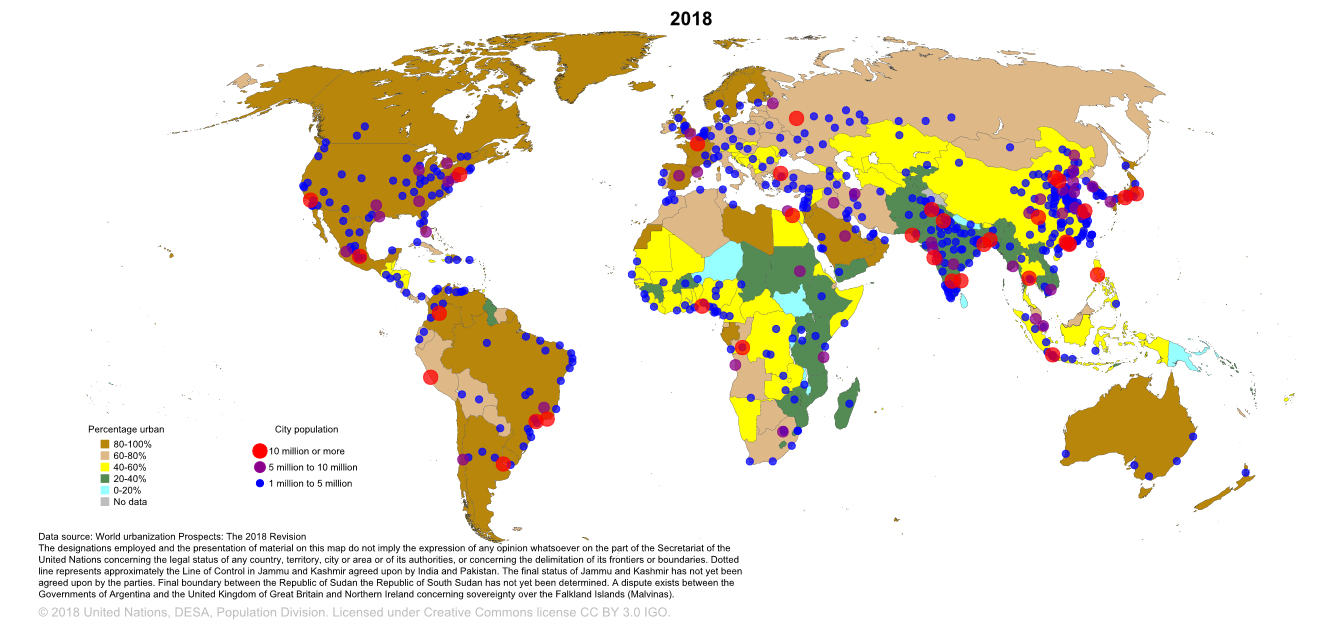
\includegraphics[width=20cm]{image_folder/CityPop_Urban.png}
\caption{Urbanisierung der Welt}
\label{figUrban}
\end{figure}

\FloatBarrier
In der obigen Abbildung erkennt man, dass Nord- und Südamerika sowie Europa deutlich verstädtert sind, wohingegen viele Regionen in Afrika und Asien mehr ländliche Gebiete beinhalten. In dieser Forschungsarbeit wird der Stadtbegriff im Bezug zu ihrer fähigen Lebensmittelversorgung und Nachhaltigkeit betrachtet. Daher eignet es sich Städte im Unterschied zu ländlichen Gemeinden zu beschreiben: 

\begin{displayquote} 
„The hallmarks of cities are: (a) a large population that (b) aggregates in a central location with (c) buildings and monuments that (d) represent institutions that organize and facilitate productivity.“ \footcite[S.16]{Elmqvist2013}. 
\end{displayquote}  Zusammenfassend heißt es, dass Städte sich kennzeichnen lassen durch eine große Einwohnerzahl angehäuft an einem zentralen Ort mit Bauten und Monumenten, die Institutionen repräsentieren und produktive Leistungen organisieren und ermöglichen.

\subsubsection{Stadtökosysteme}
Stadtökosysteme sind Ökosysteme, die von Menschen erzeugt und beeinflusst werden. Wesentliche Merkmale eines Stadtökosystems sind der hohe Anteil an bebauter und versiegelter Fläche und eine hohe Bevölkerungsdichte. Genauer gesagt führt diese hohe Dichte an verschiedenen Landnutzungen dazu, dass natürliche Ressourcen wie Wasser, Luft, Boden und Biodiversität extrem beansprucht werden. Desweiteren lässt sich über Stadtökosysteme sagen, dass ihr Erhalt von der externen Einfuhr an Lebensmitteln und Ressourcen abhängig ist.  \footcite[S.61]{Breuste2016Stadtokosysteme}


\subsection{Urbane Landwirtschaft}

\subsubsection{Urban***}
\begin{flushright}
\textit{MS}
\end{flushright}
Um den Begriff urban oder Urbanität innerhalb der folgenden Forschungsarbeit zu definieren, wird zum Teil die allgemeine Definition „städtisch“ als auch „für eine Stadt charakteristisch“ verwendet.\footnote{Duden, allgemeingültige Definition, urban} Darüber hinaus werden soziokulturelle Aspekte wie die Verwendung des Begriffes im Zusammenhang mit politischen Sichtweisen wie z.B. Weltoffenheit nicht tiefer in die Definition einfließen. Innerhalb der Forschungsarbeit wird der Begriff des Urbanen oder die Urbanität primär mit der physischen Stadt oder „innerhalb einer Stadt“ und verwendet. Randgebiete einer Stadt oder werden hier nicht als urban beschrieben sondern als "Peri-Urban" (siehe Bild).\footcite[S. 140]{MullerUrbanStadt}

\begin{figure}[htbp]
\centering
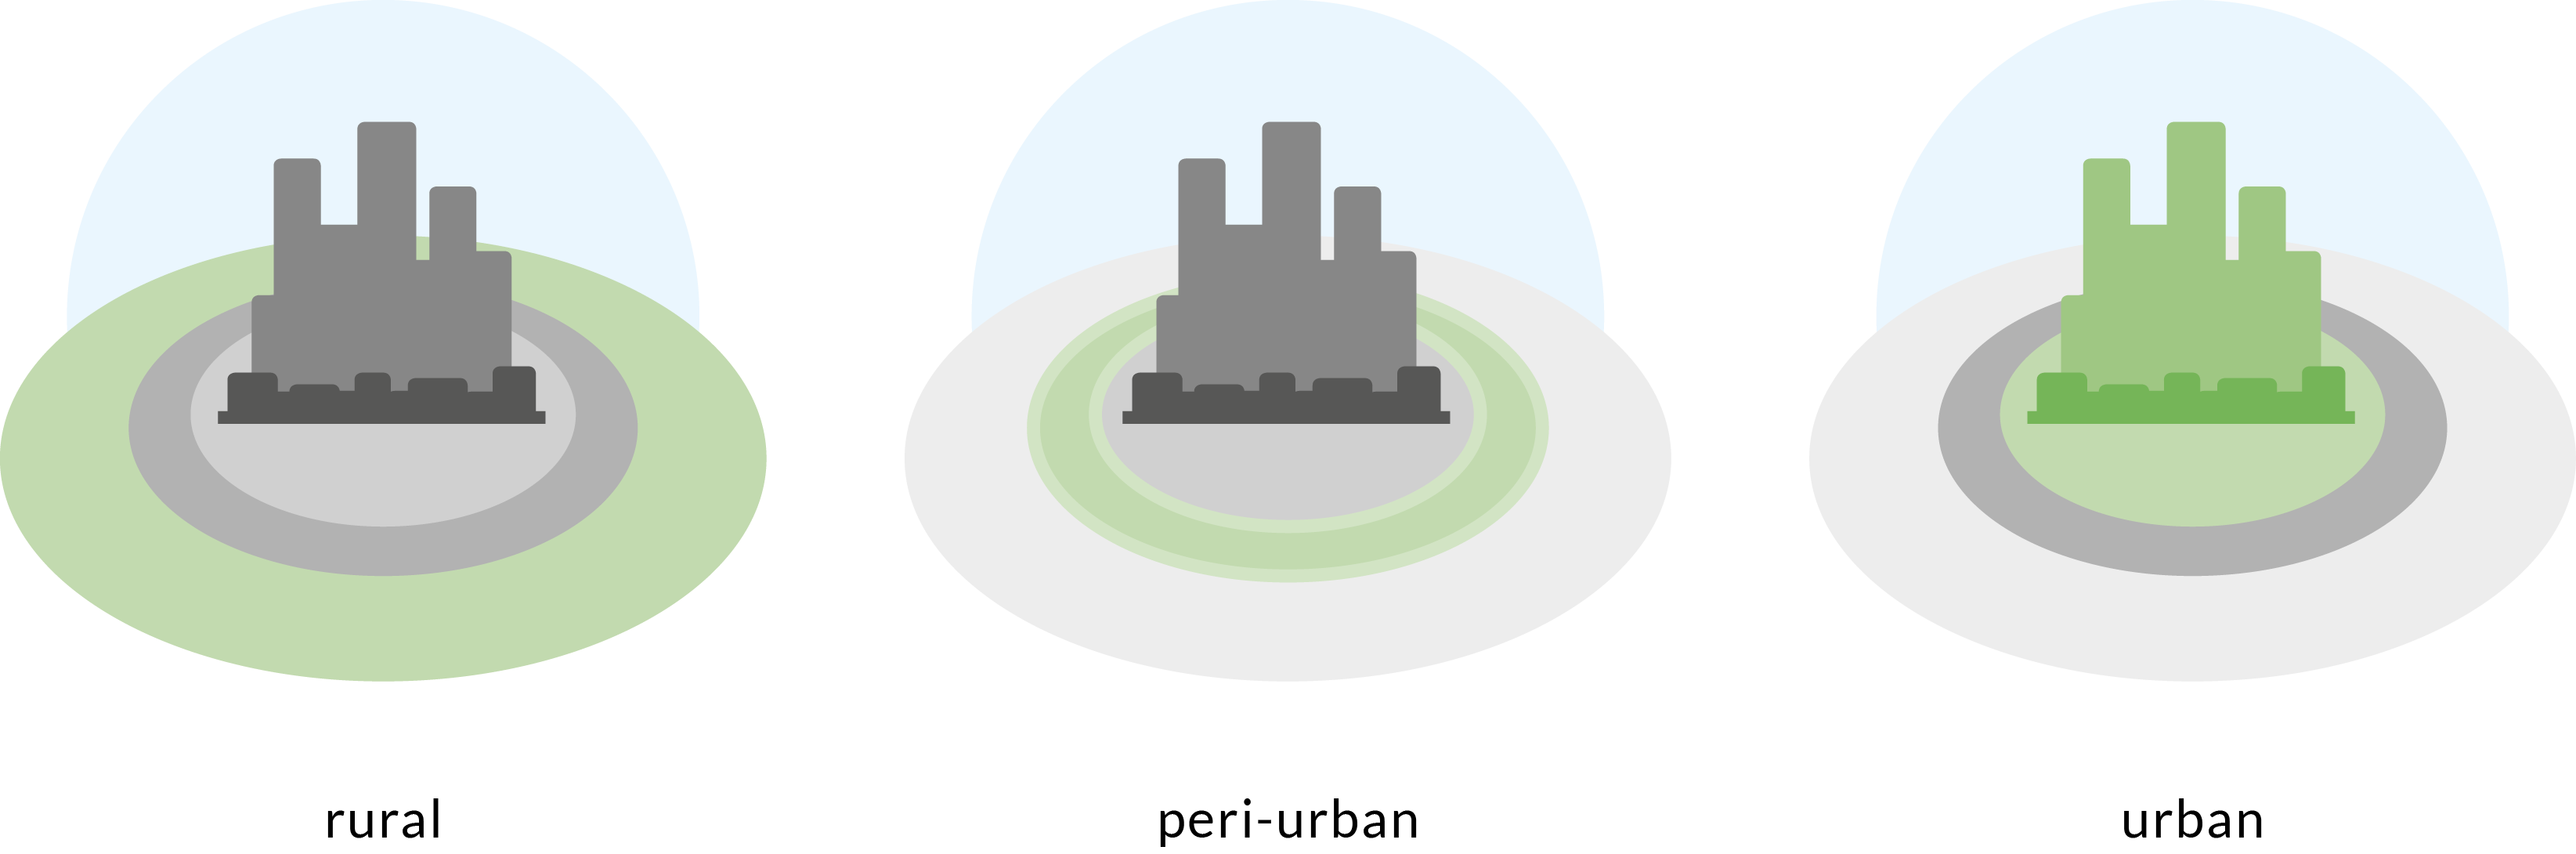
\includegraphics[width=12cm]{image_folder/SchaubildUrbaneEingrenzungen.png}
\caption{Skizze zur räumlichen Einordnung}
\end{figure}
\footcite[]{Eigene Zeichnung, entstanden aus dem Vorbild von Carlos Tobisch, Oasen im Beton S.26, Abb.7}

\subsubsection{Landwirtschaft***}\textit{MS}
Als Landwirtschaft wird der planmäßige Anbau von Nutzpflanzen oder die Zucht und Haltung von Tieren zur Lebensmittel- oder Rohstoffproduktion beschrieben. Die Landwirtschaft umfasst dabei den Nutzpflanzenanbau, die Tierhaltung, den Ackerbau, die Aquakultur und die Imkerei sowie die Fischerei. \footcite[S. 5]{Lohrberg2001StadtnaheFreiraumplanung}  Laut Definition des BauGB § 201. wird unter Landwirtschaft „insbesondere der Ackerbau, die Wiesen- und Weidewirtschaft, einschließlich Pensionstierhaltung auf überwiegend eigener Futtergrundlage, die gartenbauliche Erzeugung, der Erwerbsobstbau, der Weinbau, die berufsmäßige Imkerei und die berufsmäßige Binnenfischerei“ verstanden.\footcite[§ 201]{}

\subsubsection[UL]{Urbane Landwirtschaft***}\textit{MS}
Urbane Landwirtschaft (im folgenden UL genannt) umfasst professionelle landwirtschaftliche und gartenbauliche Aktivitäten in und am Rande von städtischen Siedlungsräumen. Dabei kann die urbane Landwirtschaft durchaus auch weltmarktorientiert sein und lässt sich nach Regine Berges in verschiedene Typen einordnen.\footcite[]{} Die unterschiedlichen Typen von urbaner Landwirtschaft können anhand von verschiedenen Kategorien eingeordnet werden. Die Akteure zum Beispiel bilden die Haupthandelnden einer gärtnerischen Aktivität ab. Dies können Privathaushalte, Kleingruppen, Gemeinschaften oder auch privatwirtschaftlich handelnde Unternehmen sein. 

\begin{itemize}
\item Die Subsistenszausrichtung also die Selbstversorgung hat das Ziel den Nahrungsbedarf durch UL teilweise oder ganz zu decken oder auch um Zugang zu Bio-Lebensmitteln zu erhalten. Diese Ausrichtung wird oft von Privatpersonen und Privathaushalten betrieben. 
\item Mit der soziokulturellen Ausrichtung, die von Gemeinschaften und Vereinen betrieben wird, wird der soziale Austausch in Gemeinschaften gefördert. 
\item Bei der kommerziellen Ausrichtung wird gezielt Einkommen generiert. Der Wachstum des Unternehmens und des Profits steht im Vordergrund. 
\end{itemize}

Parallel dazu kann festgestellt werden für wen, also auf welchen Ebenen, die Nahrungsmittel angebaut und vertrieben werden:

\begin{itemize}
\item Auf der Mikroebene steht die Verteilung der Erzeugnisse an die Familie im Vordergrund.
\item Auf der Mesoebene werden die Erzeugnisse mit einem geschlossenen Kreis an Menschen geteilt wie zum Beispiel Vereinsmitglieder oder Bekannte.
\item Auf der Makroebene werden die Erzeugnisse nicht mehr innerhalb von bestimmten Gruppen geteilt sondern gelangen an Konsumenten, die in der Regel keinem bestimmten Kreis angehören. 
\end{itemize}

Im Fokus dieser Arbeit steht UL auf der Meso- bis Makroebene. Auf diesen Ebenen lassen sich Formen der UL auf deren Ökonomie und Nachhaltigkeit untersuchen.

\begin{figure}[htbp]
\centering
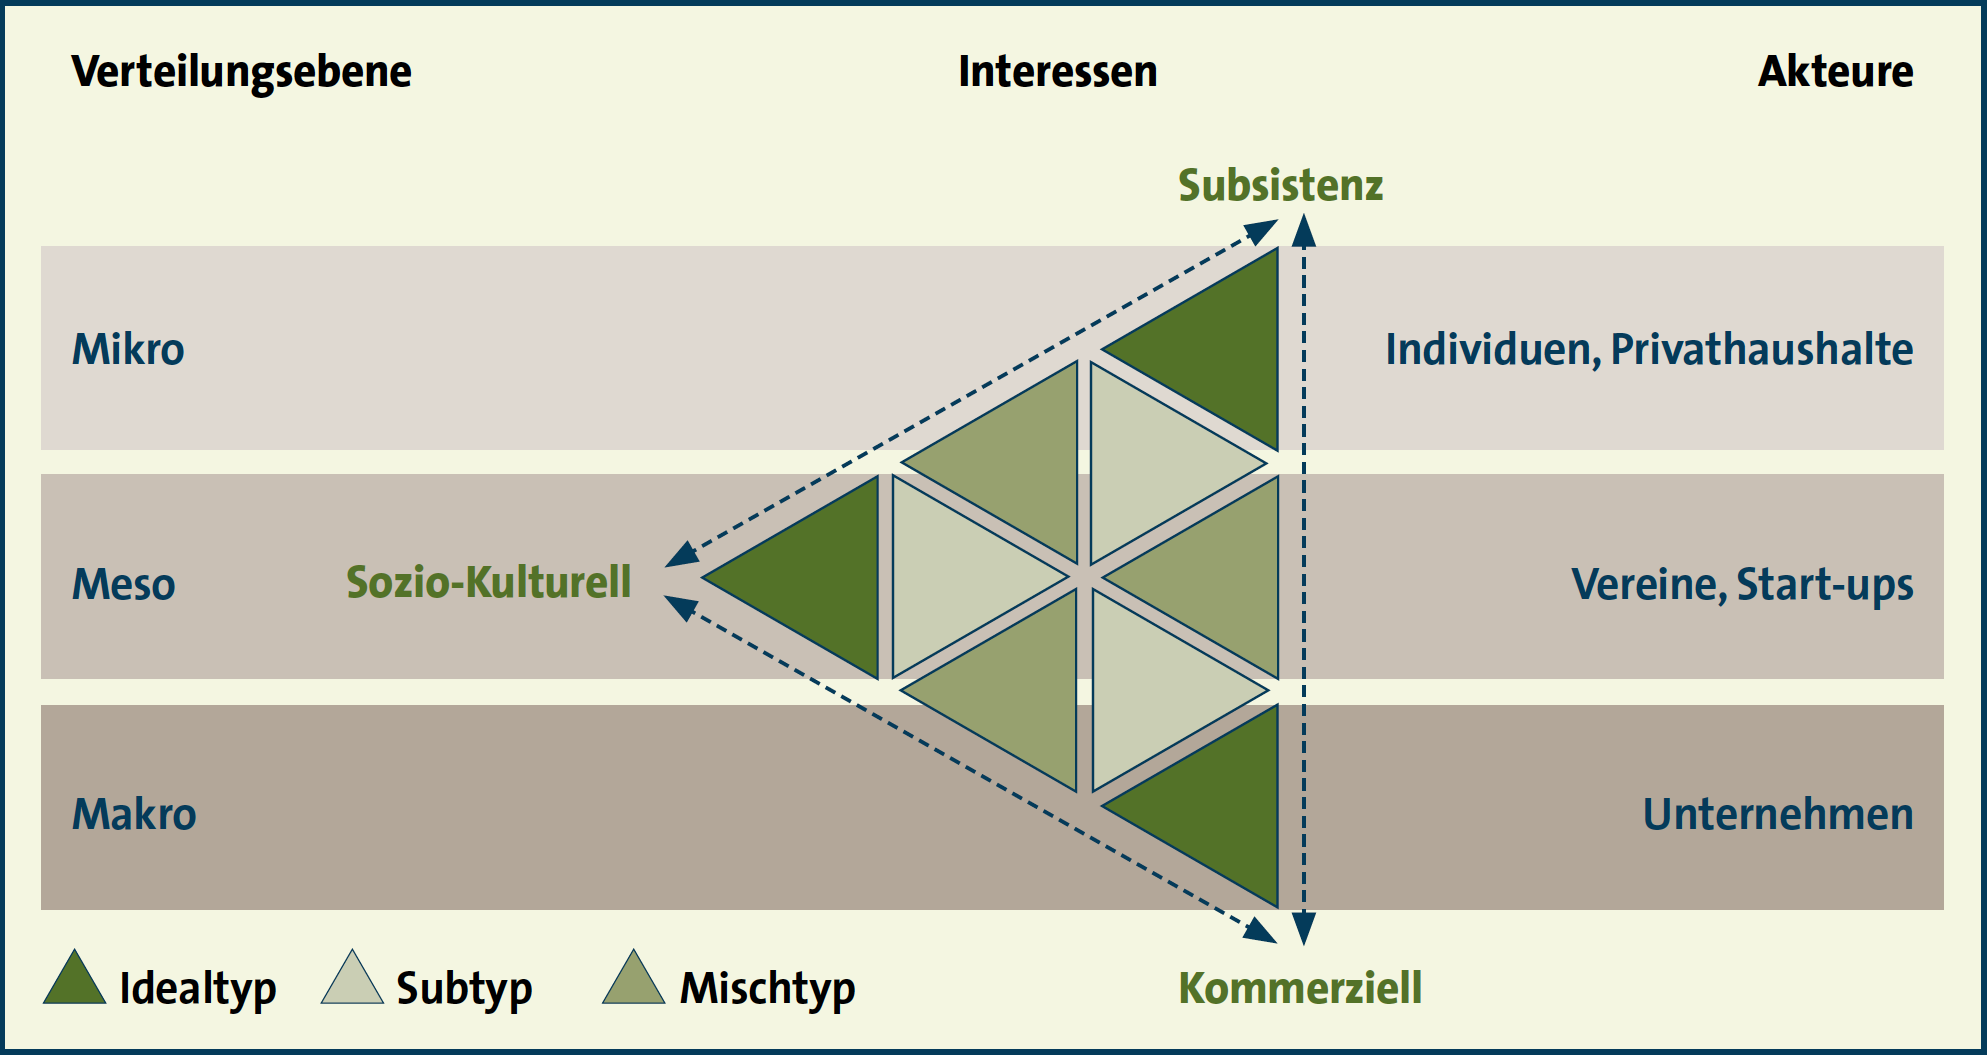
\includegraphics[width=12cm]{image_folder/ul_typologie.png}
\caption{Darstellung der Typologie urbaner Landwirtschaft nach Berges et. al}
\label{fig:ul_typologie}
\end{figure}

\subsubsection{Urban Gardening***}\textit{MS}

Angefangen als Trend in wenigen Metropolen hält Urban Gardening (UG) auch Einzug in immer mehr kleine und mittelgroße Städte. Auch die Kommunalpolitik greift mittlerweile auf das Konzept zurück. Zusammengefasst ist UG die gärtnerische Nutzung städtischer Flächen. Dabei wird UG nicht nur von engagierten Städtern praktiziert sondern auch von professionellen Landschaftsgestaltern und Mitarbeitern der Stadt. Das urbane Gärtnern wird dabei häufig benutzt um ungenutzte Flächen zu begrünen, Klimapolitik zu betreiben, städtische Räume qualitativ aufzuwerten oder Hobbygärtnern eine Fläche zu bieten. UG ist ein Konzept, welches mit aktuellen gesellschaftlichen, politischen und städtischen Entwicklungen eng zusammenhängt.
UG stellt hierbei einen Teil der Urbanen Landwirtschaft dar. Und wird häufig auf der Mikro- bis Mesoebene praktiziert. Einen Unterschied zur Makroebene weist UG insofern auf, dass es sich hierbei um eine oft stark politisch und sozial ambitionierte Bewegung handelt oder die Subsistenz im Vordergrund steht. Die UG-Bewegung hat ihren Fokus verstärkt auf soziale und ideelle Aspekte. Die Makroebene der Urbanen Landwirtschaft zeichnet sich im Gegenzug dazu durch einen professionellen Umgang mit dem Anbau von Lebensmitteln aus. Hier steht die Produktion für den Verbrauchermarkt im Vordergrund. \footcite[S.27]{}

\begin{figure}[htbp]
\centering
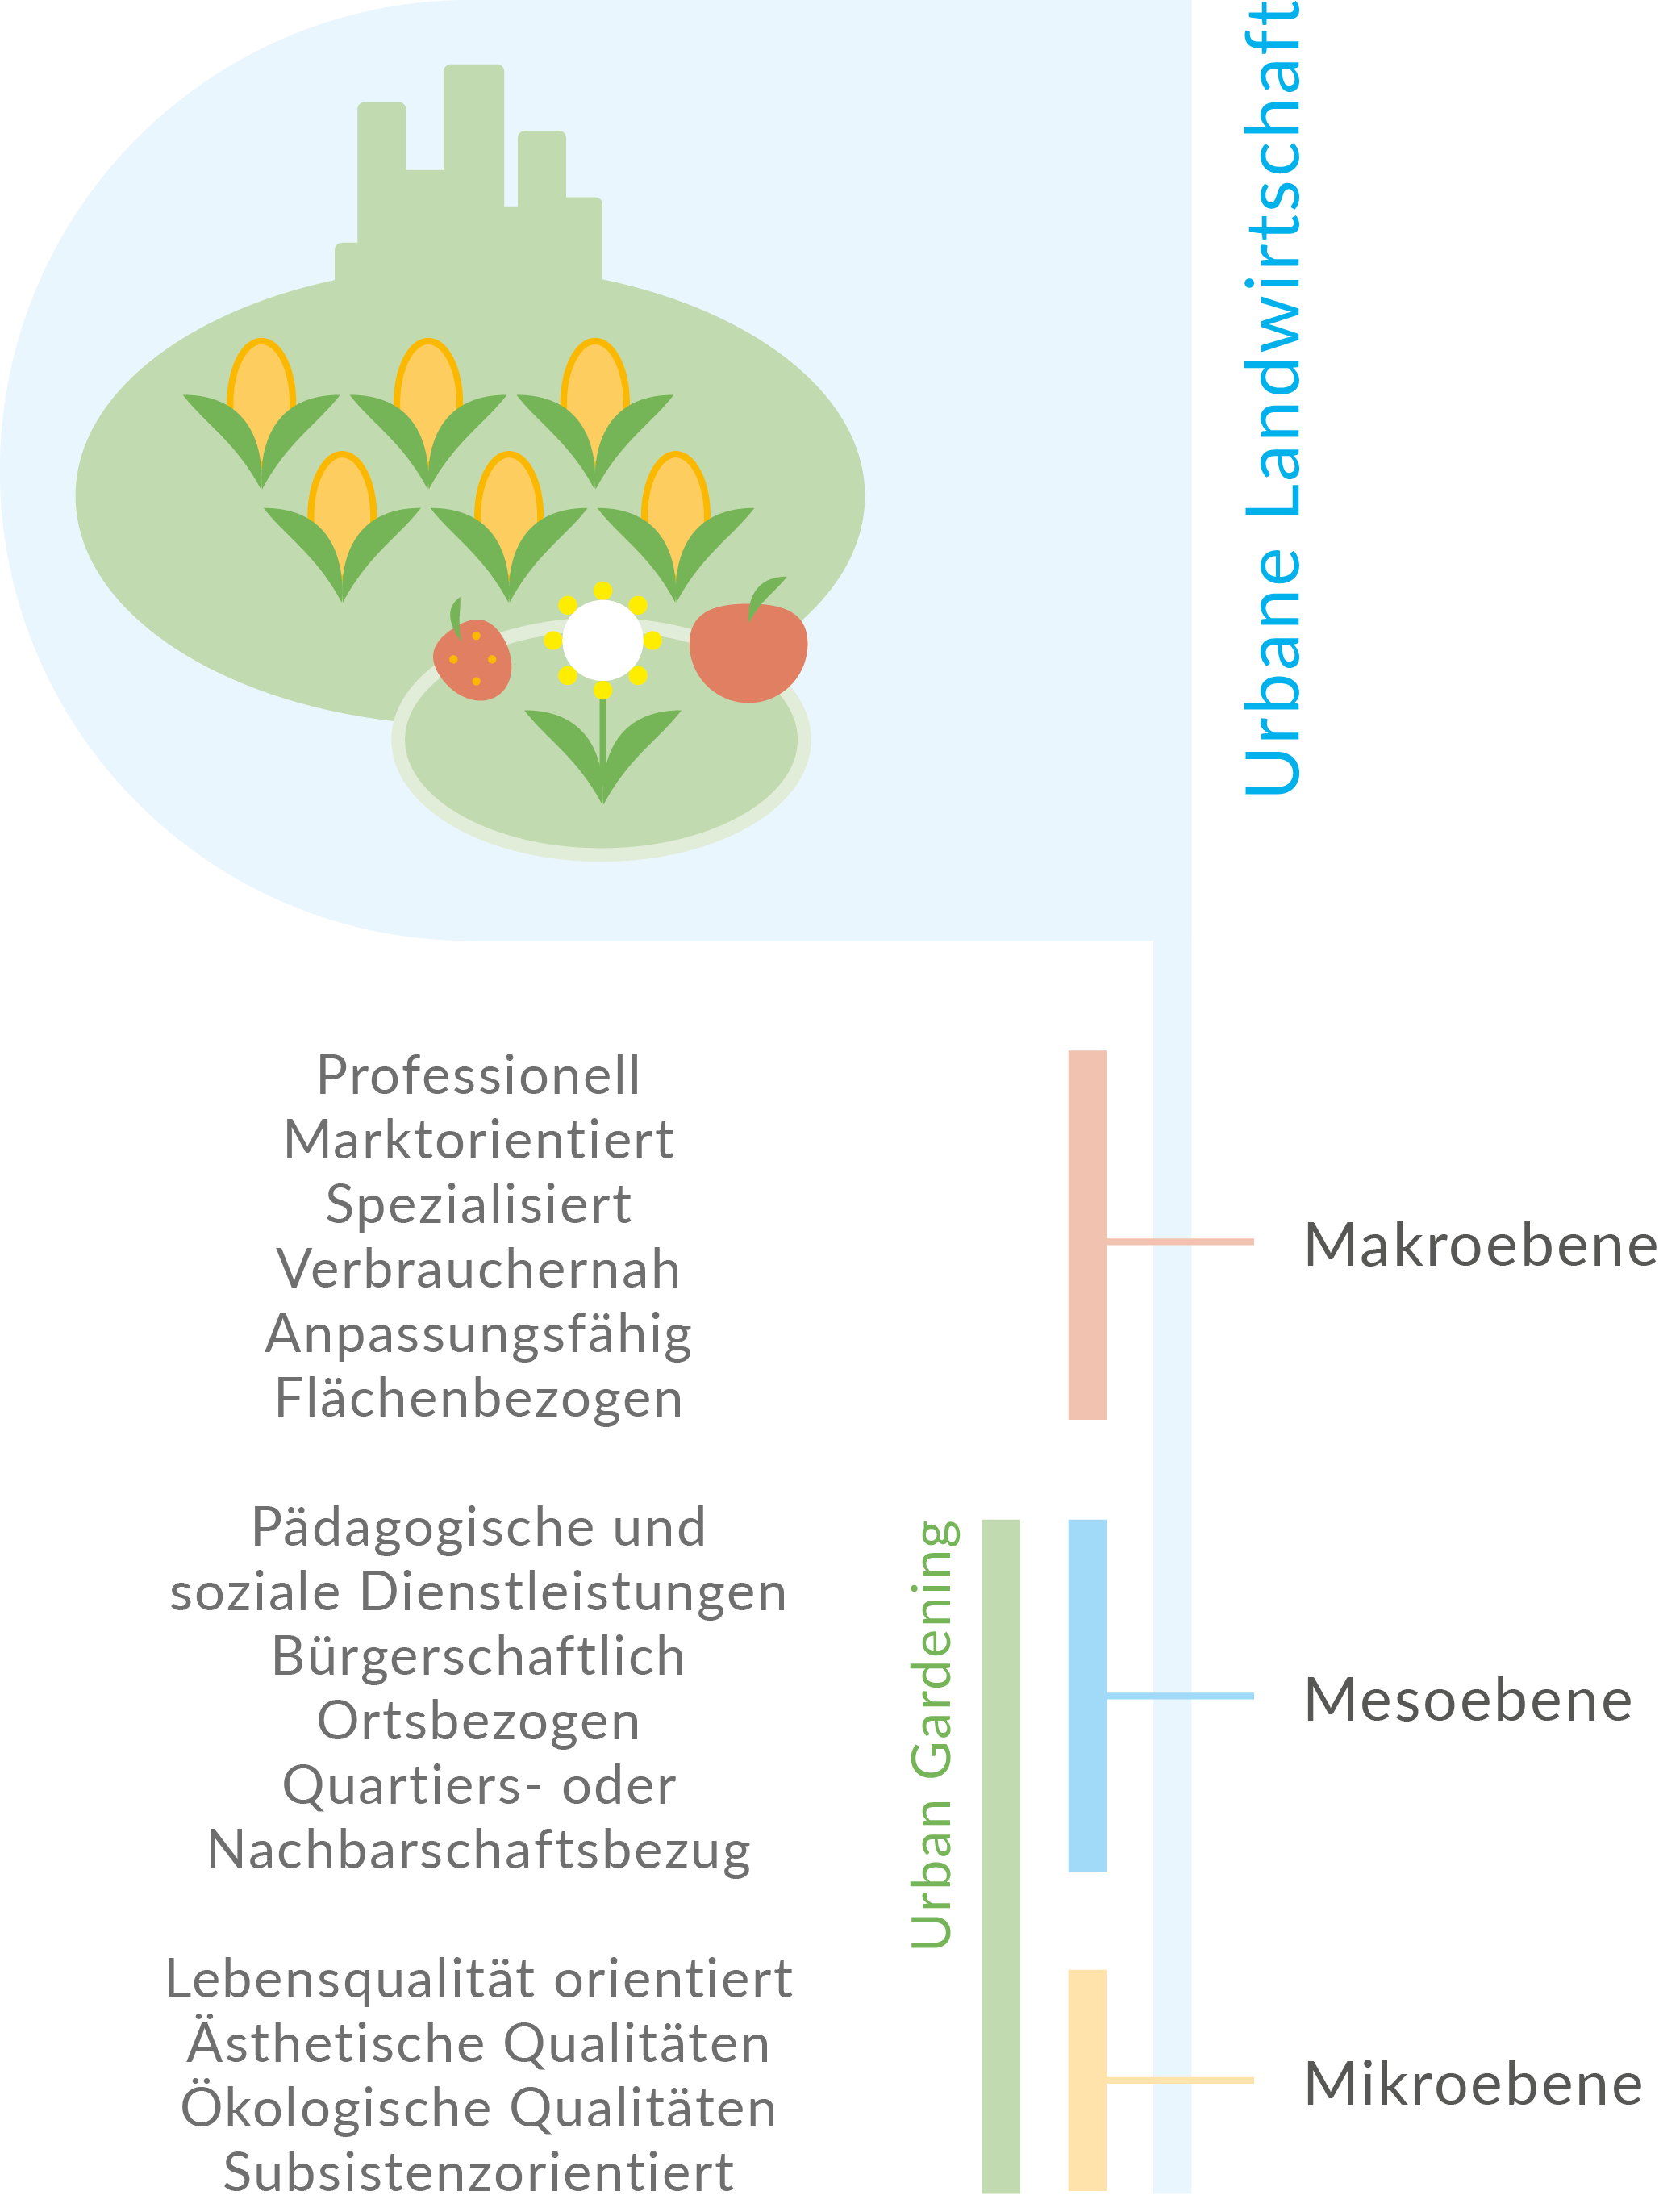
\includegraphics[width=12cm]{image_folder/SchaubildULvsUG.png}
\caption{Eigene Zeichnung, entstanden aus dem Vorbild von Carlos Tobisch, Oasen im Beton (S.27, Abb. 1)}
\label{fig:ul_typologie}
\end{figure}

\subsection{Lebensmittelversorgung}

Aufgrund der steigenden Anzahl der Weltbevölkerung und der sich verändernden globalen Essgewohnheiten entsteht ein steigender Bedarf an Anbaufläche um diesen Lebensmittelbedarf zu decken. Vor allem in Entwicklungsländern und deren städtischen Regionen werden mehr tierische Produkte (d.h. Fleisch- und Milchprodukte), Zucker, Pflanzenöle und verarbeitete Lebensmittel konsumiert als in früheren Jahren. \\
\\Getreide habe laut Von Koerber einen Anteil von 50\% des Nahrungsmittelkonsums weltweit. Das lasse sich vor allem darauf zurückführen, dass in Entwicklungsländern dieser Anteil bis zu 80\% ausmache.\footcite[Vgl.][S.4ff]{VonKoerber2008Globale-trends}
Betrachte man diesbezüglich die Entwicklung aller „Verwendungen (einschließlich Nahrung, Futtermittel und andere Verwendungen, wie Saatgut oder Produktion von Ethanol und Stärke), soll[e] der weltweite Verbrauch von Getreide ansteigen, von 309 kg pro Person im Jahr 2000 auf zu erwartende 339 kg bis 2050.\footcite[S.3ff]{VonKoerber2008Globale-trends}\footcite[vgl.][S.23ff]{FAO2006World2030/2050} 
Laut Keyzer et al. zufolge würden die Prognosen „die Nachfrage nach Getreide als Futtermittel oft stark unterschätzen.
Demnach könnte die Futtergetreidenachfrage in den kommenden Jahrzehnten höher sein, als bis jetzt prognostiziert.”\footcite[S.3f]{VonKoerber2008Globale-trends}

Andere Quellen relativieren diese Aussage und sprechen von einer früheren Sättigung als erwartet.

Ebenso soll der weltweite Konsum von Fleisch, Milch, Milchprodukten und Eiern laut Prognosen weiter steigen. \footcite[Vgl.][S.4f]{VonKoerber2008Globale-trends} So soll sich der Fleischkonsum bis zum Jahr 2050 weltweit verdoppeln und der Milchkonsum um ein Viertel ansteigen. Hierbei bestehen jedoch große regionale Unterschiede.\footcite[Vgl.][S.4]{VonKoerber2008Globale-trends} Während sich der Verbrauch in den Industrieländern bereits einer Sätttigung annähert, steigt der Konsum in Schwellen und Entwicklungsländern noch lange. Der Grund dafür ist dort der Anstieg der Lebensqualität und ein daraus folgender steigender Konsum von Luxusprodukten.

\begin{figure}[htbp]
\centering
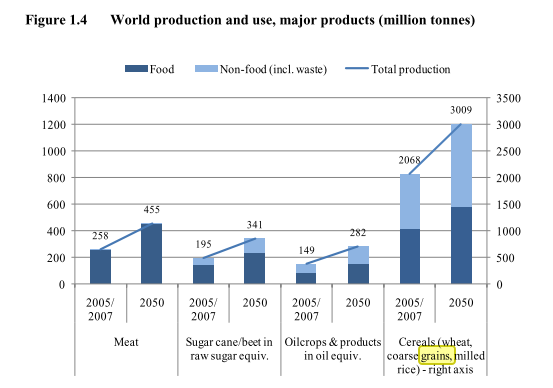
\includegraphics[width=16cm]{image_folder/2030S8.png}
\caption{Weltweiter Anstieg des Lebensmittelkonsums bis 2050}
\label{fig:konsumbis2050}\footcite[vgl.][S.8]{FAO2006World2030/2050} 
\end{figure}

\begin{figure}[htbp]
\centering
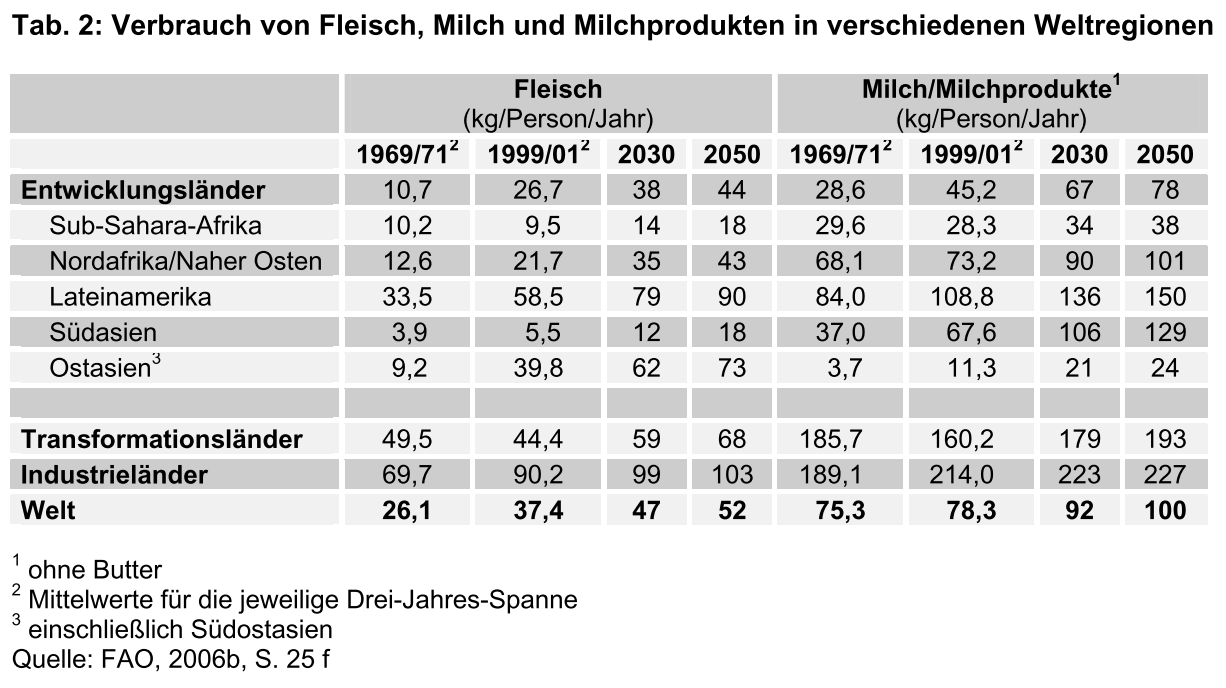
\includegraphics[width=16cm]{image_folder/KonsumWeltweit.png}
\caption{Weltweiter Konsum von Lebensmitteln}
\label{fig:konsumweltweit}\footcite[S.4f]{VonKoerber2008Globale-trends}
\end{figure}


\subsubsection{Flächenbedarf von Ernährungsgewohnheiten}

Etwa 38 \% der weltweit vorhandenen Landfläche (d.h. ungefähr 5Mrd ha) stehen für landwirtschaftliche Nutzung zur Verfügung. Der größte Teil mit 69\% hiervon ist Weideland (mit ungefähr 3,4 Mrd. ha). 28\% der landwirtschaftlichen Nutzfläche ist Ackerland und nur 3\% Dauerkulturen.
Da etwa ein Drittel des Ackerlands der Futtermittelproduktion dient entsteht so der Wert von 80\% der gesamten landwirtschaftlichen Nutzfläche der für die Tierhaltung gebraucht wird. Aus diesen 80\% der landwirtschaftlichen Fläche wird allerdings nur ein Anteil von 17\% (3,4 Mrd. ha) der weltweiten Nahrungsmittelversorgung gedeckt. \footcite{2008FAOSTAT}\footcite[Vgl.][S.6]{VonKoerber2008Globale-trends}


\begin{figure}[htbp]
\centering
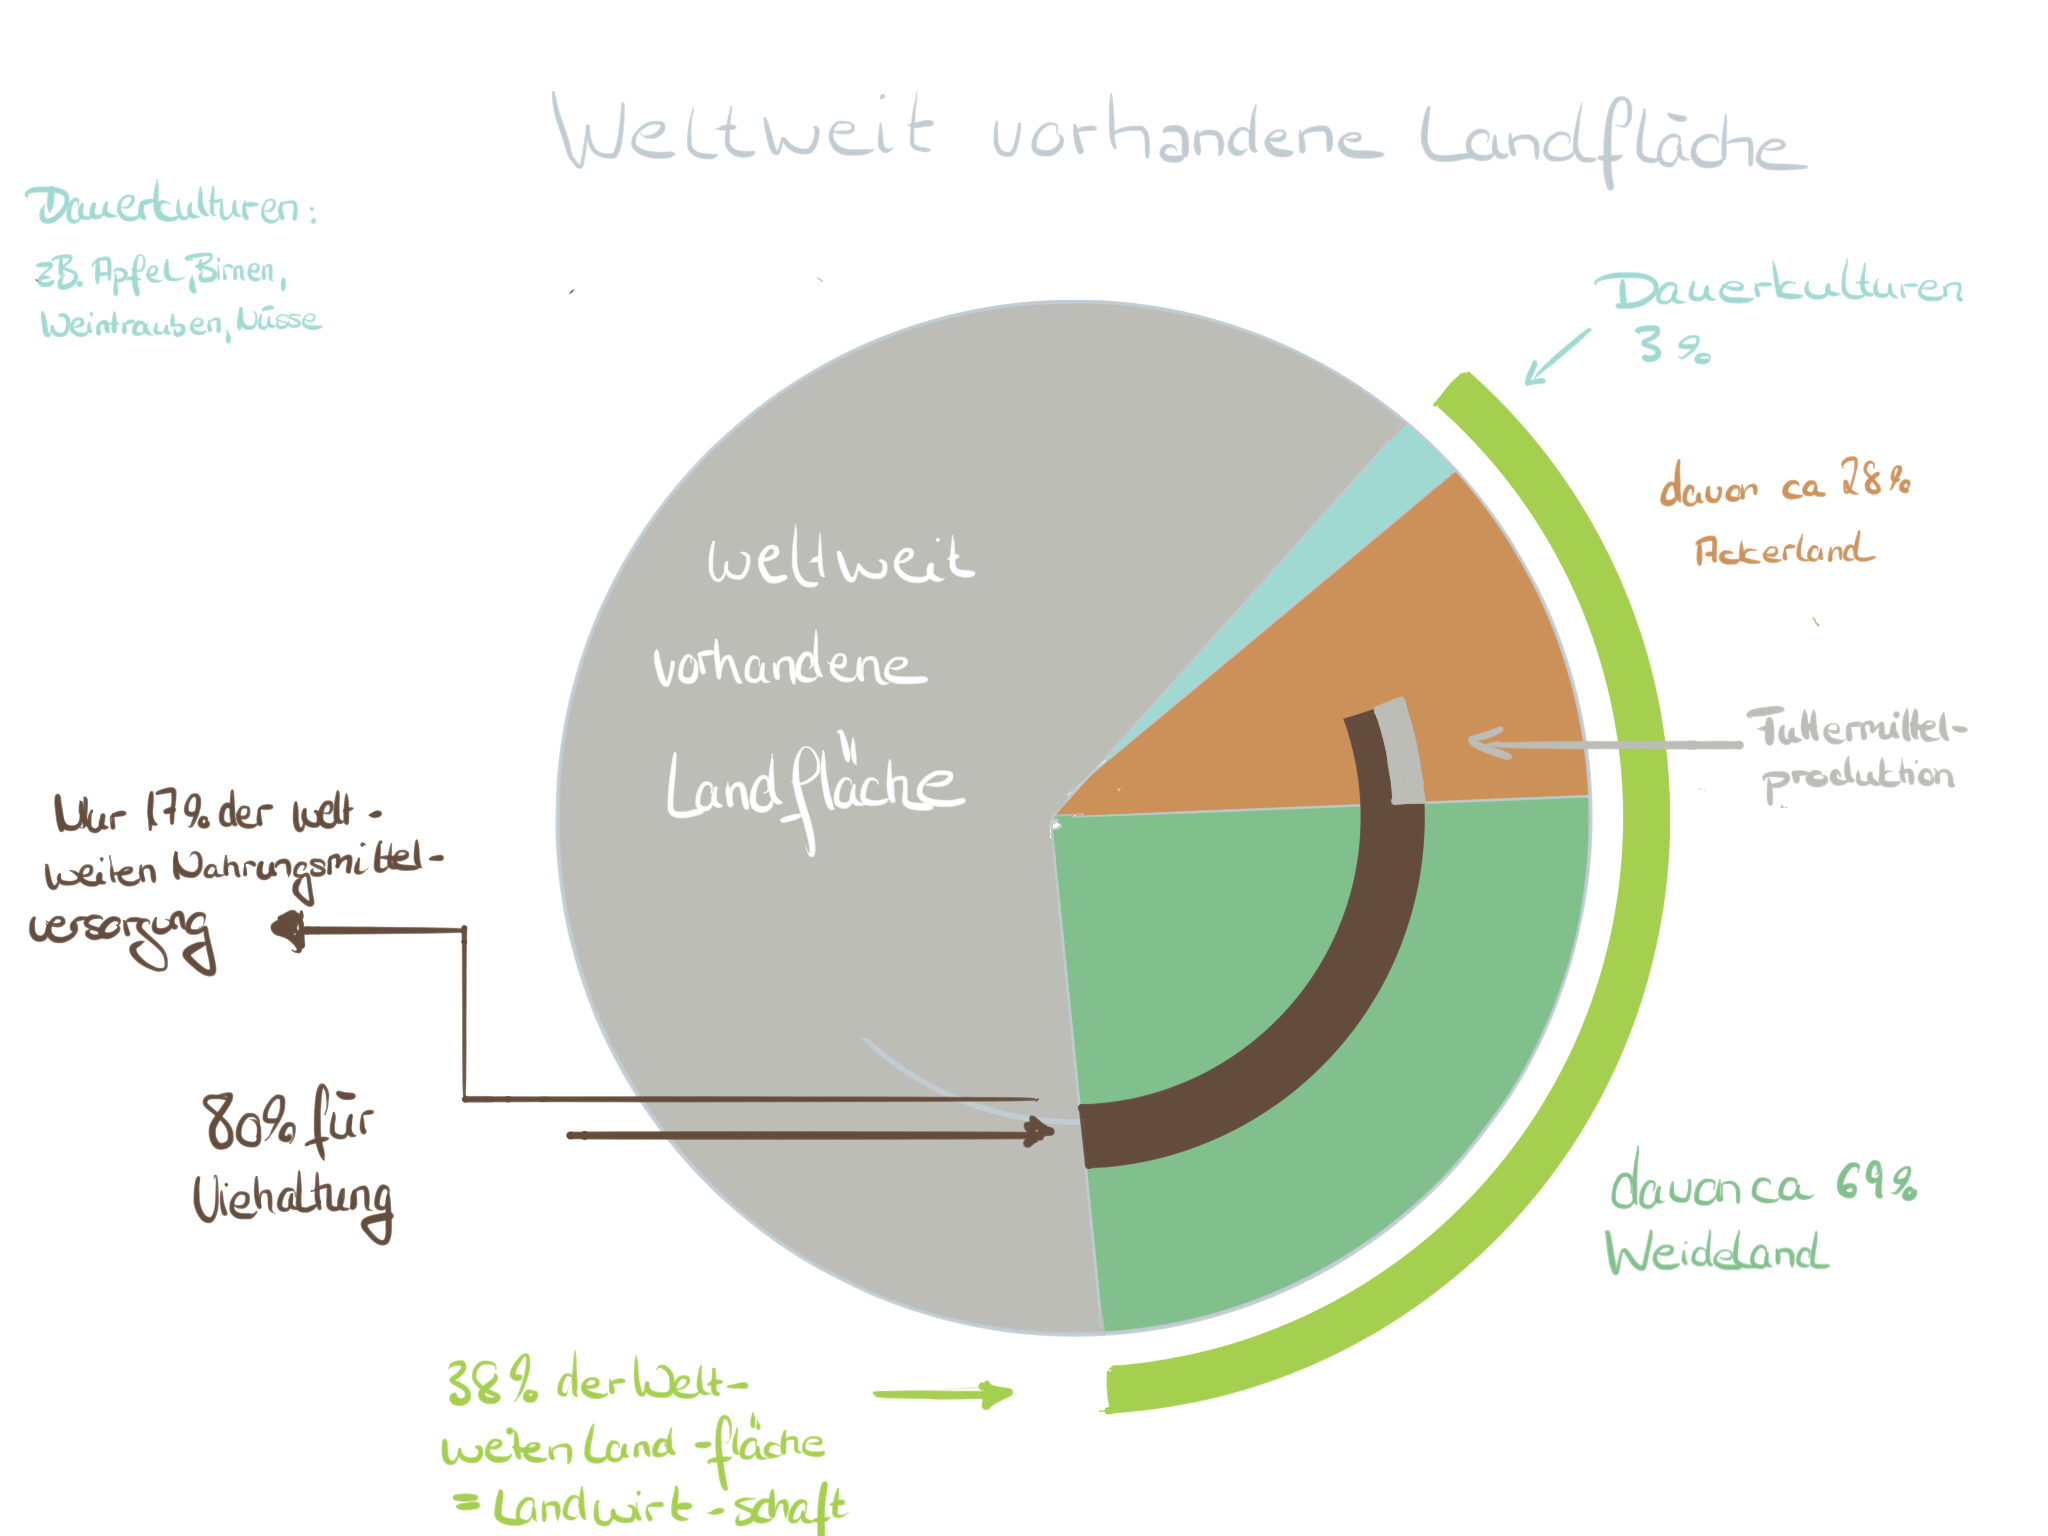
\includegraphics[width=10cm]{image_folder/LFlaeche.png}
\caption{Weltweite Nutzung von landwirtschaftlicher Fläche}
\label{fig:lFlaeche}
\end{figure}\footcite[Eigene Darstellung in Anlehnung an]{2008FAOSTAT}

Wie in \label{fig:AckerproKopf} zu beobachten ist, wird mit dem weiteren Wachstum der Weltbevölkerung die vorhandene Ackerfläche pro Kopf kleiner. 

\begin{figure}[htbp]
\centering
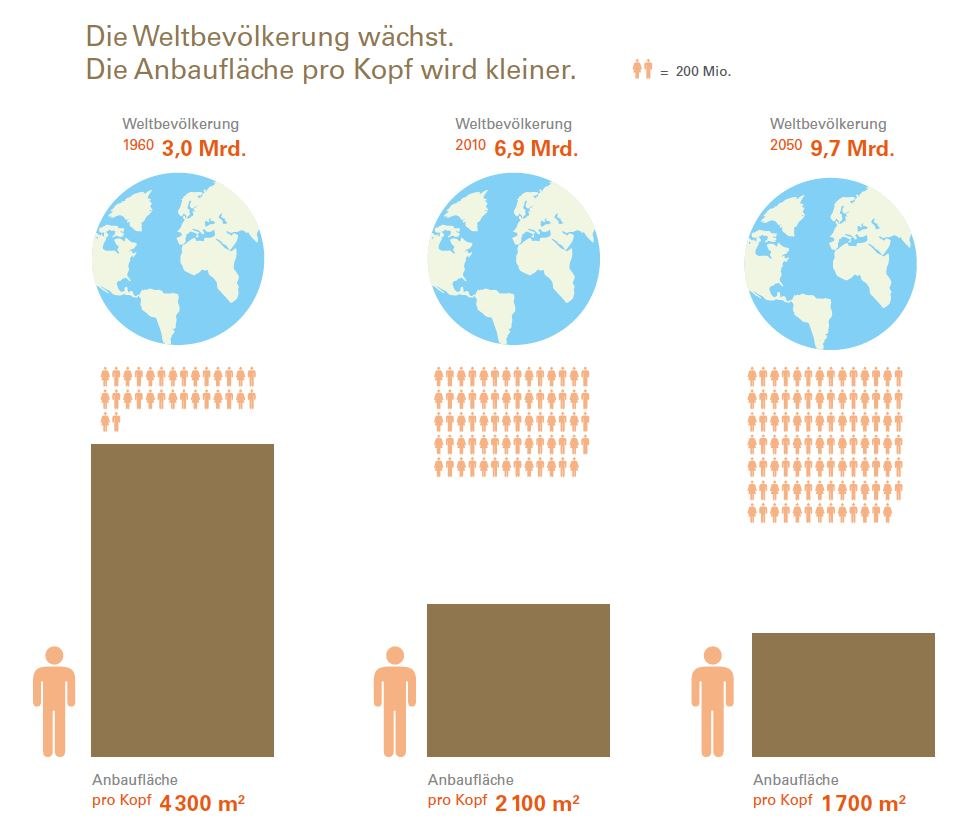
\includegraphics[width=10cm]{image_folder/weltbevoelkerung_anbauflaeche_pro_kopf.jpg}
\caption{Weltweite vorhandene Ackerfläche pro Kopf}
\label{fig:AckerproKopf}
\end{figure}

\subsection{Nachhaltigkeit***}

Der Begriff Nachhaltigkeit an sich ist ein vielschichtiger Begriff. Er findet Verwendung in der Wirtschaft, Ökonomie, Ethik und Ökologie. Nachhaltigkeit kann als Art und Weise des Wirtschaftens bezeichnet werden, „bei welcher derzeitige Bedürfnisse befriedigt werden, ohne zukünftigen Generationen die Lebensgrundlagen zu entziehen. \footcite{DefinitionWirtschaftslexikonb}. Ebenso kann der Begriff als Brücke zwischen ökologischen und ökonomischen Interessen verstanden werden. Seinen Ursprung hat das Prinzip der Nachhaltigkeit in der Forstwirtschaft des 18. Jahrhunderts. Nach einer Übernutzung der Wälder und daraus resultierend knapper werdenden Holzbeständen, wurde mit Nachhaltigkeit ein Bewirtschaftungsprinzip gefordert, bei dem regenerativ gearbeitet werden sollte, das heißt “nicht mehr Holz geschlagen werden als nachwächst.“ \footcite{NachhaltigeBrockhaus.de}
Ab dem 19. Jahrhundert wurde dieser rein ressourcenökonomischen Betrachtungsweise von Nachhaltigkeit eine umfassendere hinzugefügt, die sämtliche Funktionen des Waldes in Betracht zieht, wie beispielsweise die Aufrechterhaltung seiner Schutzfunktion.\footnote{was versteht man unter nachhaltigkeit!!!!!!!!!!!!!!!!1}

\hfill \break
Der Begriff Nachhaltigkeit kann in „stark” und „schwach” eingeteilt werden.\footcite{Nachhaltigkeit}


\begin{itemize}
\item die starke Nachhaltigkeit stellt die Erhaltung der natürlichen Ressourcen in den Vordergrund. Sie beruht auf der Annahme, dass Naturgut nicht durch andere Kapitalformen ersetzt werden kann.
\item schwache Nachhaltigkeit beruht auf der Annahme das Kapital- oder Naturgut durch andere Kapitalformen ersetzt werden kann.
\end{itemize}
Konfliktpotenzial zwischen den Vertretern jeweiliger Positionen tritt vor allem bei der Frage auf, „wie heute verursachte, aber zukünftig auftretende Umweltschäden beziehungsweise Ressourcenknappheiten zu bewerten sind".\footcite{NachhaltigeBrockhaus.de}



\subsubsection{Nachhaltige Entwicklung}
  Ziel der nachhaltigen Entwicklung ist eine dauerhalfte und gerechte Bewirtschaftung der Erde.\footcite{NachhaltigeBrockhaus.de} Die Bezeichnung wurde vom Begriff der Nachhaltigkeit abgeleitet. In der Agrar- und Ernährungswirtschaft definiert der Begriff eine "dauerhafte Nutzung von Ressourcen bei gleichbleibender bzw. wachsender Effektivität". \footcite{oppenhauser2010nachhaltigkeit} Im internationalen Sprachraum hat sich der Begriff „Sustainable Development” als Definition gefestigt. In der internationalen Politik und bei gesellschaftlichen Bewegungen wird die nachhaltige Entwicklung als Leitbild eingesetzt.\footcite{oppenhauser2010nachhaltigkeit}
 
 Konkrete Umsetzungsmethoden von nachhaltiger Entwicklung stellen in Entwicklungsländern hauptsächlich Aspekte hinsichtlich des ökonomischen und sozialen Fortschritts in den Vordergrund. In den industrialisierten Ländern geht es dabei mehr um den langfristigen Schutz und Erhalt der natürlichen Lebensgrundlage. 



\subsubsection{Ökologische Nachhaltigkeit***}
„Die ökologische Nachhaltigkeit bezieht sich allgemein auf das Überleben und den Gesundheitszustand von Ökosystemen.“ \footcite{DefinitionWirtschaftslexikonc}  Sie bezeichnet einen weitsichtigeren und rücksichtsvolleren Umgang mit natürlichen Ressourcen. Sofern die ökologische Nachhaltigkeit vernachlässigt wird, kann dies dazu führen, dass bestimmte Ressourcen unbrauchbar oder unwiderruflich zerstört werden, was jegliche weitere Entwicklung der Ressource und ihrer Umgebung unmöglich machen kann. Laut Berding und Bukow in "Die kompakte Stadt der Zukunft - Auf dem Weg zu einer inklusiven und nachhaltigen Stadtgesellschaft (s.95) \footcite{BerdingWolf-DietrichBukowKarinCudakHrsgDieStadtgesellschaft} gewinnt das Thema Nachhaltigkeit für die Stadtentwicklung an neuer Relevanz. 



\subsubsection{Ökosystem***}
Als Ökosystem bezeichnet man ein Wirkungsgefüge von Arten und ihrem Lebensraum. Einzelne Vorgänge innerhalb des Systems werden von Produzenten und Destruenten durchgeführt. Vereinfacht dargestellt entsteht auf diese Weise eine Nahrungskette. Dieses Nebeneinander aus verschiedenen Organismen befindet sich stets in einem zyklischen Prozess. Je enger die Nahrungsketten ineinander verwoben sind und je artenreicher das Wirkungsgefüge ist desto komplexer und resilienter ist das Ökosystem.\footcite{NachhaltigeBrockhaus.de} Die Agrarlandschaft kann als ein vom Menschen stark beeinflusstes und künstliches Ökosystem angesehen werden.\footcite[Vgl.]{BrockhausOkosystem}
Ökosysteme sind offene Systeme, die einseitig von der Sonne Energie aufnehmen. Die Stoffkreisläufe innerhalb des Systems sind unter optimalen Umständen ausgeglichen. So entsteht ein dynamisches Gleichgewicht. \footcite{BrockhausOkosystem}

\hfill \break
Stabilität und Gefährdung: Komplexe Ökosysteme sind stabiler als einfache Ökosysteme, gleichzeitig sind diese schwerer oder unmöglich regenerierbar, während einfache Ökosysteme sich und ihr Gleichgewicht einfach wiederherstellen können. Als Beispiel kann der Vergleich zwischen einem einfachem Ökosystem (Nadelwald) und einem komplexem Ökosystem (Regenwald) herangezogen werden.
In einem einfachen System kann der Verlust oder die Veränderung einzelner Komponenten (Überdüngung, Wasserknappheit oder Überwässerung in Brachregionen) das eigene Gleichgewicht sowie das Gleichgewicht angrenzender Ökosysteme schneller in Gefahr bringen. \footcite{DefinitionWirtschaftslexikone}

\begin{figure}[htbp]
\centering
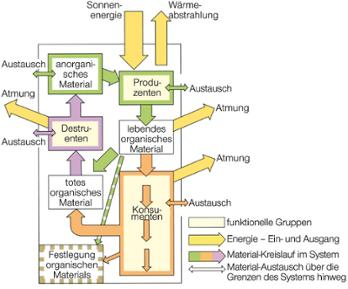
\includegraphics[width=5cm]{image_folder/oekosystemkreisslauf.png}
\caption{Ökosystemkreisslauf: Kreislauf: Verknüpfung von Konsumenten Destruenten und Produzenten}
\label{fig:Ökosystemkreisslauf}
\end{figure}



        
\subsubsection{Öko-Effizienz und Ressourceneffizienz im Vergleich}

Öko-Effizienz und Ressourceneffizienz geben beide eine relative Kennzahl an, die das Verhältnis einer gewünschten Größe zu ihrer unerwünschten (Schadschöpfung) darstellt. Der Fokus ist bei den Begriffen ein anderer. Im Folgenden wird erklärt, inwiefern sich bei den Begriffen die Fokussierung unterscheidet.

\\
\subsubsection{Öko-Effizienz}
Die Öko-Effizienz beschreibt das Verhältnis von ökologischer Schadschöpfung einer Tätigkeit oder eines Produkts zu seiner ökonomischer Wertschöpfung. \footcite[Vgl.][S.]{Schaltegger1990OkologischeUnternehmung} 

\subsubsection{Ressourceneffizienz}
Im Vergleich dazu liegt der Fokus bei der Berechnung der  Ressourceneffizienz beim Ressourcenverbrauch bzw. die Materialflüsse. Die Gleichung wäre hier also: Wertschöpfung/Ressourcenverbrauch.

\begin{figure}[htbp]
\centering
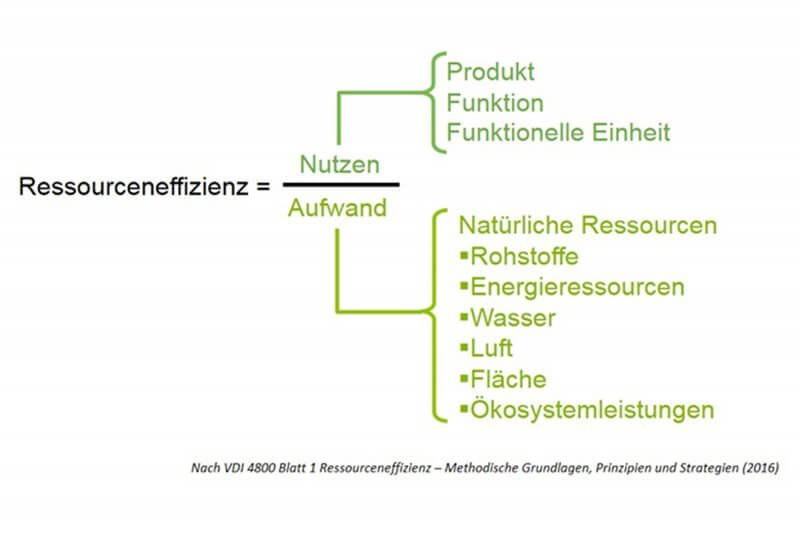
\includegraphics[width=10cm]{image_folder/ressourceneffizienz.jpg}
\caption{Ökoeffizienzgleichung}
\label{fig:Ökoeffizienzgleichung}
\end{figure}\footcite{Essel2010AnalyseFazit}

   
 Der WBCSD\footnote{ein Zusammenschluss international tätiger Unternehmen, der das Ziel hat, Wirtschaftswachstum und Nachhaltigkeit in Einklang zu bringen} hat "für Ökoeffizienz folgende Kriterien erstellt: 
 
 \begin{itemize}
 \item die Bereitstellung wettbewerbsfähiger Produkte
 \item die Befriedigung menschlicher Bedürfnisse 
 \item die Förderung der Lebensqualität
 \item die Minimierung der Umweltauswirkungen und Ressourcenintensität während des gesamten Produktlebens\footcite{OkoeffizienzBrockhaus.de}
 \end{itemize}

Zur nachhaltigen Umsetzung von Produktionsmethoden werden ökoeffiziente Strategien und Konzepte angewendet. Die Kriterien für diese Strategien sind laut WBCSD folgende:
\begin{itemize}
\item geringer Einsatz natürlicher Ressourcen
\item geringe Umweltbelastung
\item zu ersteren beiden im Vergleich hoher Ertrag
\end{itemize}


Ökoeffizienz kann u.a. erreicht werden durch:
\begin{itemize}
\item Minimierung des Material- und Energieverbrauchs pro Produktmenge,
\item Verwendung recyclingfähiger Materialien,
\item Einsatz erneuerbarer Ressourcen, Vermeidung des Einsatzes toxischer Substanzen,
\item Erhöhung der Lebensdauer beziehungsweise des Nutzens eines Produktes.
\end{itemize}\footcite{OkoeffizienzBrockhaus.de}





\subsubsection{Ökosystemdienstleistungen}

\begin{figure}[htbp]
\centering
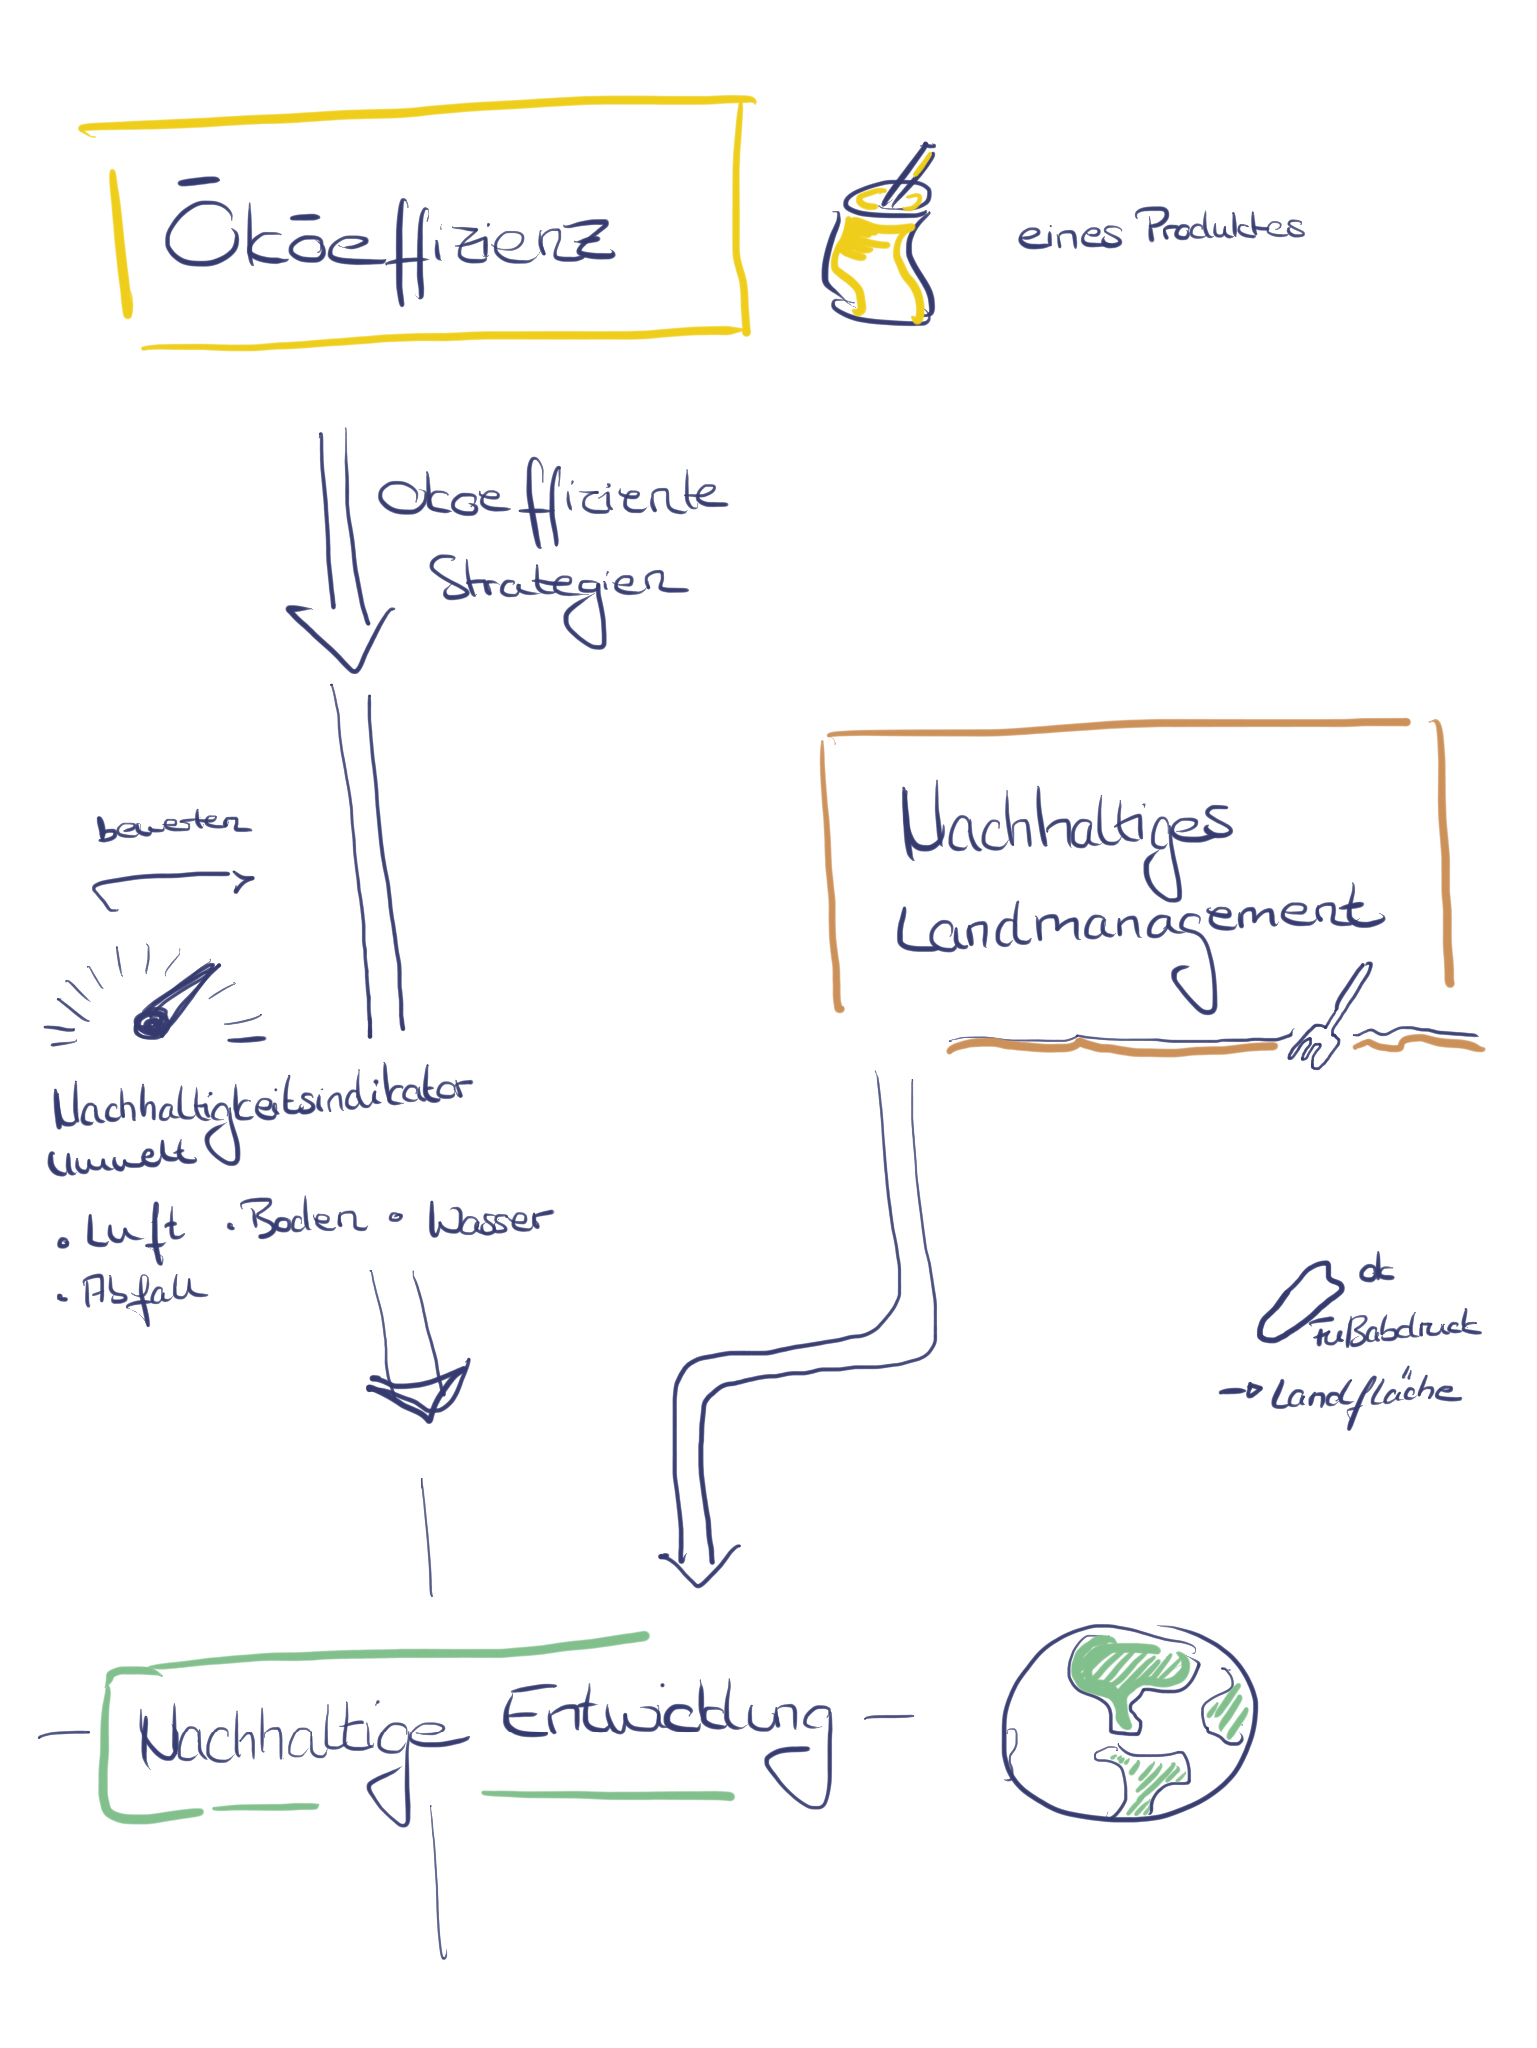
\includegraphics[width=10cm]{image_folder/NE_folgerungen.png}
\caption{Schlussfolgerungen aus Infos zu NE}
\label{fig:Folgerung_NE}
\end{figure}\footcite{Eigene Darstellung}

\subsubsection{Bewertung von Nachhaltigkeit}
Es gibt eine Vielzahl an Werkzeugen zur Bewertung von Nachhaltigkeit. Sie unterscheiden sich je nach Zielsetzung und Fokus. Neben vielen weiteren Methoden hat das Darmstädter Institut IINAS eine Reihe an Methoden als Datenbanken veröffentlicht. Diese sind Folgende:

\begin{itemize}
\item Ökoeffizienz-Analyse der BASF ( diese misst ökologische und ökonomische Dimension) und SEEBALANCE® (ökologische, ökonomische und soziale Dimension)
\item GEMIS - ein „Lebensweg- und Stoffstromanalyse-Modell mit integrierter Datenbank für Energie-, Stoff- und Verkehrssysteme”\footcite{}
\item GLOBALANDS: Entwicklung eines globalen Nachhaltigkeitsstandards zur Landnutzung
\item Nachhaltigkeitsstrategien
\end{itemize}

\subsubsection{Bewertung von Nachhaltiger Landnutzung}
Das Framework for Evaluating Sustainable Land Management FESLM von Smyth \& Dumanski wurde in den 90er Jahren von der FAO (Food and Agriculture Organisation) entwickelt und von Drechsel et al. (2008) erweitert.
\begin{figure}[htbp]
\centering
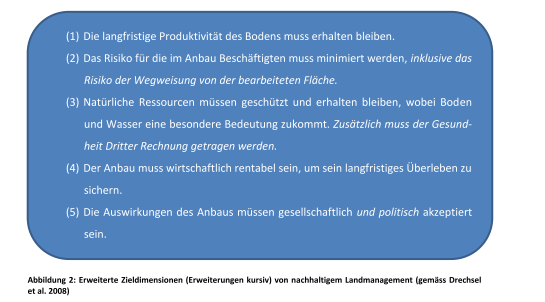
\includegraphics[width=12cm]{image_folder/drechsel.png}
\caption{Bewertung von Nachhaltiger Landnutzung}
\label{fig:Bewertung von Nachhaltiger Landnutzung}
\end{figure}\footcite{Spring2012DerBasel-Stadt, S.17}

\subsubsection{Ökologischer Fußabdruck***}
Weltweit ist der „Ökologischer Fußabdruck einer der erfolgreichsten Indikatoren zur Vermittlung der „physischen Begrenztheit des Planeten Erden”.\footcite[S.2]{StefanGiljum2007WissenschaftlicheFuabdruck}„Die (Natur-)Fläche, die zur Aufrechterhaltung der Energie- und Materialflüsse einer Wirtschaftseinheit wie z. B. einer Stadt benötigt wird, ist deren ökologischer Fußabdruck. Er ist ein Werkzeug zur Bilanzierung des menschlichen Naturverbrauchs und wird in globalen Hektaren angegeben."„Der ökologische Fußabdruck misst so die ökologische Tragfähigkeit’ einer Bevölkerung“.\footcite[S. 25]{MathisWackernagelUnserNimmt} \footcite[S.5]{MichelsenGrundlagenEntwicklung} 
\footcite[Vgl.][S.23ff]{MathisWackernagelUnserNimmt}
„Die Inanspruchnahme von Ressourcen einer Person, einer Stadt oder eines Landes"\footcite[S.192]{AntjeFlade2015StadtStadtforschung} können somit anhand des ökologischen Fußabdrucks verglichen werden. 

\begin{displayquote}
„Der ökologische Fußabdruck von London – als Beispiel für eine Großstadt in einem hoch entwickelten Land – ist z.B. um etwa das Dreihundertfache größer als die Stadtfläche von London (Wackernagel et al. 2006), und damit wird deutlich, dass die Bevölkerung Londons auf ein Vielfaches der Stadtfläche – nicht nur im Umland, sondern weltweit – angewiesen ist. Da die globale Menge an Biokapazität begrenzt ist, veranschaulicht der ÖF ebenso das bestehende Ungleichgewicht.”\footcite{AntjeFlade2015StadtStadtforschung, S.192}
\end{displayquote} 

Durch die Berechnung dieses Fußabdrucks kann also nachvollzogen werden ob ein jeweiliger Konsum nachhaltig ist oder nicht.\footcite[S.192]{AntjeFlade2015StadtStadtforschung}

Kritik am ökolgischen Fußabdruck besteht unter anderem, da der „Fußabdruck die wichtige Dimension nicht-erneuerbarer Ressourcen nur indirekt einbezieht.”\footcite[S.3]{StefanGiljum2007WissenschaftlicheFuabdruck} So gebe der Fußabdruck lediglich vor die Grenze von Nachhaltiger Nutzung vorzuweisen und, dabei würden die Berechnungen auf zum Teil fraglichen Annahmen basieren. \footcite[Vgl.][S.3f]{StefanGiljum2007WissenschaftlicheFuabdruck}
\\
\\


\begin{figure}[htbp]
\centering
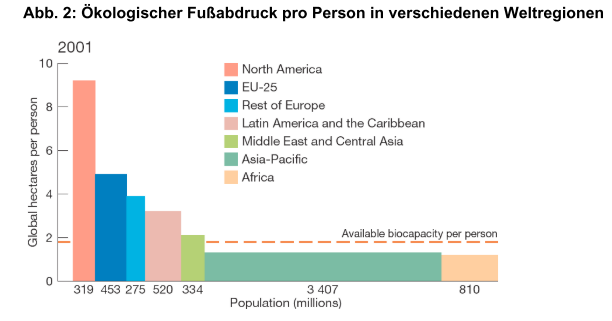
\includegraphics[width=12cm]{image_folder/oekFussabdruckWelt.png}
\caption{der ökologische Fußabdruck der Kontinente im Vergleich}
\label{fig:oekFussabdruckWelt}
\end{figure}

\begin{figure}[htbp]
\centering
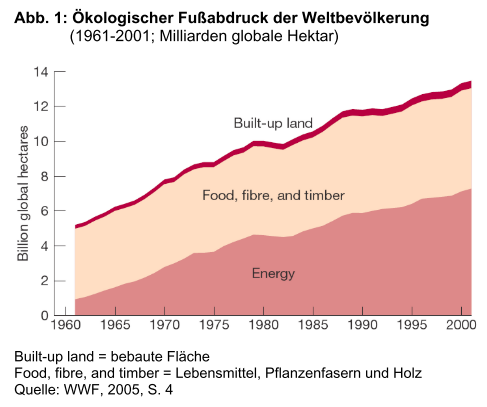
\includegraphics[width=12cm]{image_folder/oekFussabdruckZeit.png}
\caption{der ökologische Fußabdruck je nach Verwendung und Zeit}
\label{fig: oekFussabdruckZeit}
\end{figure}

\subsubsection{Komplexität von Nachhaltiger Entwicklung}

Schlussendlich stellen die zuvor genannten Bewertungsstrategien lediglich eine Annäherung oder einen Versuch zur Quantifizierung des Ressourcenverbrauchs dar. Der Unterschied besteht in der jeweiligen Fokussierung auf gewissen Parameter.  Als feste Berechnung können sie dabei nicht gewertet werden. Jedes der Konzepte auf seine Weise Lücken und Schwachstellen aufweist. Die Komplexität und viel des Begriff.<-- Fokussieren


Bei der Frage wie nachhaltige Entwicklung effizient und lösungsorientiert umgesetzt werden solle, stellen sich neben der Problematik der Verantwortlichkeit für die Verursachung der Umweltprobleme und die Gerechtigkeitfrage nach einer gerechten Verteilung der endlichen Ressourcen ("Global commons"). 
\begin{figure}[htbp]
\centering
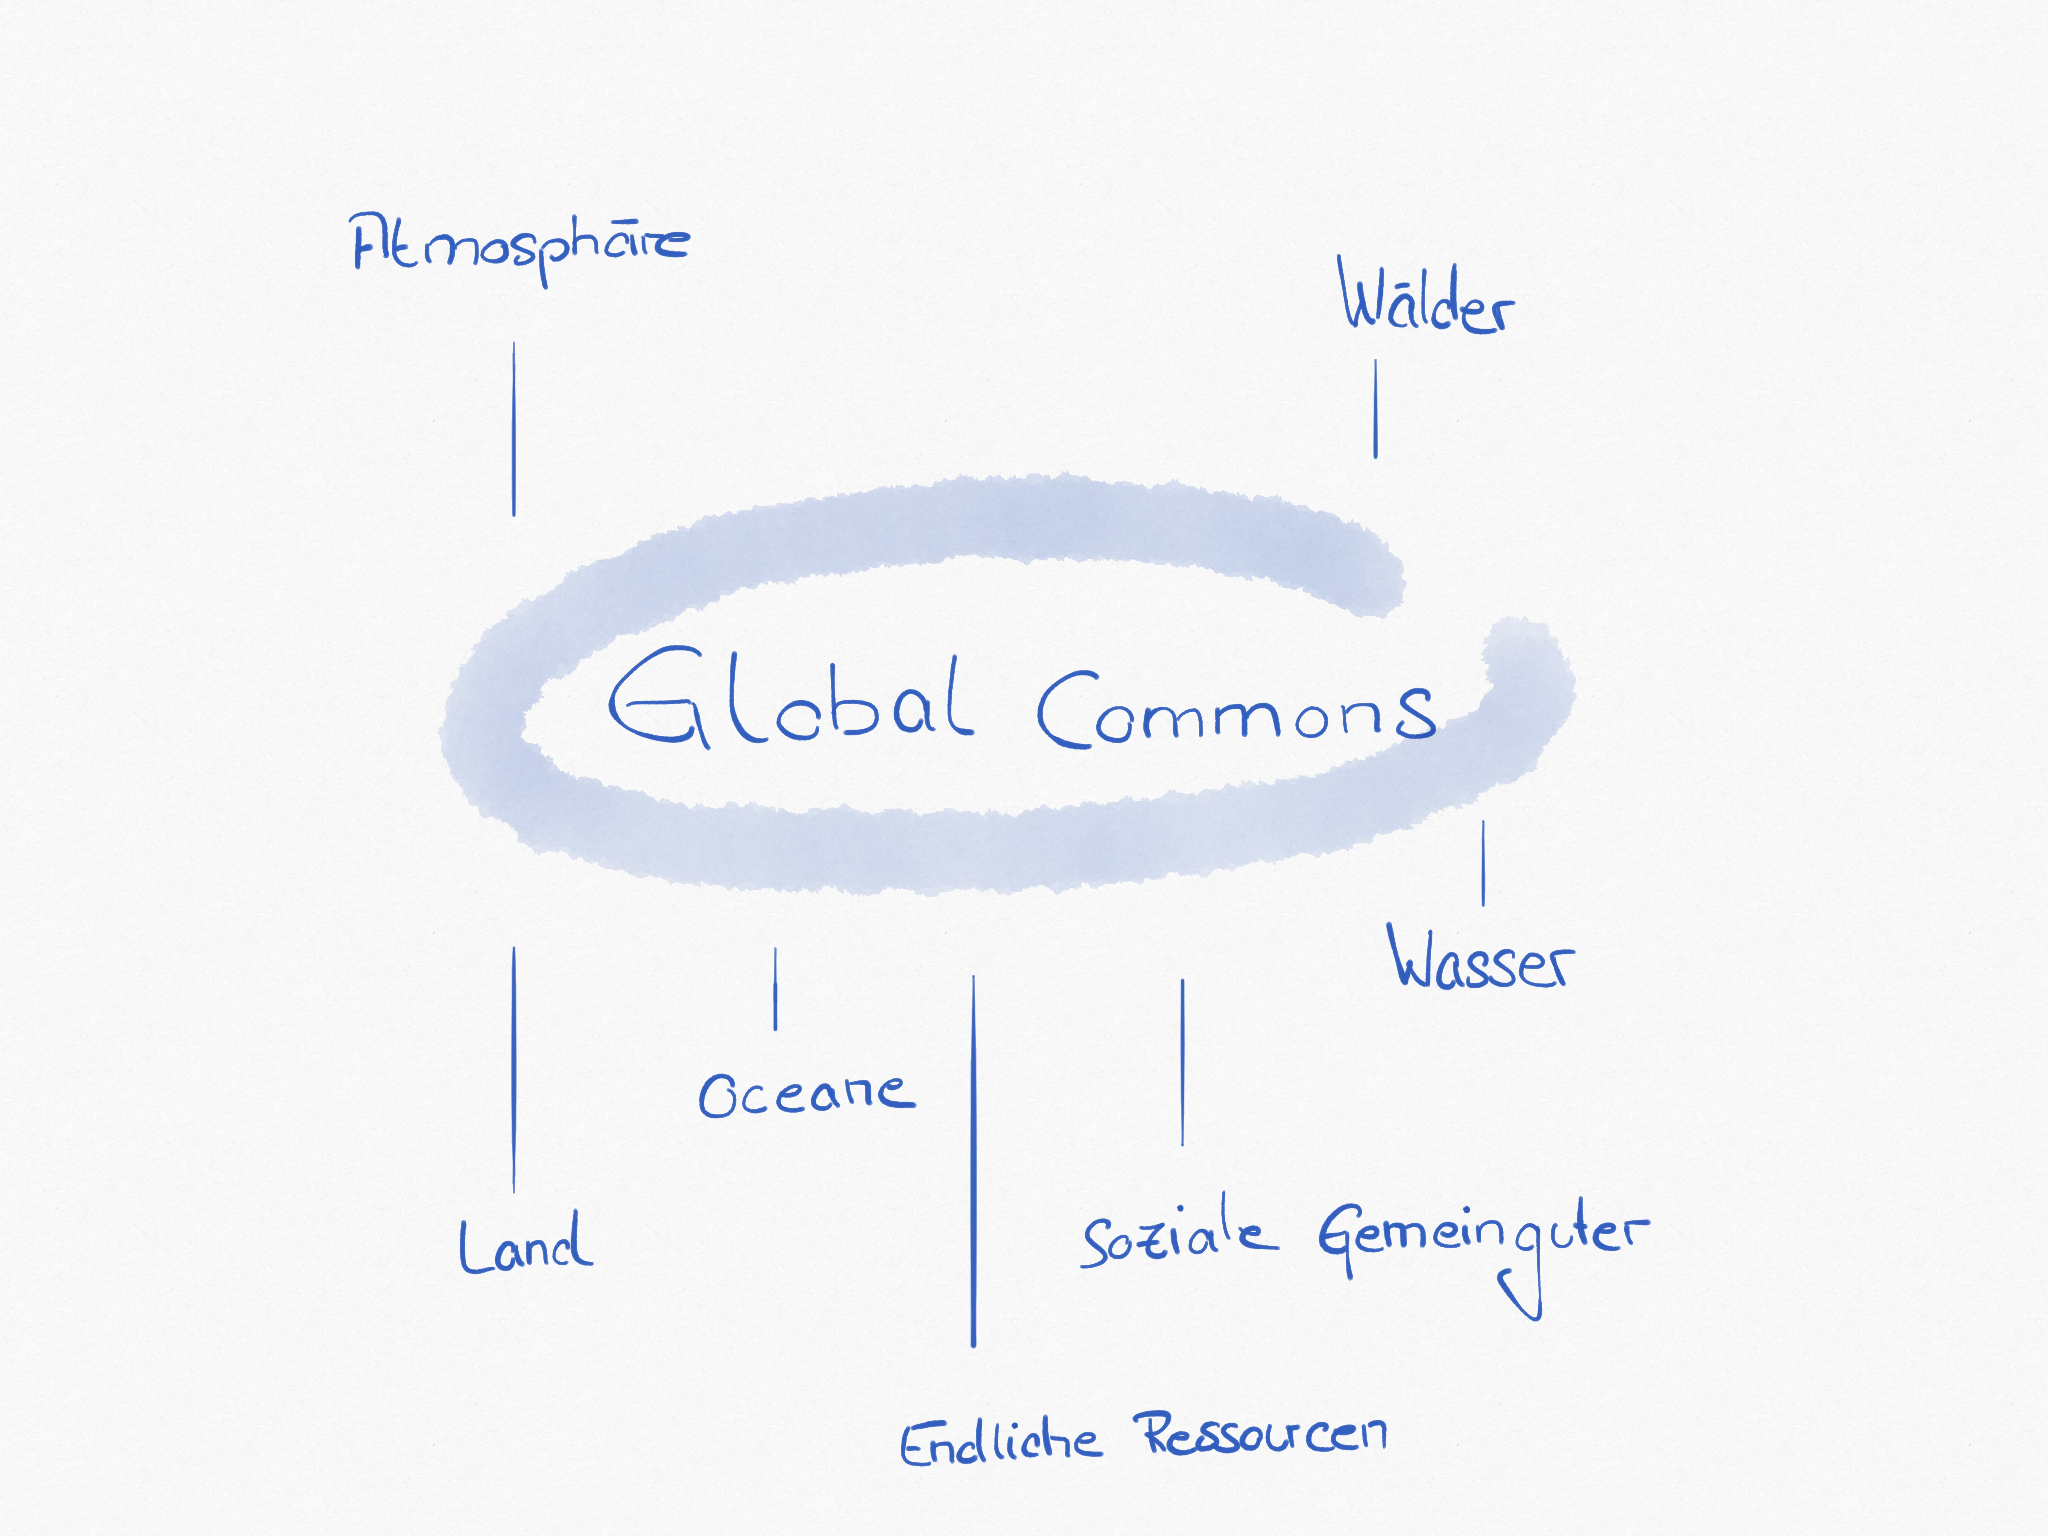
\includegraphics[width=14cm]{image_folder/globalcommons.png}
\caption{3-dim-Modell}
\label{fig: global commons}
\end{figure}

Nach dem Umweltgipfel\footnote{(UN-Konferenz für Umwelt und Entwicklung (UNCED, Erd-, Rio- oder Umweltgipfel) Nach diesem Gipfel gewann das Thema Nachhaltigkeit erstmals an weltweiter Relevanz). Beteiligt waren 178 Staaten. Zwar wurden auf dem Gipfel einige langrfistige Dokumente, wie die Klimarahmenkonvention, die Walderklärung, die Rio-Deklaration und die Agenda 21 unterzeichnet, so enthält keines der Dokumente überprüfbare Verpflichtungen. Dennoch ging von dieser Konferenz ein Impuls aus und der Begriff nachhaltigen Entwicklung („Sustainable Development”) ist seitdem Bestand von politischen Programmen.} im Jahr 1992 in Rio de Janeiro wurde diese Frage „von zahlreichen Kommentatoren so beantwortet, dass [...] jeder Mensch weltweit das gleiche Recht hat, die globalen Gemeinschaftsgüter in nachhaltiger Weise zu nutzen. Dieser Interpretation wird entgegengehalten, dass sie regional unterschiedliche Bedürftigkeiten und kulturelle Besonderheiten ignoriere.” \footcite{NachhaltigeBrockhaus.de} Ebenso besteht der "Einwand, dass neben den unterschiedlichen Bedürftigkeiten auch das unterschiedliche Leistungsvermögen berücksichtigt werden müsse."\footcite{NachhaltigeBrockhaus.de} Demnach sei das zulässige Nutzungsniveau eines Staates nicht nach der Größe seiner Bevölkerung, sondern nach seinem Beitrag zur globalen Wertschöpfung zu bestimmen."\footcite{NachhaltigeBrockhaus.de}

\begin{figure}[htbp]
\centering
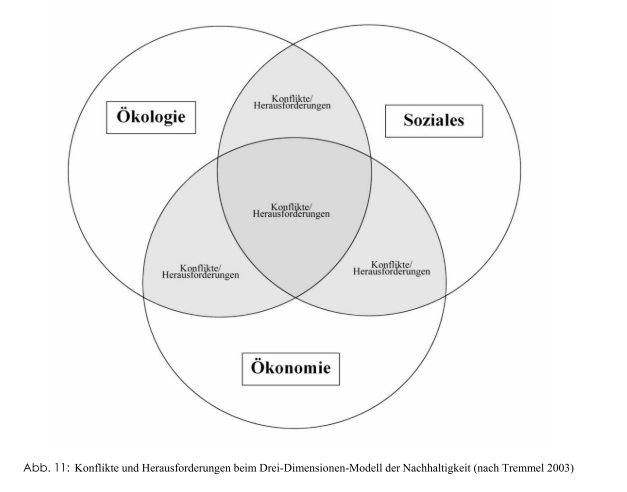
\includegraphics[width=10cm]{image_folder/dreidimensionenmodell_der_N.png}
\caption{3-dim-Modell}
\label{fig:3-dimensionen Modell}
\end{figure}

Konfliktpotenzial besteht ebenfalls bei der Priorisierung von Lösungsvorschlägen. Eine nachhaltige Lösung im sozialen Sinn kann sich auf Kosten von ökologischer Nachhaltigkeit auswirken und umgekehrt. Genauso kann auch eine Win-Win Situation entstehen. Ein Beispiel wäre hier ein urbanes Projekt zum Anbau von Gemüse, welches gleichzeitig die Stadtgemeinschaft fördert und der Verkauf des Projekts genug Einnahmen erbringt, dass die Gemeinde sich im folgenden Jahr weitere Arbeitsutensilien kaufen kann.

Entwicklungsländer stellen bei der Umsetzung bislang die sozialen und ökonomischen Aspekte in den Vordergrund. Da Industrienationen den Fokus auf die ökologische Dimension legen wird ihnen die Hauptlast bei der Lösung der bestehenden Probleme im ökologischen Bereich zugeschrieben. Industrieländern können ökologischen Aspekte in den Vordergrund, nicht zuletzt weil sie es sich finanziell leisten können. Da eine ökologisch nachhaltige Lebensweise aller Industrienationen, die Umweltschäden, welche in Schwellenländern entstehen nicht wettmachen können, und diese einen großen Anteil der weltweiten Bevölkerung und Fläche ausmachen werden gleichzeitig Lösungsinitativen von Seiten der Entwicklungsländer gefordert.

\begin{figure}[h]
\centering
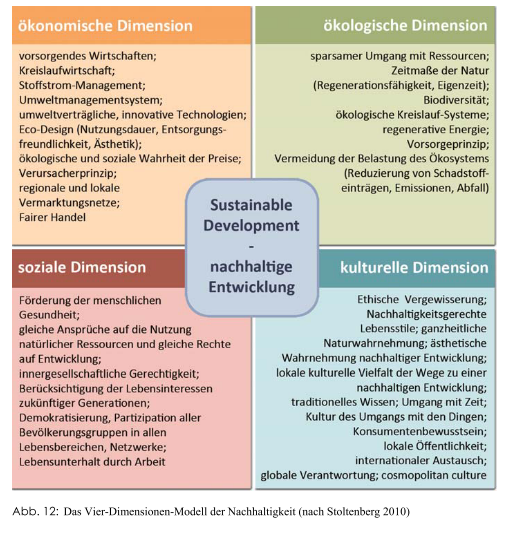
\includegraphics[width=6cm]{image_folder/vierdimensionenmodell_der_N.png}
\caption{4-dim-Modell}
\label{fig:4-dimensionen Modell}
\end{figure}




Um Projekte hinsichtlich ihrer Nachhaltigkeit ganzheitlich zu beurteilen, bedarf es viel Zeit und Recherche. Gleichzeitig muss bei der Untersuchung entschieden werden welche Dimensionen der Nachhaltigkeit primär betrachtet werden sollen, da wie bereits genannt, Projekte je nachdem unter welcher Brille der Nachhaltigkeit sie betrachtet werden unterschiedlich ausfallen.
\\
Im Rahmen dieser Forschungsarbeit soll bei der Bewertung die ökologischen Dimension von nachhaltiger Entwicklung im Vordergrund stehen. Aspekte der ökonomischen Dimension können unter Umständen mit einfließen, da diese Faktoren sich häufig gegenseitig bedingen. Soziale und kulturelle Kriterien werden in dieser Forschungsarbeit nicht betrachtet, da dies den Rahmen dieser Forschungsarbeit sprengen würde.

Aus den zuvor genannten Methoden zur Bewertung von Nachhaltigkeit wurden für diese Forschungsarbeit folgende Kriterien ausgewählt, hinsichtlich welcher Projekte bewertet werden sollen.

\begin{itemize}

\item 1. Schutz der Umwelt (natürlichen Ressourcen: v.A Boden, Wasser, \item Luft (Vermeidung der Belastung))
\item 2. Nutzung regenerativer Energie
\item 3. sparsamer Umgang mit Ressourcen (von Anbau bis Konsum)
\item 4. Reduzierung von Schadstoff, (Emission, Abfall, Pestizide)
\item 5. Kreislaufsystem
\item 6. Biodiversität
\item 7. Dritte und weitere Umweltbedingungen
\item 8. Bedachte Regenerationszeit der Natur
\item 9. ökonomische Wirtschaftlichkeit
\item 10. Langfristigkeit
\item 11. (Gesellschaftliche und politische Akzeptanz)
\end{itemize}

\subsubsection{Kritik am Begriff der Nachhaltigkeit}\footcite{NachhaltigeBrockhaus.de}
Die übermäßige Verwendung des Begriff Nachhaltigkeit in der Wirtschaft und Politik hat bei vielen Bürgern zu Misstrauen geführt. Kritisiert wird vor allem, dass der Begriff überladen sei und als Sammelbegriff für alles Gute genannt werde, was unerfüllbare Erwartungen wecke. Gleichzeitig sei der Begriff beliebig geworden: “Unter der Flagge der nachhaltigen Entwicklung könne man trotzdem für komplett gegensätzliche Dinge eintreten.” So entstände die Meinung, Nachhaltigkeit sei inhaltslos und habe nur rhetorische Funktionen, was die Leitbildfähigkeit des Begriffs außer Kraft setze. Noch schärfer sind Stimmen, die Nachhaltigkeit von vornherein als utopisch und Illusion bezeichnen.
\\
Es darf geschlussfolgert werden, dass aufgrund dieser Unsicherheit hinsichtlich des eigenen Verhalten und der zukünftigen Entwicklung der Umwelt eine große Frustration bei der Bevölkerung entstanden ist. Und es entsteht die Frage, welche Lösungsansätze zu einer nachhaltigen Entwicklung der Welt beitragen.  


\subsubsection{Nachhaltigkeitswissenschaften}
Allgemein lässt sich festhalten, dass sich die „Nachhaltigkeitsforschung [...] mit Problemen, die die langfristige Sicherung der gesellschaftlichen Entwicklungsbedingungen gefährden” befasst.\footcite[S.126]{MichelsenGrundlagenEntwicklung}
Ihre Anfänge hatte die Nachhaltigkeitswissenschaft im Rahmen der Forschung zum Globalen Wandel in den späten 1980er Jahren. Laut der Autoren des..  gab unter anderem die Publikation „Die Grenzen des Wachstums“ von Meadows et al. 1972 den Anstoß zur Forschung bezüglich der Frage der globalen Umweltprobleme.
Drei internationale Großforschungsprogramme werden bezüglich der Nachhaltigkeitswissenschaften insbesondere genannt: (1) das „International Geosphere-Biosphere Programme (IGBP)“, (2) das „World Climate Research Programme“ und (3) das
„International Research Programme on Biodiversity (DIVERSITAS)“. In Deutschland kann man heute Nachhaltigkeitswissenschaften an mehr als 15 Städten als eigenständigen Studiengang oder als integrationsmodul studieren.


\begin{figure}[h]
\centering
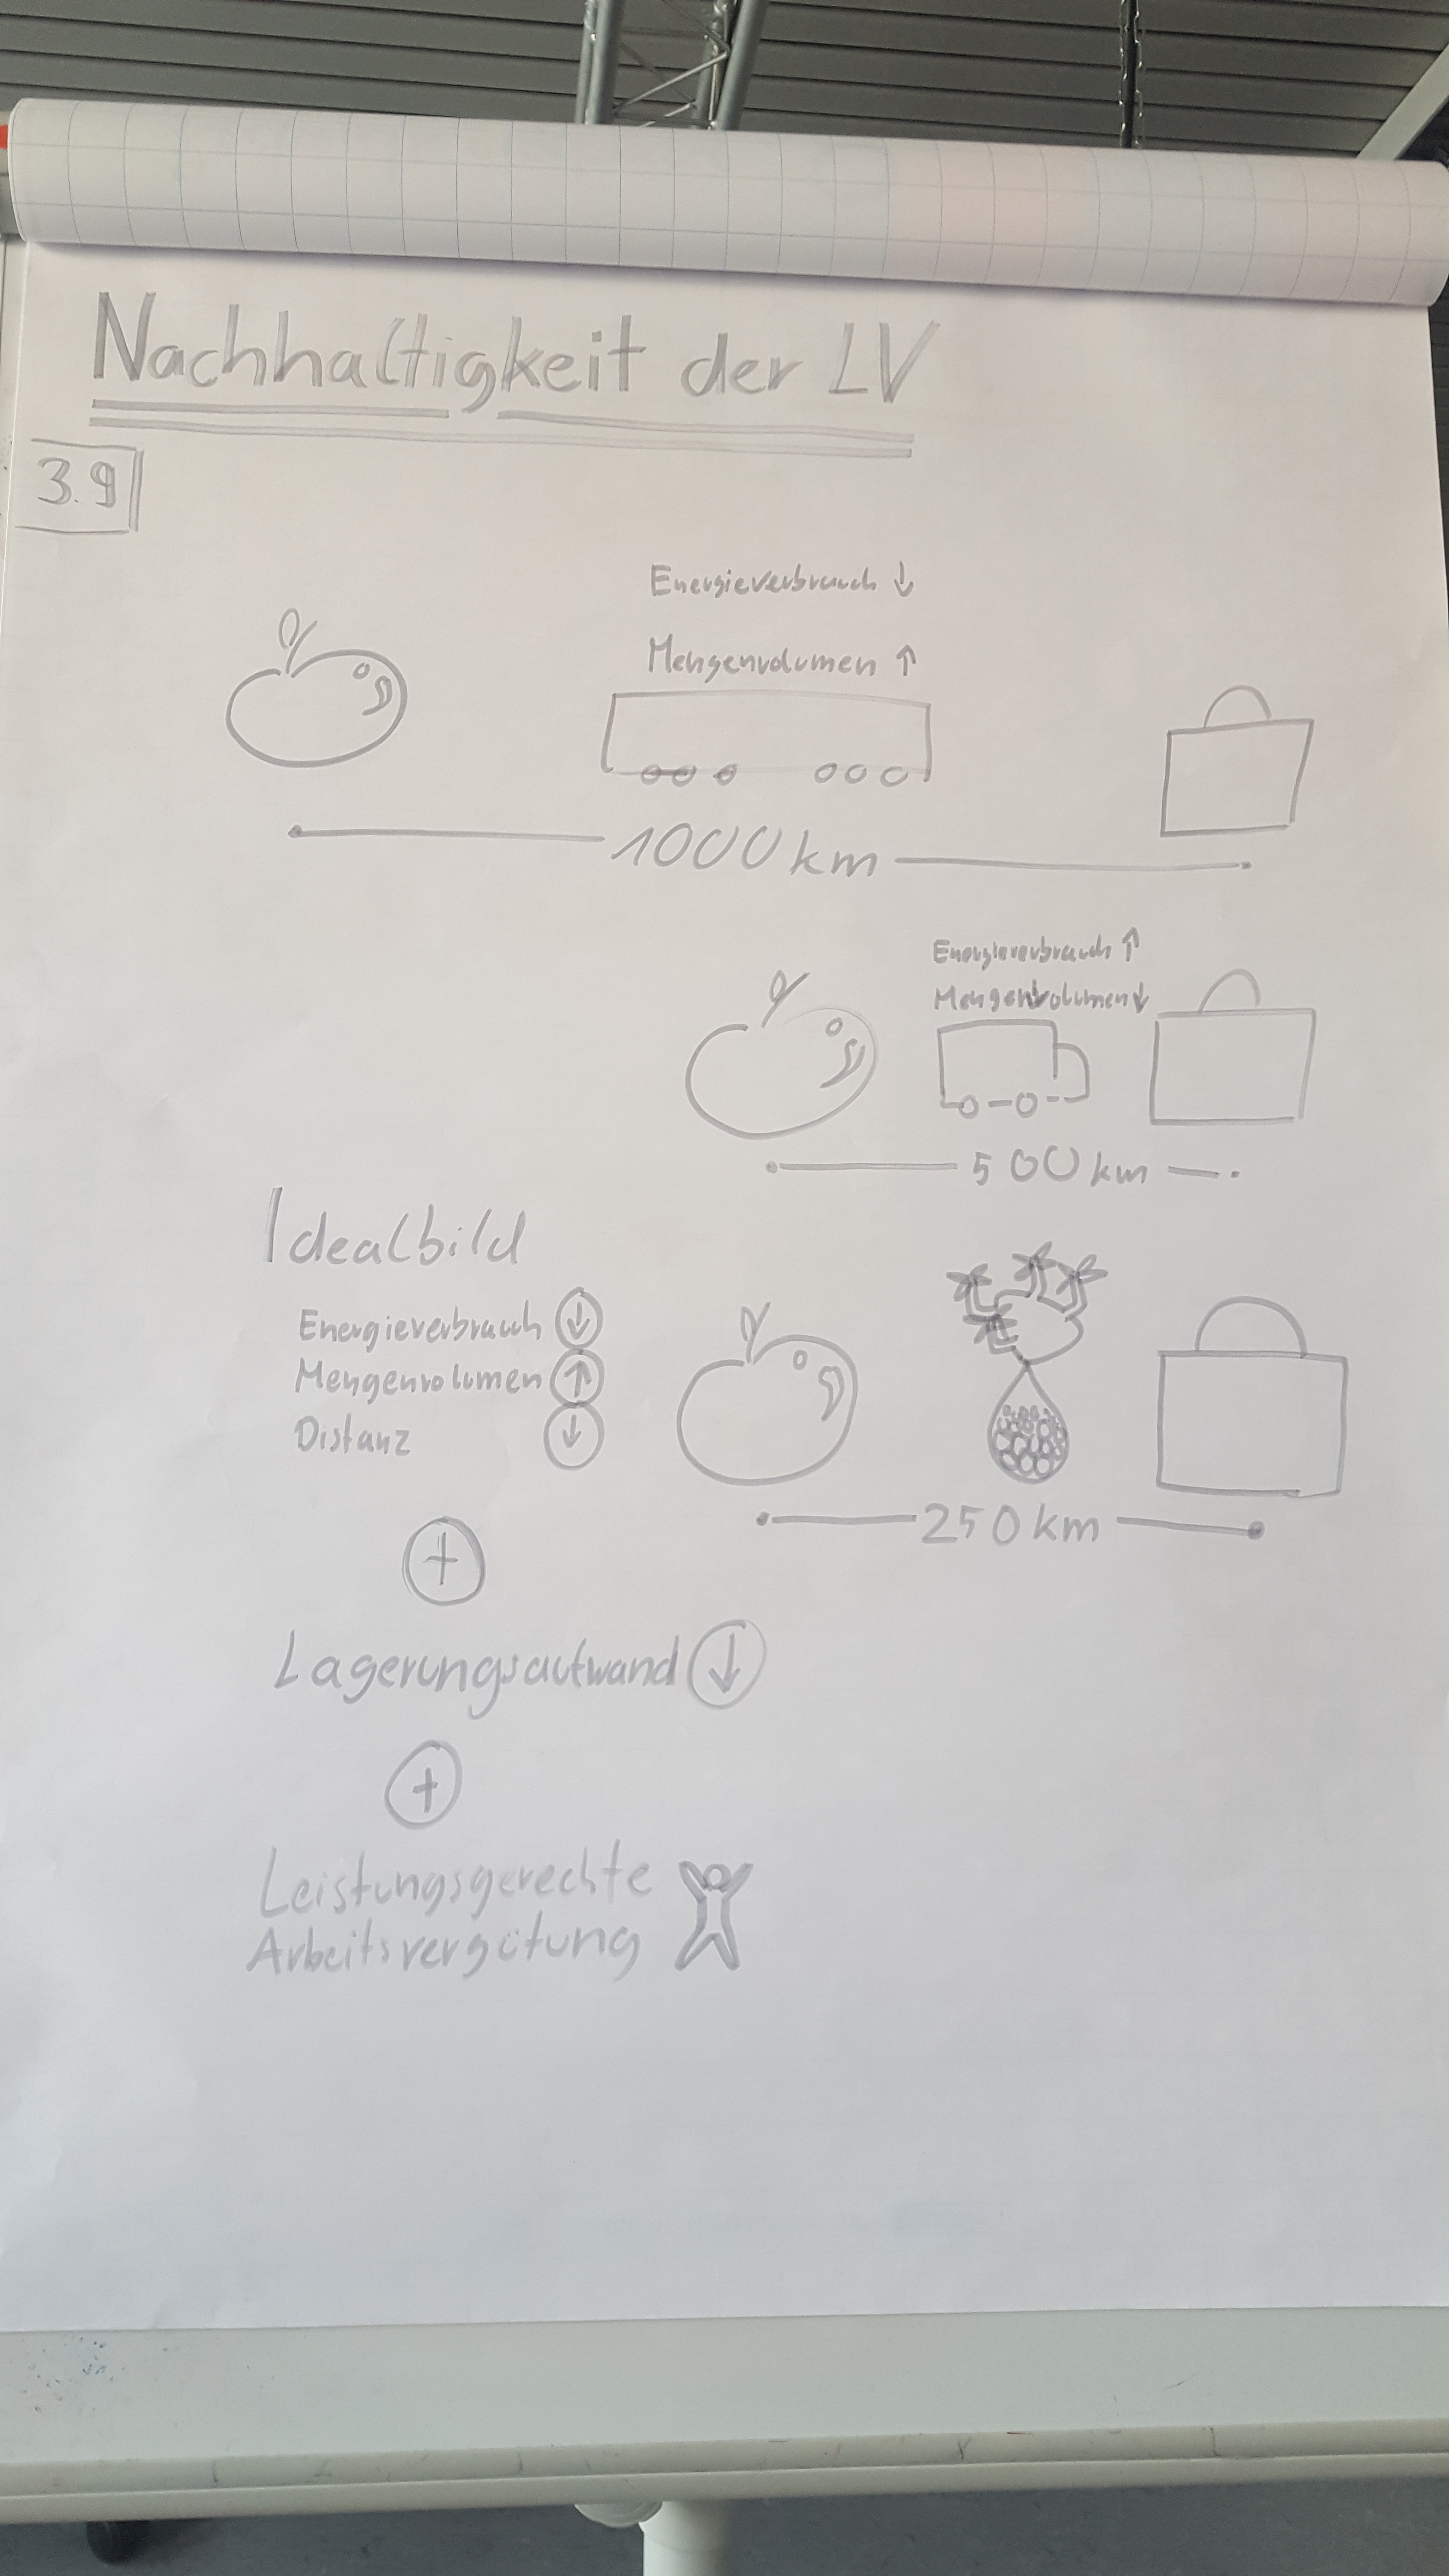
\includegraphics[width=5cm]{image_folder/skizze1.jpg}
\caption{Nachhaltigkeit der LV}
\label{fig:Skizze_Nachhaltigkeit}
\end{figure}

\FloatBarrier

\section{Die Distanz zwischen Stadtbevölkerung und Landwirtschaft}
\subsection{Verstädterung im Hinblick auf die Lebensmittelversorgung***}
Wie Städte entstanden sind und sich bis heute ausbreiten hat viel damit zu tun wie Menschen das Problem der Nahrungsmittelsicherung lösten. Elmquist, Redman, Barthel und Costanza beschreiben in „Urbanization, Biodiversity and Ecosystem Services: Challenges and Opportunities“ hierzu drei vergangene Lösungsansätze, an dem sich dieses Kapitel anlehnt.\footcite[S.14ff]{Elmqvist2013} 
\\
\\ 
Der erste Ansatz war das Nomadentum. Menschen zogen von Gegend zu Gegend, um sich zu ernähren. Sie folgten Tierherden sowie klimatisch günstigeren Regionen, wo nahrhafte Rohstoffe zu finden waren. Der zweite Ansatz war die Domestizierung von Tieren und Pflanzen. D.h. Rohstoffe wurden passend nach Bedarf herangezüchtet, geerntet und wieder angebaut. Menschen waren dadurch weniger wechselnden Bedingungen ausgesetzt und verbesserten stetig ihre Nahrungsmittelerzeugung. Das erlaubte dauerhafte Sesshaftigkeit und förderte eine sichere Existenzgrundlage. Aus diesem Grund setzten sich kleine ländliche Gemeinden zur verbreitetesten Siedlungsform auf der Erde durch. Sie waren zwar unabhängig und isoliert voneinander, zeichneten sich allerdings als besonders widerstandsfähig gegenüber dem vorherigen Lebensstil aus. Für Elmquist et. al. war es also keine Überraschung, dass die Bevölkerungszahl dadurch anstieg. Darüber hinaus wuchsen ländliche Gemeinden derart, dass die Menge an Menschen überschüssig zur nötigen Arbeit auf dem Acker war. \\
\\
Den Höhepunkt dieses Prozesses bildete 5500 v.C. die erste städtische Siedlung in Mesopotamien - der dritte Ansatz. Die dortigen Innovationen wie das Schreiben, Monumentalbauten oder vertiefende Handwerkskünste zeigten das Potenzial dieser neuen Siedlungsform. Die Autoren bezeichnen Städte als Zentren der Innovation. Verglichen mit ländlichen Gemeinden zeichnet sich eine Stadt durch eine äußerst diverse und voneinander abhängige Gemeinschaft aus. Ländliche Gemeinden sind zwar unabhängiger und selbstversorgend, dafür war das Wachstum dieser Siedlungsform begrenzt. Anders verhält es sich mit Städten. Bezüglich der Versorgung war eine Stadt auf die umliegenden Gemeinden angewiesen. Jedoch trug der Austausch von Waren, technologischen Erfindungen sowie wissenschaftliche Erneuerungen enorm zum Wachstum und der Verbreitung von Städten bei. Hinzu kam, dass eine soziale Erneuerung nötig war um diese große Gruppe von Menschen und groß skalierte produktive Aktivitäten zu organisieren. Eine klassenstrukturierte Gesellschaft, eine formalisierte Rechtsgrundlage und eine territoriumsbasierte Regierung bildeten daher den charakteristischen Rahmen. Damit eine Gemeinschaft auf diesem dichten Lebensraum funktionierte, war nämlich eine gewisse Ordnung im Miteinander erforderlich. Diese Siedlungsform erwies sich so erfolgreich, dass viele Städte Wohlstand und Sicherheit genossen. 
\\
\\
Der wachsende Wohlstand in Städten führte zu regelmäßigen militärischen Angriffen. Zum Schutz wurden daher Stadtmauern gebaut. Diese Sicherheitsmaßnahme wiederum förderte die Produktivität und damit den Wohlstand. Das wiederum führte zu einer wachsenden Bevölkerung und durch die Eingrenzung zu einem dichteren Wohngefüge, das kennzeichnend für viele heutige Städte ist. Der erfoderliche Anbau an Rohstoffen fand daher meistens im Umland statt und weitere Arbeitskräfte auf dem Land siedelten nahe der Stadt. \\
\\
Trotz der Tatsache, dass Städte unterschiedlich entstanden sind, sehen Elmquist et. al. folgende Gemeinsamkeit:\footcite[Vgl.][S.19ff]{Elmqvist2013} Diese Anhäufung von Menschen in einer Stadt führte zur Spezialisierung von diversen Beschäftigungen. Dies hatte zur Folge, dass der Großteil der urbanen Bevölkerung immer weniger selbstversorgende Tätigkeiten ausübte. Dadurch wurde einem großen Anteil der ruralen Bevölkerung die Verantwortung übertragen so viele Nahrungsmittel zu produzieren, dass sie sowohl sich selbst als auch die Stadtbevölkerung versorgen konnten und gleichzeitig ausreichend Gewinn machten um die Verteilung und den Transport dieser Güter zu decken. Sie übernahmen demnach die Rolle des Versorgens in diesem Stadt-Land-System. Das war eine große Last im Vergleich zur blosen alleinigen Versorgung. Auch als die sozialen Rollen der urbanen und ruralen Bevölkerung auseinanderdrifteten änderten sich die jeweiligen Ziele und Verständnisse zur Landwirtschaft. Dementsprechend ging es um die maximale Produktion auf Kosten der regenerativen Kapazitäten der natürlichen Ressourcen. Elmquist spricht hier von  „ [...] maximizing short-term returns with little concern for long-term consequences.“\footcite[S.20]{Elmqvist2013}
%------------

\begin{figure}[h]
\centering
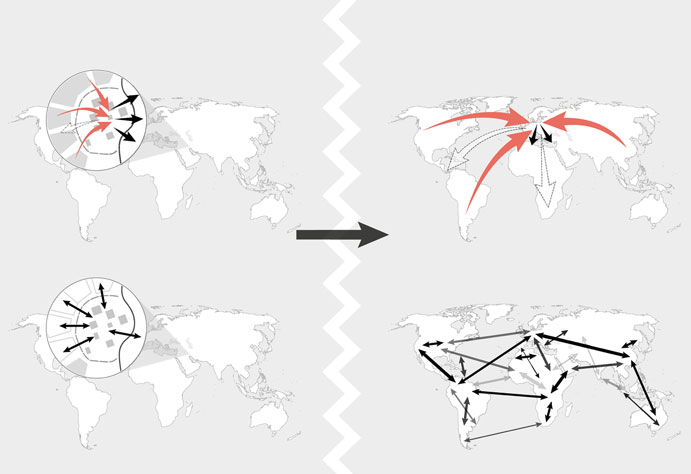
\includegraphics[width=12cm]{image_folder/connections_1.jpg}
\caption{Früher war die Versorgung der Städte abhängig vom Umland, mit einem direkten Austausch. Heute hingegen hat sich eine globale Abhängigkeit mit komplexen Lieferketten entwickelt.}
\label{fig:verbindungen}
\end{figure}

Zusammenfassend lässt sich sagen, dass Städte bereits seit ihrer Existenz eine abhängige Beziehung zu ländlichen Gemeinden haben. Denn der Überschuss in der Landwirtschaft sorgte erst dafür, dass diese Siedlungsform entstehen konnte. Städte sind zwar globale bzw. regionale Zentren der Innovation und Administration, waren aber seit Anbeginn angewiesen auf die Einfuhr von Ressourcen. 

\subsection{Entwicklung globaler Ernährungssysteme}
In diesem Kapitel wird die Gewichtung von lokalen Städten auf die globale Perspektive zur Lebensmittelversorgung gewechselt, um ein tieferes Verständnis über die beiden Komponenten zu erhalten.
\\
\\
Wie es zur Entwicklung der aktuellen globalen Lebensmittelversorgung gekommen ist, teilen Friedmann und McMichael in drei Phasen auf. Diese Phasen bezeichnen sie als sogenannte Lebensmittelregime, ein Konzeptrahmen das zur Untersuchung dient welche internationalen Verbindungen zur Lebensmittelproduktion im Zeitraum kapitalistischer Transformation vorherrschten.\footcite[Vgl.][S.95]{Friedmann1989AGRICULTUREPresent}

\subsubsection*{Anfänge nationalen Handels}
Das erste Lebensmittelregime umfasste die Zeit 1870 - 1914. Das sei einerseits der Höhepunkt der Kolonisation und andererseits die Entwicklung von Nationalstaaten. Die besiedelten Kolonien (wie Australien, Kanada, Neu Seeland und die Vereinigten Staaten), europäische Kolonialmächte und die beherrschten Kolonien (wie zum Beispiel Indien) waren demnach die maßgebenden Akteure in dieser Zeit. Durch neue Technologien war das Ernährungssystem über mehrere Kontinente erst möglich. Züge gewährleisteten den Transport großer Mengen an Rohstoffen. Wesentlich in dieser Zeit sei der Import von Getreide und Fleisch nach Europa und im Gegenzug die Lieferung von hergestellten Waren, Arbeit und Kapital. Der Anreiz nach Beschäftigung ließ viele europäische Familien in diese Siedlerstaaten ziehen. Das förderte die verlagerte landwirtschaftliche Produktion in den Siedlerstaaten, was sowohl dem Bedarf an Nahrungsmitteln und dem Platzmangel in den europäischen Staaten in mehreren Gesichtspunkten entgegen kam. Auch durch das günstige Klima und die billige Arbeitskraft konnten sie landwirtschaftliche Produkte preiswerter herstellen, als es im eigenen Land möglich war. Desweiteren optimierten landwirtschaftliche Erfindungen wie Dünger und Maschinen die Ernte. Die Handelsbeziehungen zwischen den Siedlerstaaten und Europa sei die Basis eines ersten internationalen Handelssystems. Friedmann et. al. zufolge führten die Importe von Getreide und Fleisch von Siedlerstaaten und der Export von Kapital und Menschen um jene Lebensmittelproduktionen zu organisieren zum industriellen Kapitalismus.\footcite[Vgl.][S.96ff]{Friedmann1989AGRICULTUREPresent}


\subsubsection*{Nationaler Austausch von Gütern}
Friedmann et. al. zweites Regime beinhalte das Ende des zweiten Weltkrieges bis etwa 1970. Den Autoren zufolge waren nach dem zweiten Weltkrieg die Vereinigten Staaten von politischem Interesse getrieben, ihren Export an Lebensmitteln auszubauen. Im Anbruch des kalten Krieges wollten sie die Industrialisierung in Entwicklungsländern und in Europa vorantreiben. Durch die Subvention ihrer heimischen Landwirtschaft sorgten sie zu Produktionsüberschüssen von Getreide und Mais, was sie zum einen als Hilfspaket an europäische Staaten schickten und preiswert an Entwicklungsländer anboten. Gleichzeitig beschränkten sie den Import von ausländischem Getreide. Das hatte zur Folge, dass in den Entwicklungsländern eigene Lebensmittel verdrängt wurden und diese abhängig vom Export waren. Desweiteren wurde der Preis tropischer Rohstoffe aus diesen Ländern gering gehalten, was das Ungleichgewicht in dieser Handelbeziehung verstärkte. Ein weiterer wesentlicher Aspekt in dieser Zeit war der Wandel zur Massenproduktion in Form von intensiver Tierhaltung und der Herstellung haltbarer Lebensmittel in den sechziger Jahren. Landwirte in den Industriestaaten wechselten ihre Rolle vom Lebensmittelproduzent zum Lieferant eines Rohstoffes. Auch ihr Kundenkreis verlagerte sich vom Endverbraucher zu großen Firmen. Das Ende dieser Phase kündigte sich an als zum einen europäische Staaten sich zu starken Lebensmittelexporteuren entwickelten und dem amerikanischen Export Konkurrenz machte. Zum anderen stärkten Entwicklungsländer ihre heimische Agrarwirtschaft und schränkten Exporte ein. Dadurch waren Industriestaaten plötzlich angewiesen auf Importeure, die ihre Überschüsse abnahmen.\footcite[Vgl.][S.103ff]{Friedmann1989AGRICULTUREPresent}

\subsubsection*{Globalisierung der Lebensmittelproduktion}
Das dritte Lebensmittelregime sei geprägt von einer Globalisierung der Lebensmittelindustrie. Die Lebensmittelproduktion, ihre politische Förderung und Regulation, biochemische Innovationen, die standortunabhängige Produktionen ermöglichen als auch der Verkauf geht über nationale Grenzen hinweg. Stierrand spricht hier von der Bedeutung „transnationaler Firmen“ als auch die „Internationalisierung von Konsummustern und des Geschmacks verbreitet durch Massenmedien“\footcites[Vgl.][S.24ff]{Stierand2008StadtLebensmittel}, die sich in Angebot und Nachfrage ergänzen. Im Hinblick auf die Rolle der Landwirte äußert sich der Autor folgendermaßen:
\begin{displayquote}
„Mit der Veränderung des weltweiten Ernährungssystems haben sich die Schwerpunkte und die Machtstrukturen innerhalb des weltweiten Ernährungssystems verlagert. [...] Mit sinkendem Anteil der Landwirte an der Produktion von Lebensmitteln, gewannen andere Akteure größere Anteile der Wertschöpfung und Macht. Dabei hat der Profit in der Landwirtschaft noch nie einen wichtigen Anteil am nationalen Einkommen eingenommen. Ihre Funktion für die nationale Ökonomie war und ist die Bereitstellung von billigen Lebensmitteln, so dass der Anteil am Lohn, der nicht für weitergehenden Konsum zur Verfügung steht, möglichst gering ist.“\footcite[S.25]{Stierand2008StadtLebensmittel}
\end{displayquote}

Abschließend sind aus den Kapiteln 6.1. und 6.2. folgende Merkmale zu erkennen: Im allgemeinen lösten sich Menschen von der lokalen Selbstversorgung zur globalen Fremdversorgung. Die Distanz zwischen Stadtbewohnern - den Konsumenten - und Landwirten erhöhte sich im sozialen Sinne durch die Anreihung von weiteren Akteuren in der Produktionskette und physisch durch die vielfältige geographische Verteilung der Produktions- und Vertriebsstätten. Waren die versorgende Bevölkerung meistens noch im Umland von Städten positioniert, erschwert es die aktuelle Komplexität des Ernährungssystems diese nachzuvollziehen. Folgt man Stierrands obiger Aussage, erkennt man auch die die Distanz zwischen Konsumenten und Landwirten anhand der wirtschaftlich geringen Wertschätzung. 


\section{Aspekt der Romantik und „Landlust“ in Bezug auf Urbaner Landwirtschaft am Beispiel Deutschland}

\subsection{Aufkommen der Landlust“ und deren Formen}
Eine romantische Vorstellung des Landlebens und der Landwirtschaft bei der Begrünung von Städten ist ein weit verbreitetes Phänomen und dazu nicht neu. Wie zuvor beschrieben trat dieses Phänomen in der Vergangenheit häufiger auf. Da Landwirtschaft bis zur Phase der Industrialisierung auch in der Stadt oder im städtischen Umland stattfand und die Versorgung so durch eigens angebaute Lebensmittel in der Subsitenzwirtschaft bewerkstelligt wurde, bildete diese „ursprüngliche“ Form der Landwirtschaft in Deutschland und auch global gesehen die Tradition der Nahrungsmittelversorgung ab. Erst mit der Verdichtung der Städte und der Umwandlung von einer Agrar- zur Industriegesellschafft verschwanden die städtischen Gärten und Landwirtschaftsflächen. Dieser Gesellschaftsumschwung führte dann zur Urbanisierung. \footcite[Vgl.][S. 32ff]{Egnolff2015DieIdeal}\\
\\
Enge Wohnverhältnisse, schlechte Hygiene und niedrige Lebensstandards im Zuge dieser führten zur aufkommenden „Landlust“ und der Rückbesinnung auf ländliche Freiräume. Die „Landlust“ in Deutschland, welche in der folgenden Arbeit durch das Verlangen nach einem natürlichem und ländlichen Lebensstil definiert wird, äußerte sich dann beispielsweise in der Romantisierung des Landlebens und der Großstadtkritik außerdem im UG, im Konzept der Gartenstadt-, die Siedlungs- und die Kommunenbewegung sowie im Kleingartenwesen. Diese Bewegungen sollten einen Gegensatz zur Industriewirtschaft und der damaligen Politik vom letzten drittel des 19. Jahrhunderts bis zum ersten Weltkrieg bilden.\footcite[Vgl.][S. 35]{Egnolff2015DieIdeal}\\
\\
Hinter den Siedlungs- und Kommunenbewegungen stand die Idee einer Gemeinschaft die soziale und ökonomische Gleichheit sowie körperliche und geistige Gesundheit anstrebten. Hierzu diente das Landleben und die damit verbundene Rückbesinnung als Strebensziel. Die Romantisierung des Landlebens aus Sicht der Stadtbevölkerung als Raum für das gesunde Leben in Freiheit und Idylle ging aus dem Wunsch nach dem Gegenteil zum weniger natürlichen Stadtleben hervor. Diese Bestrebungen mündeten dann in die Gartenstadtbewegung welche die Misstände in der Stadtbevölkerung durch die Planung von Gartenstädten im Umkreis abfangen wollte. Die Gartenstädte sollten ein Zusammenspiel von Stadt und Land bieten welches die Lebensbedingungen der Einwohner verbessern sollte. Diese Idee geht wiederum auf Ebenezer Howard zurück welcher 1889 in seinem Werk „Garden Cities of To-morrow“ (ursprünglich „Tomorrow: A Peaceful Path to Real Reform“) dieses Konzept beschreibt. Die erhofften Entwicklungen fanden dennoch nicht im entsprechenden Ausmaß statt.\footcite[Vgl.][S. 36]{Egnolff2015DieIdeal}

\begin{displayquote}
„Die tatsächliche Umsetzung der Gartenstadt fand jedoch in suburbanen Gebieten und nicht als Verknüpfung von Stadt und Land statt. Die erhofften gesellschaftlichen Veränderungen blieben aus und die Bilanz der Wohnungsstatistiken der Gartenstadt-Gesellschaften war insgesamt niedrig“\footcite[S. 36]{Egnolff2015DieIdeal} 
\end{displayquote}


Kleingärten finden auch heute noch Platz in Städten. Das Bundeskleingartengesetz definiert Kleingärten „zur nichterwerbsmäßigen, gärtnerischen Nutzung, insbesondere zur Gewinnung von Gartenbauerzeugnissen und zur Erholung“\footcite[§ 1]{Verbraucherschutz2006BundeskleingartengesetzBKleingG}

Das Kleingartenwesen entwickelte sich aus der Reaktion gegen beengte und unhygienische Wohnverhältnisse heraus. 

\begin{displayquote}
„Die Gärten sollten als Ausgleich zum Arbeitsalltag und zur Selbstversorgung dienen und den Bevölkerungsgruppen, die aus ländlichen Gegenden zuwanderten, die Eingliederung in die urbane Gesellschaft erleichtern. Zusätzlich sollten sie der Entfremdung des Menschen von der Natur, die mit der Industrialisierung
und Urbanisierung auftrat, entgegenwirken.“ \footcite[Vgl.][S. 38]{Egnolff2015DieIdeal}
\end{displayquote} 

Die Gründung des ersten Schrebergartens ging auf Ernst Innocenz Hauschild zurück der diesen als Spielplatzinitiative erdachte. \footcite[Vgl.][S. 39]{Egnolff2015DieIdeal}


Es lässt sich feststellen, dass die Landlust besonders stark in städtischen Siedlungen ausgeprägt ist. Dies hängt zum einem mit der fehlenden Ruhe und Idylle wie auch mit dem Bedürfnis nach freier Entfaltung in "gesunder Umgebung" zusammen. Im Zuge der Urbanisierung ziehen die vermeintlichen Vorteile der Stadt nach wie vor Landbewohner in verdichtete Gebiete. Die Erwähnte Vorteile sind überweigend: 

\begin{itemize}
\item bessere Infrastruktur
\item mehr Abwechslung
\item mehr Erfahrungsmöglichkeiten 
\item mehr soziale Begegnungen
\item ein größeres Angebot von Arbeitsplätzen
\item mehr Konsummöglichkeiten
\end{itemize}

Die wahrgenommenen Nachteile sind oft die Belastungen im Zusammenhang mit dem Verkehr und die schwierige Wohnungssituation.\footcite[S. 41]{Egnolff2015DieIdeal} Trotz der Vorteile glaubt die Mehrheit der deutschen dass das Leben auf dem Land qualitativ hochwertiger sei. Dies liegt oft an einer übertriebenen Wahrnehmung für das ländliche Leben.

Eine 2014 durchgeführte Umfrage des Allensbach Institus für Demoskopie zur „Sehnsucht der Stadtbewohner nach Ländlichkeit“ belegte den Trend der Landlust. So sind 40\% der Befragten der Meinung, dass das Leben auf dem Land lebenswerter sei.\footcite[Vgl.][S. 15 Abb.2]{Dr.ThomasPetersen2014DieLandlichkeit}


Die Vorteile für das Land seien demnach:

\begin{itemize}
    \item Gesundheit
    \item Natürlichkeit
    \item gute Luft
    \item Nachbarschaftshilfe
    \item günstiger Wohnraum
\end{itemize}

Interessant ist, dass 27 Prozent der 1520 Befragten die Assoziation „einsam“ dem Landleben, aber zu 39 Prozent dem Leben in der Stadt zuordnen. Laut Dr. Petersen handele es sich hierbei um ein Klischee demnach Menschen in der anonymen Großstadt vereinsamen. Dieses Klischeebild hätte sich in der Umfrageforschung über Jahrzehnte hinweg jedoch nie bestätigen lassen. Dennoch halte sich das Klischee bis heute hartnäckig.\footcite[Vgl.][S. 7ff]{Dr.ThomasPetersen2014DieLandlichkeit}

\begin{figure}[htbp]
\centering
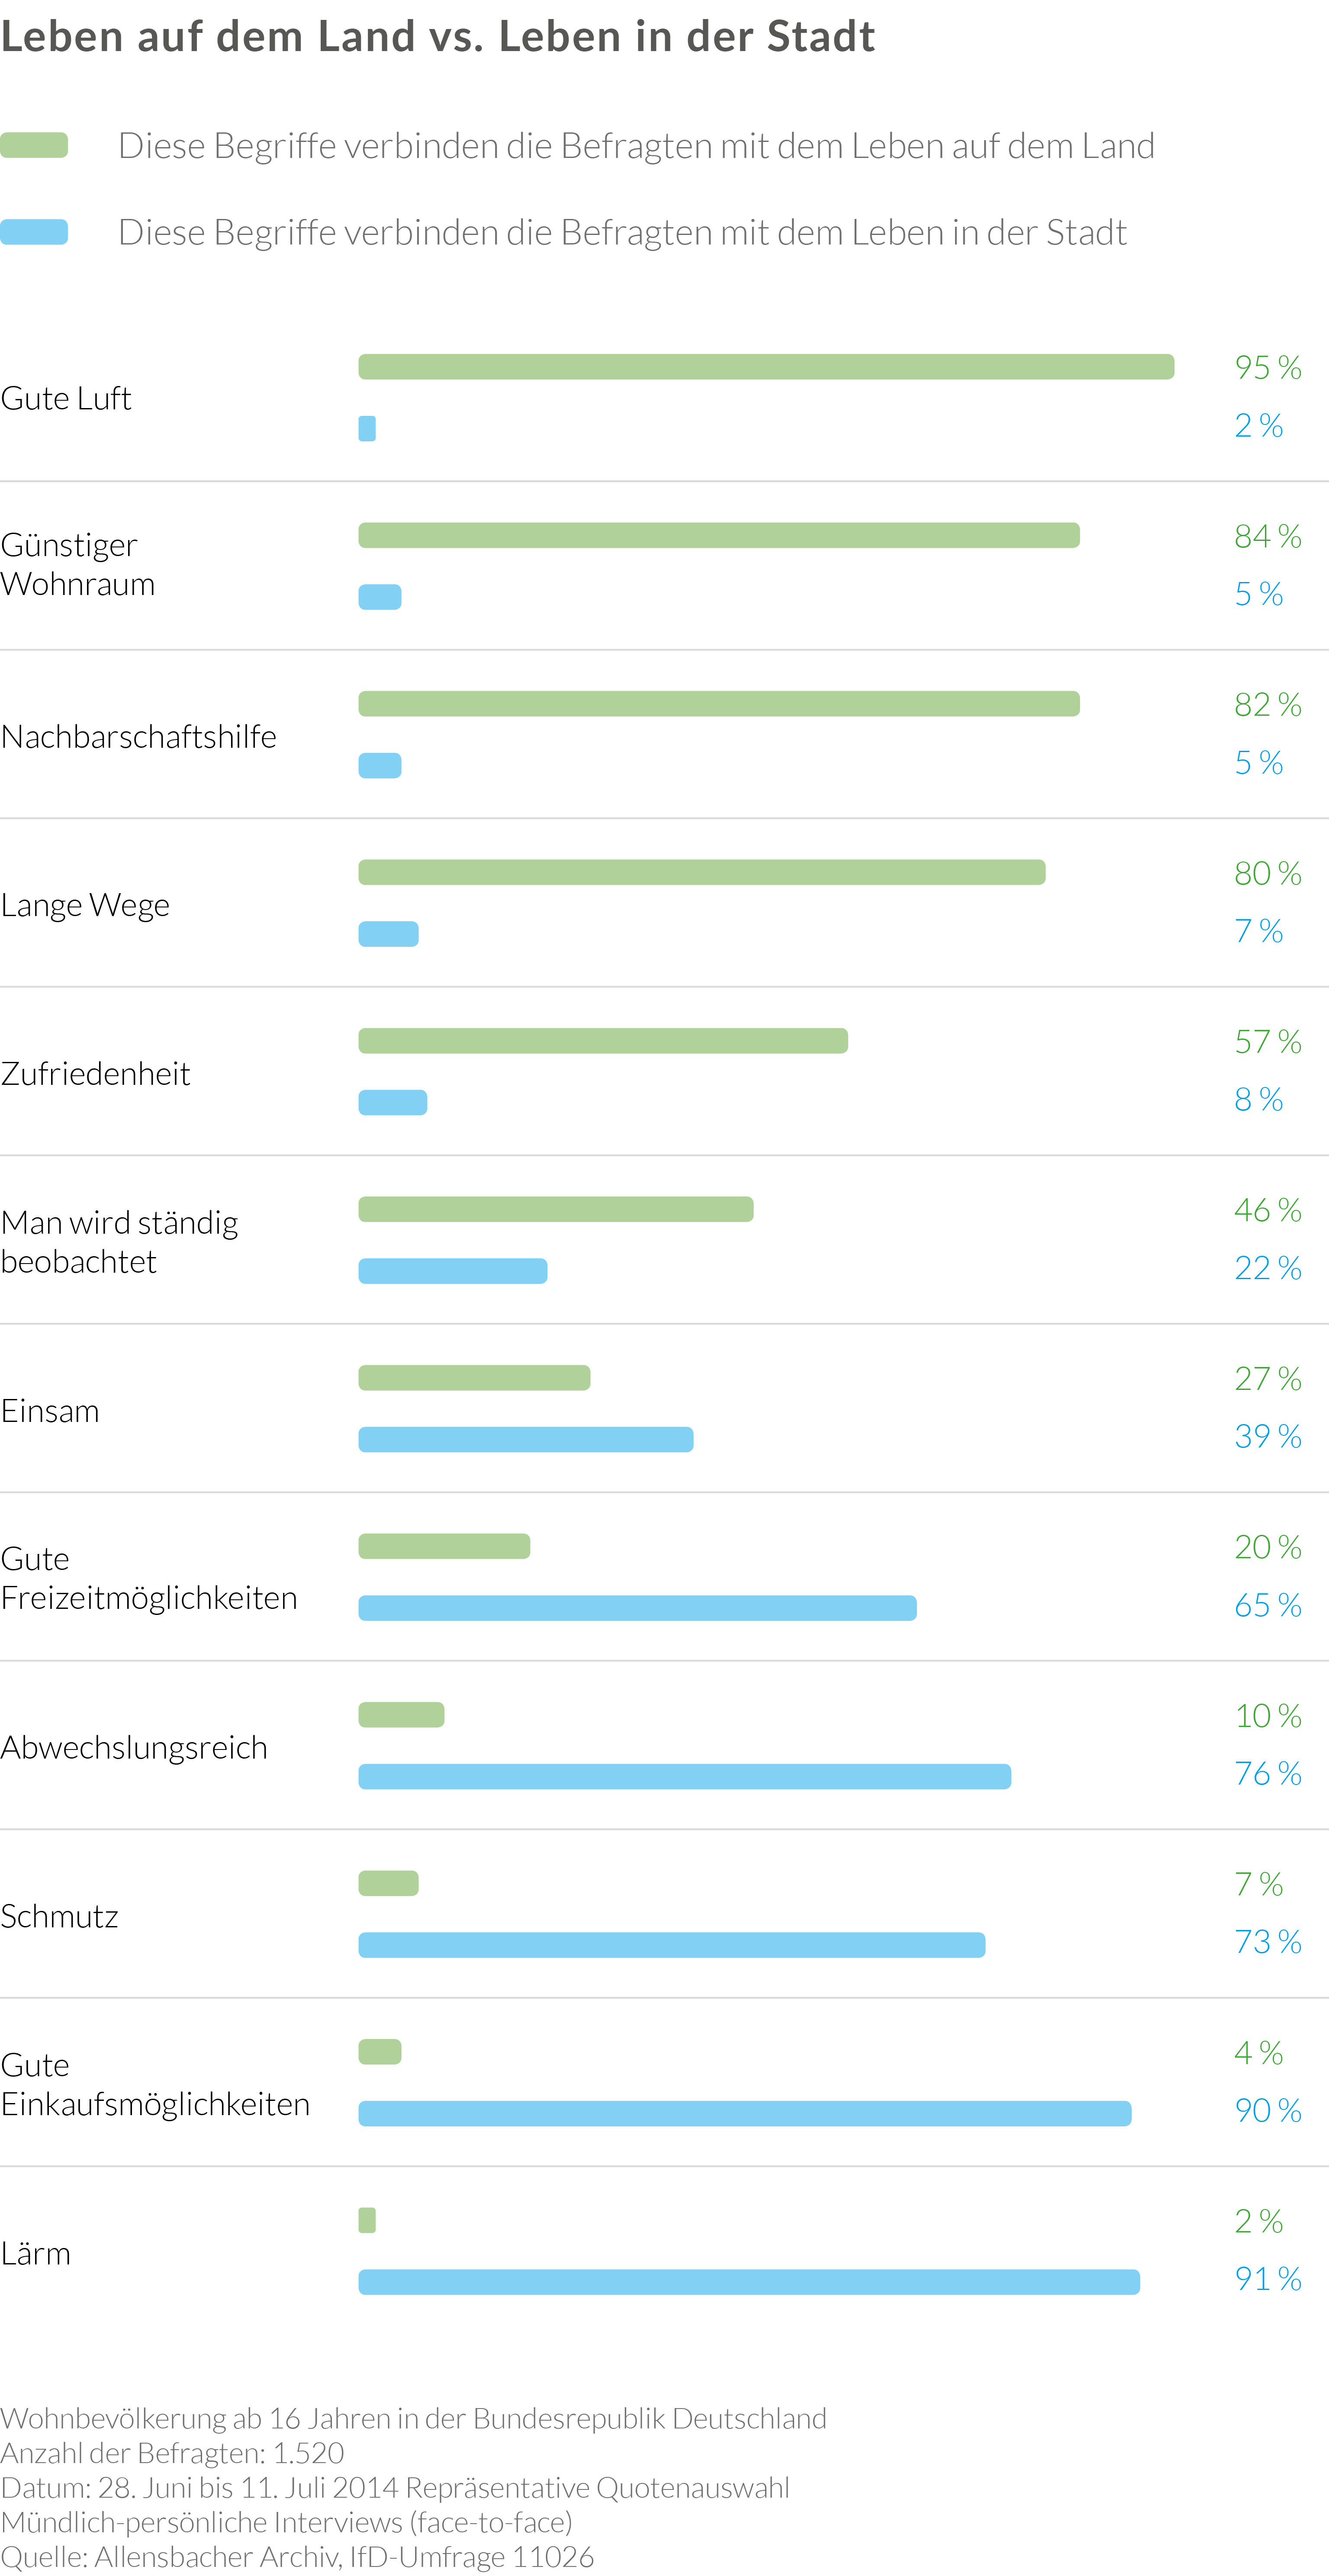
\includegraphics[width=11cm]{image_folder/SchaubildStadtVsLand_Umfrage.png}
\caption{Eigene Zeichnung, entstanden aus dem Vorbild von Dr. Thomas Petersen, Die Sehnsucht der Stadtbewohner nach Ländlichkeit S.13, Abb.3}
\label{fig:SchaubildStadtVsLandUmfrage}
\end{figure}

\begin{displayquote}
"Je mehr Menschen in der Stadt leben, je weniger Kontakt sie zum tatsächlichen Landleben haben, desto mehr wird das Land zu einer Projektionsfläche ihrer Phantasien."\footcite[S. 8]{Dr.ThomasPetersen2014DieLandlichkeit}
\end{displayquote}

Die Kategorien Stadt und Land können die räumliche, soziale und wirtschaftliche Realität nach dem Stadtforscher Angelus Eisinger kaum mehr beschreiben. Er schlät staddessen den Begriff „Stadtland“ als schwer trennbare, ineinanderfließende Siedlung vor und betont, dass es sich bei „Land“ lediglich um eine Idealisierung von Vergangenem handele. \footcite[Vgl.][S. 40]{Egnolff2015DieIdeal}

Laut Agraringenieur und Geschäftsführer des AgrarBündnis e.V Dr. Frieder Thomas hätten Landwirtschaftsvertreter des AgrarBündnis einerseits Verständniss für die aus seiner Sicht unrealistischen Vorstellungen des Landlebens, könnten sie aber trotz bester Absichten nicht erfüllen. \footcite[Vgl.][S. 27]{Thomas2015BauerlichkeitBegriff}

\begin{displayquote}
„Die Wünsche und Bilder, die hinter diesen Trends stehen, haben mit der Realität der Landwirtschaft und dem Leben auf dem Lande oft wenig gemein. In diesem Punkt sind sich die Verfechter bäuerlicher Landwirtschaft und die Strategen der Wachstumslandwirtschaft ausnahmsweise einig. Beide leiden auf ihre Art unter den vielfältigen Hoffungen, die auf den Bauern und dem Landleben ruhen. Beide stehen mitten zwischen den Bildern der Bauernhofidylle und dem Wachstumsdruck.“ \footcite[S. 27]{Thomas2015BauerlichkeitBegriff}
\end{displayquote}

Andere Vertreter würden wiederum eine Doppelstrategie verfolgen, in der sie einerseits die unrealistischen Visionen als ideologisch und unwissenschaftlich bezeichnen andererseits aber das realitätsferne Bild der Landwirtschaft mit einem Image der Idylle innerhalb von Werbestrategien untermauern.

Trotz der großen Distanz zur Realität bietet diese Sehnsucht nach einem besseren Leben auf dem Lande die Chance, die Art und Weise, wie wir Landwirtschaft betreiben und Lebensmittel handeln und behandeln, wieder zu einem zentralen Thema unserer Gesellschaft zu machen.

Festzuhalten wäre, dass trotz der unterschiedlichen Ansichten von städtischer und landwirtschaftlicher Bevölkerung die im Hinblick auf das Leben in ländlichen Gebieten bestehen, die Sehnsucht nach dem Leben auf dem Land genutzt werden kann. So werden Stadtbewohner immer sensibler wenn es um das Thema „Leben auf dem Land“ und Nahrungsmittel geht. So ist anzunehmen dass das Interesse für diese Thematik steigt und es zu einem zentralen Thema unserer Gesellschaft werden kann. Für die erfolgreiche Etablierung von UL gilt es jedoch im umkerhschluss eine übertriebene Erwartungshaltung gegenüber des ländlichen oder der ruralen Landwirtschaft durch innovative UL-Konzepte teilweise oder ganz zu befriedigen oder durch neue Ansätze zu ersetzen. So könnte UL auch zum Wohlbefinden der Stadtbevölkerung beitragen.

Die derzeite Situation der voranschreitenden Urbanisierung in Deutschland machen es zu einem repräsentativen Beispiel. Dennoch bleibt es zu Erforschen ob die „Landlust“ im Zuge der Verstädterung anderer Länder unter anderen kulturellen und soziologischen Hintergründen ähnlich stark ausgeprägt oder mit ähnlichen Ursachen verknüpft ist.

\section{Vergangenheit der Urbanen Landwirtschaft***}

Betrachtet man die Entwicklung und die bisherige Ausgestaltung von Städten, (wie im Kapitel 6 beschrieben) kann man dahinter leicht ein bestimmtes System entdecken. Neben der eher geplanten Verortung der Städte fand eine klare Differenzierung zum ländlichen Raum statt. Städte oder Siedlungen wurden zwar wie bereits erwähnt in Gebieten gegründet, die Versorgung durch Nahrung sicherstellten, dennoch führte die urbane Verdichtung dazu dass Nahrungsmittel, immer häufiger aus dem Umland in die Städte befördert werden mussten. Hierbei stellt die Megametropole New York ein Beispiel dar. Die Entwicklung der Stadt zeigt durch ihre verdichtete urbane Struktur eindeutig eine Tendenz, die keine rurale Landwirtschaft zulässt.\footcite[Vgl.][S. 146]{} Die Stadt selbst fungiert hierbei als Lebensraum und infrastrukturelle Anlaufstelle nicht als Raum für die Landwirtschaft. Diese Form des Städtebaus überdauerte und existiert bereits bis in die Gegenwart.

\subsection{Frühe Pläne zur Urbanen Landwirtschaft***}
Dabei existieren bereits seit mehr als 100 Jahren Stadtpläne durch ambitionierte Stadtplaner die das „Ländliche” als solches für das Leben in einer Stadt als essentiellen Bestandteil ansehen. Als Beispiel lässt sich die Vision des britischen Stadtplaners Ebenezer Howard mit seinem Konzept der Gartenstadt betrachten. Dieses bildet noch heute ein Vorbild für moderne Stadtplaner. In seinem Buch „Garden Cities of Tomorrow” welches bereits 1898 verfasst wurde vertritt er das Konzept eines Zusammenspiels von ruraler Landwirtschaft und urbanen Gebieten. Er betont zudem dass es sich bei den Gärten nicht nur um angelegte Ziergärten und Erholungsorte sowie Freizeitparks handelt sondern auch um "Freiräume", die Platz für den Anbau von Nutzpflanzen und die Aufzucht von Nutztieren bieten sollen. Neben den frühen Gedanken an eine Landwirtschaft innerhalb städtischer Strukturen ist der Aspekt der Versorgung und Infrastruktur ebenfalls betrachtet worden.

\begin{figure}[htbp]
\centering
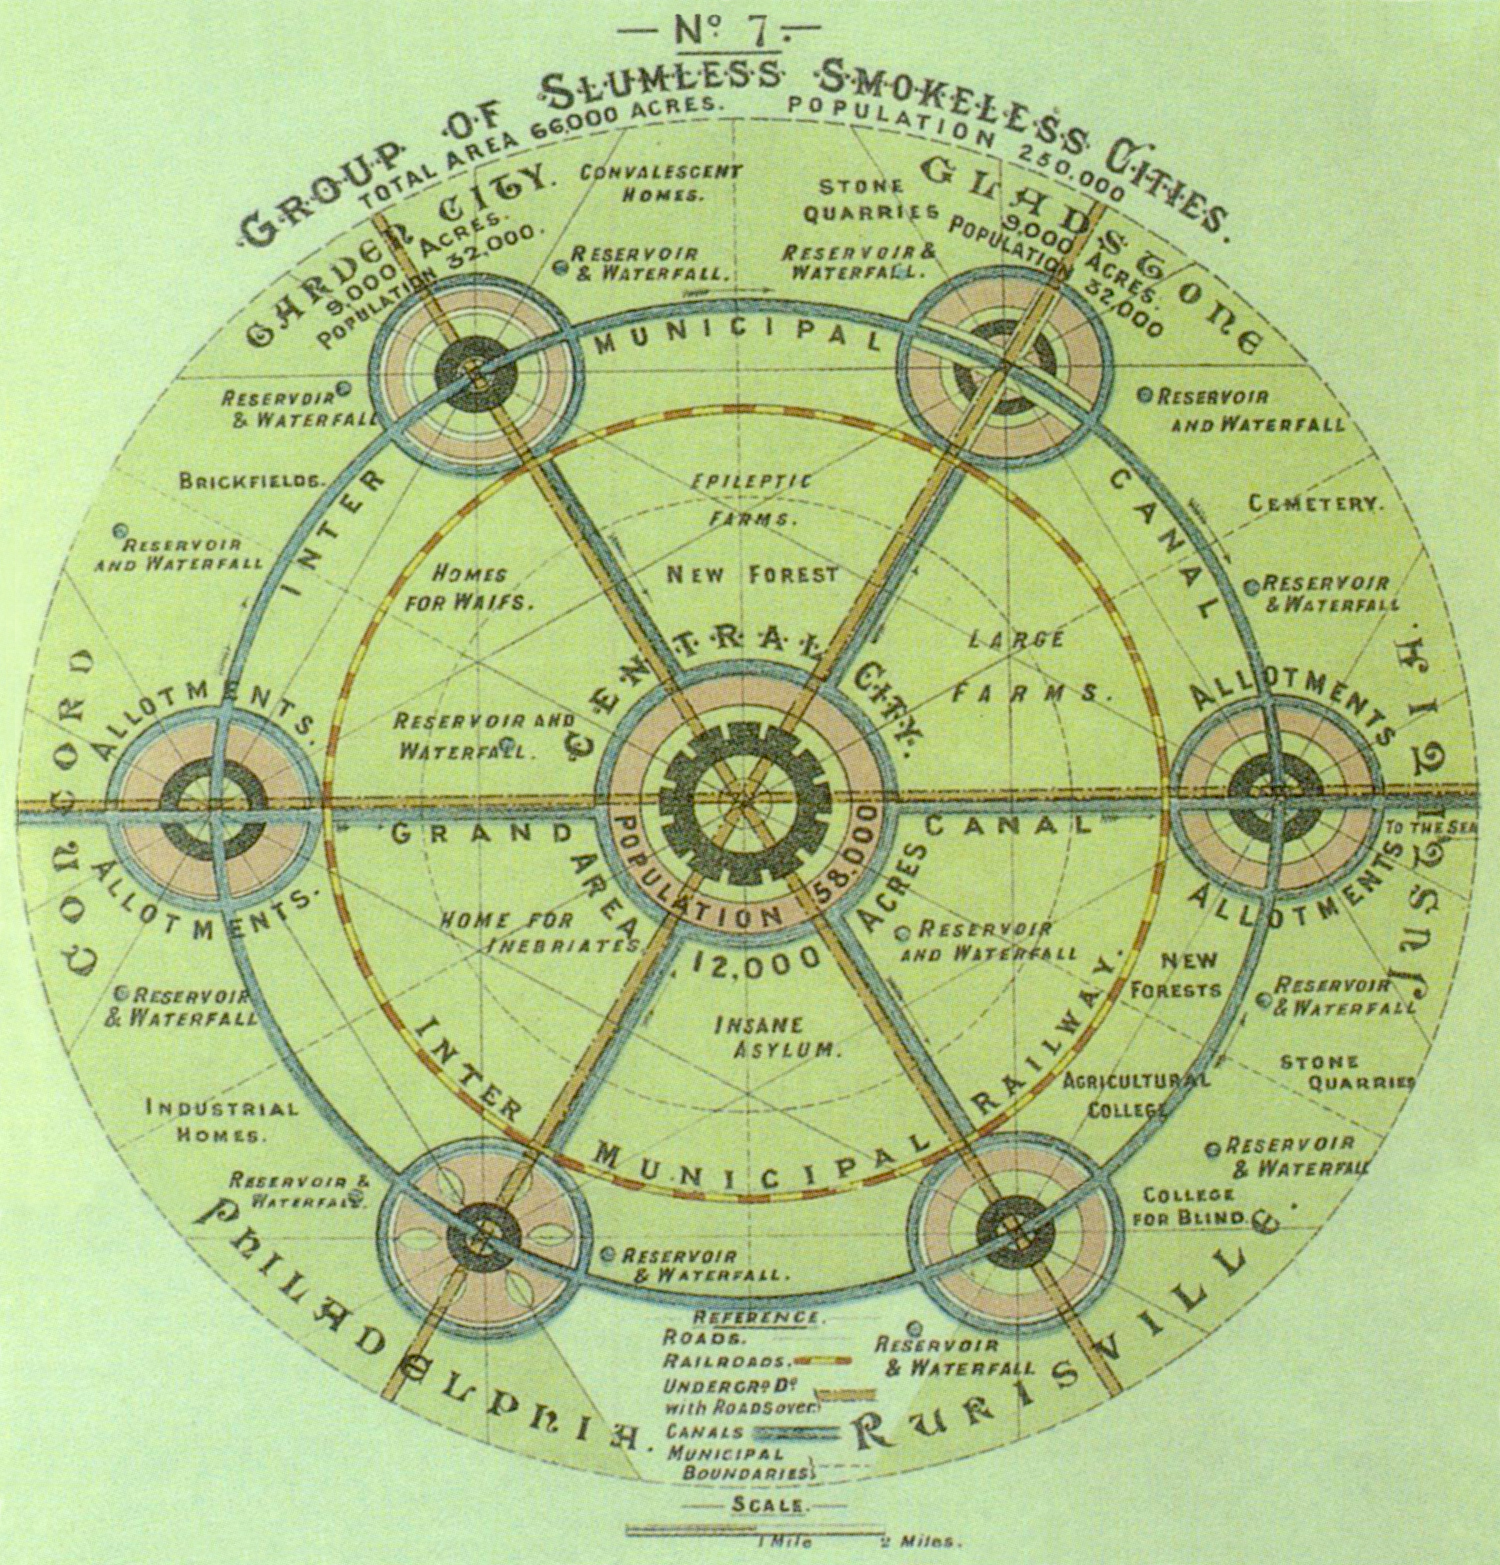
\includegraphics[width=10cm]{image_folder/GardenCityConcept_EbenezerHoward.jpg}
\caption{Konzept der Gartenstadt von Ebenezer Howard}
\label{fig:GardenCityConcept_EbenezerHoward}
\end{figure}

Interessant sind hier die „landwirtschaftlichen Gürtel” (ringförmige Anbauflächen um die Städte) und das Marktzentrum - den sogenanten "Crystal Palace" im Stadtzentrum. Dies ist ein ringförmiger Markt, der einem gläsernen Gewächshaus ähneln soll, das Waren aus der umliegenden Landwirtschaft direkt an den Verbraucher vertreiben sollte. Generell bleibt festzuhalten, dass Howard bereits 1898 nicht nur ein Konzept zur Verankerung von Landwirtschaft innerhalb von urbanen Gebieten erdachte sondern auch Ideen entwickelte, wie die urbane Bevölkerung mit den Lebensmitteln versorgt werden konnte.

Betrachtet man zum Beispiel Städte wie Boston, USA fällt auf, dass Grünflächen und Grünzüge nach dem Vorbild Howard's zwar eine wichtige Rolle in der Stadtplanung spielten, diese Grünflächen aber meist als Parks und Freizeitanlagen angelegt wurden. Dies war lange das von der Allgemeinheit verstandene Bild von Natur innerhalb einer Stadt.

Der urban landwirtschaftliche Aspekt wurde im 20. Jahrhundert durch nachfolgende Stadtplaner oft übergangen. Für den folgenden Stadtwachstum verkam die Urbane Landwirtschaft zur Ausgestaltung von mühevoll angelegten und vermeintlich natürlichen Ziergärten, die Grünflächen und Erholungsgebiete in die Städte bringen sollten. So bleibt die Frage, wie es zu dieser gegensätzlichen Entwicklung kam.

\subsection{Auszug der urbanen Landwirtschaft am Beispiel Deutschland***}
In Deutschland zeigt die Sozialgeschichte das im Jahr 1800 Großteile der Bevölkerung auf dem Land leben und aus der sogenannten Agrar-Gesellschaft bestehen. Zu diesem Zeitpunkt gab es in Deutschland lediglich drei Großstädte. 1835 Endstand dann allmählich das Eisenbahnnetz welches maßgeblich zur Ausbreitung der Industrialisierung beitrug. Durch das Eisenbahnnetz konnten Arbeiter zu Ihren Arbeitsstätten pendeln, welche sich wiederum durch das wachsende Netz stärker ausbreiten konnten. Zudem konnten Güter verstärkt kostengünstig transportiert werden. Dies führte in den folgenden Jahren zum Wachstum der Städte und Gemeinden und trug zudem zum Bevölkerungswachstum bei. 1850 bildete sich die industrielle Gesellschaft heraus. Zu diesem Zeitpunkt umfasste Deutschland bereits 35 Millionen Einwohner und zählte damit als eines der größten Länder Europas. Das enorme Städtewachstum wiederum lässt sich auf die Binnenwanderungen, den Wachstum der Bevölkerung, Gebietserweiterungen und Eingemeindungen zurückführen. 1900 besaß Deutschland bereits 33 Städte mit mehr als 100 Tsd. Einwohnern. Der Ausbau des Schienennetzes ist dabei nicht der einzige Faktor oder gar der Grund der Industrialierung oder des Bevölkerungswachstums, dennoch trug es massiv zur Ausbreitung der Bevölkerung bei. Heinrich Heine, einer der bedeutendsten deutschen Schriftsteller schrieb zu dieser Zeit:

„Welche Veränderungen müssen jetzt eintreten in unserer Anschauungsweise und in unsern Vorstellungen! Sogar die Elementarbegriffe von Zeit und Raum sind schwankend geworden. Durch die Eisenbahnen wird der Raum getötet, und es bleibt nur noch die Zeit übrig“. Dabei bot die Eisenbahn natürlich nicht nur Vorteile. Sie trug maßgeblich zur Veränderung des Landschaftsbildes bei und brachte Rus und Lärm in die Landschaften und Städte. Durch wachsende Infrastrukturen und der Industrie verdichteten sich im laufe der 20. Jahrhunderts die urbanen Gebiete massiv.

Lieberecht Migge schrieb 1926 in Hinblick auf diese Entwicklung "Das grüne Manifest" in dem er das "Leiden" der Städte zum Teil auf die Industrialisierung zurück führt. Er bezeichnet das "Land" (hier der ländlich rurale Freiraum) als Frischluftbehälter und als universale Erweiterungszone. Interessant ist hier auch dass er das "Land" nicht nur als physischen Freiraum sondern auch als Freiraum für den Geist des Menschen betrachtet in dem er seine Identität frei entfalten und entwickeln kann. Leitsätze wie "Schafft Stadtland" oder "Die Städte sollten Ihr eigenes Land umarmen" implizieren die Grundidee des ruralen Raumes innerhalb der Stadtgebiete. "Man Pflanze!" heißt es weiter. Aber das Gepflanzte soll auch Mehrwert erfüllen, keine einfachen nach Blumenbeet anmutenden Grünflächen um der Optik willen, sondern Parkanlagen, Spielplätze und Bäder, die der Allgemeinheit einen Mehrwert bieten. Aber auch Gedanken zur Selbstversorgung kommen auf. So schreibt er Beispielsweise von Nutzgärten mit einer größe von 80qm pro Einwohner auf denen Nahrungsmittel für den Eigenbedarf angebaut werden sollten. Was sich zunächst nach einer Wunschvorstellung anhört, könnte in Ausnahmesituationen Leben retten. Nach dem zweiten Weltkrieg litten beispielsweise viele Stadtbewohner an Nahrungsmangel. In der Nachkriegszeit änderte sich daher der Blick auf Urbane Landwirtschaft massiv. In städtischen Hinterhöfen wurden zum Beispiel auch Kartoffeln und Rüben angebaut. Erholungsparks und Spielplätze wurden in Nutzgärten gewandelt da reine Grünplätze mehr und mehr als unwirtschaftlich betrachtet wurden. Migge war sich dessen bewusst und versuchte in seinem Manifesto eine Art Richtlinie für den Städtebau zu entwickelten. So verurteilt er auch den Wohnraum einzelner Menschen über deren Bedarf hinweg und fordert ein verstärtkes Bewusstsein für Müll und Nahrungsmittelverschwendung. Die Städter sollten in einer Art Gleichgewicht mit dem Land leben. Dies betont er wei folgt: "Die Stadt muss auch geben dem Land - will sie leben vom Land". Eine der wichtigsten Architektonischen Eigenschaften von Städten, das Bauen von Wohneinheiten übereinander, verurteilt er und bezeichnet das "übereinander" als die "Wurzel allen übels". Dies ist zwar eine äußerst radikale Ansicht, repräsentiert aber den Wunsch nach freier Entfaltung und individualität. Er wünschte sich weiter ein neues Dasein im ländlich urbanen Raum welches durch harte Arbeit, Bescheidenheit und Naturverbundenheit geprägt sein sollte.

\subsection{Urbane Landwirtschaft aus globaler Perspektive (nicht ganz fertig ***)}

Betrachtet man UL aus globaler Perspektive, so kann man ihre lange Tradition innerhalb von gesellschaftlichen und kulturellen Praktiken in Bezug auf Stadt und Gemeinschaft erkennen. Die Anfänge der Ul reichen Jahrzehnte oder Jahrhunderte zurück bis sie schließlich in ihre jetzige Form mündet. Beispiele hierfür wären unter Anderem die europäischen Schrebergärten, Gemüsefelder in afrikanischen Kolonialstädten mit Wurzeln in alten kommunalen Praktiken, das chinesische System der Weiderverwendung des Nachtbodens oder die Chinampas von Mexiko-Stadt welche ein Anbausystem vor der Ankunft von Kolumbus darstellten.

Jac Smit, Joe Nasr und Annu Ratt beschreiben in Ihrem Beitrag \textbf{Urban Agriculture Yesterday and Today} zum Werk \textbf{Urban Agriculture: Food Jobs and Sustainable Cities} von 2001 die Anfänge der Urbanen Landwirtschaft. Dort lassen sich auch einige Beispiele für globale UL finden, welche vom Urban Agriculture Network aus verschiedenen Quellen Zusammengetragen wurden. Stand 2001.

\begin{displayquote}
\textbf{Afrika:}
\begin{itemize}
    \item Mali: Bamako ist mit Gartenbauprodukten autark und einige Produkte werden außerhalb der Metropolregion zum Verzehr versandt
    \item Uganda: In Kampala werden 70 Prozent des Geflügelbedarfs (Fleisch und Eier) innerhalb der Stadt produziert.
    \item Sambia: In Lusaka macht die Nahrungsmittelproduktion 33 Prozent des Gesamtverbrauchs der Hausbesetzer aus.
\end{itemize}
\textbf{Asien}
\begin{itemize}
    \item China: In den 1980er Jahren wurden über 90 Prozent des Gemüsebedarfs und über die Hälfte des Fleisch- und Geflügelbedarfs in den 18 größten Städten Chinas durch Produkte aus städtischen Provinzen gedeckt.
    \item Indonesia: In Jakarta werden fast 20 Prozent der von Hausbesetzern verzehrten Lebensmittel selbst produziert.
    \item Nepal: In Kathmandu deckten 37 Prozent der befragten Lebensmittelhersteller ihren Bedarf an pflanzlicher Haushaltsnahrung und 11 Prozent den Bedarf an Tiernahrung.
    \item Singapur: Achtzig Prozent des Geflügels und 25 Prozent des verzehrten Gemüses werden in der Stadt produziert.
\end{itemize}
\textbf{Europa}
\begin{itemize}
    \item Rumänien: Mit neuen Regierungsrichtlinien und -programmen von 1992 bis 1998 stieg die städtische Produktion von 14 auf 26 Prozent der gesamten landwirtschaftlichen Produktion.
\end{itemize}
\textbf{Amerika}
\begin{itemize}
    \item Kuba: Von 1992 bis 2000 stieg die städtische Nahrungsmittelproduktion um 300 Prozent und die Kinder essen viermal so viel Gemüse wie vor einem Jahrzehnt.
    \item USA: Dreißig Prozent der landwirtschaftlichen Produkte des Landes werden in Ballungsräumen produziert.
\end{itemize}
\end{displayquote}

Die Anforderungen an die Produktion von Nahrungsmitteln in der Stadt sind hoch. Pflanzen und Tiere müssen strapazierfähig gegenüber den städtischen Bedingungen sein und die begrenzte und kostbare Bodenfläche erfordert den Anbau von lukrativen und hochwertigen Produkten.\\ 
\\
Im Laufe der Zeit entwickelten einige Gesellschaften Techniken und Systeme, die die Landwirtschaft als Tätigkeit in die Stadt integrierten. Andere wiederum entwickelten die Städte getrennt von der Landwirtschaft. Dieser unterschiedliche Ansatz spiegelt auch unterschiedliche Einstellungen zur Art wieder, wie natürliche und menschengemachte Umgebungen miteinander umgehen und hat kulturelle Wurzeln.\\
\\
Im späten 19. Jahrhundert begannen Maschinen die landwirtschaftliche Arbeit zu erleichtern und die Produktion sowie die Vermarktung der Erzeugnisse stieg an. Die UL reagierte wiederum auf diese Entwicklung und spezialisierte sich beispielsweise auf Nischenmärkte, den Tauschhandel und den Devisenhandel sowie die Abfallverwertung. Die Informationsrevolution verbreitete dann das Wissen der städtischen Lebensmittelproduktion über nationale und kulturelle Grenzen hinweg und ermöglichte auch neue Formen des Marketings. Nach dem zweiten Weltkrieg schritt die Urbanisierung in manchen Ländern schneller voran als der Bevölkerungswachstum, die Wirtschaft oder Infrastrukturen. Daher fiel die Last der Lebensmittelversorgung mancherorts auf die Stadtbewohner selbst. Auf allen Kontinenten aber führte die Not an Bebauungsflächen oder Nahrungsmitteln zu intensivierter UL und zu einem erhöhten Bewusstsein für Landwirtschaft in Hinblick auf die Ernährungssicherheit. Ob UL nun von den ersten städtischen Siedlern entwickelt wurde um die Ernährung zu sichern oder ob sie durch die Schrittweise Veränderung der Nahrungsmittelproduktion entstand, eine Rolle spielte UL zu jeder Zeit. Teilweise war diese sogar unerlässlich.  \footcite[Vgl.][S. 1-4]{Smit2001UrbanCities}

\subsection{Beispiele aus der Geschichte der urbanen Landwirtschaft}


Laut Smit, Nasr und Ratt gäbe es sichere Hinweise auf groß angelegteBaumkulturen in Mayastädten. Hinweise lassen sich in Städten wie Caracol Lamanai und Belize finden. Die bevölkerungsdichte in Caracol betrug demnach ca. 1.000 Menschen pro Quadratkilometer bei einer Gesamtbevölkerung von 115.000 - 150.000 Menschen.\footcite[Vgl.][S. 5-6]{Smit2001UrbanCities}Zum Vergleich: Das \textbf{Amt für Statistik Berlin-Brandenburg} gibt an, dass am 31.12.2017 in Berlin ca. 4.055 Menschen pro Quadratkilometer in der deutschen Hauptstadt lebten.\footcite[Vgl.]{AmtfurStatistikBerlin-Brandenburg2017NoTitle}Die Stadtlandschaft von Caracol bestand aus dichten Gebäudegruppen die mit landwirtschaftlichen Terassen durchzogen waren. Forscher glauben, dass diese Archtiektur seinen Fokus auf die Selbstversorgung setzte. Die Terassen und Stauseen durchzogen die gesamte Stadt.\footcite[Vgl.][S. 5-6]{Smit2001UrbanCities}

Landwirte reaktiverten mit Hilfe von Archiologen an mehreren Standorten in Peru, Guatemala und Mexiko dei alten Systeme der UL und erhielten interssante Erkenntnise über die damalige Landwirtschaft.\footcite[Vgl.][S. 6]{Smit2001UrbanCities}{zietiert nach Cardich und L. Fowler, 1987 National Geographic Research, Vol. 3, No.1.}
In einem Fall unterstützen die Produktionsniveaus zwei Familien auf 1 Hektar (0,40 Hektar). In einem zweiten Fall wäre eine Wiederbelebung der alten Terrassentechnik speziell erfolgreich. Eine der wichtigsten Erkenntnisse ist der Einsatz von Aqua-Terra-Systemen, in denen Wasser- und Landpflanzen in Symbiose produziert werden. Solche Systeme sind besonders relevant für die städtische Landwirtschaft, da sie in Gebieten mit weniger gutem Boden, steilen Hängen und Feuchtgebieten effektiv sind. 

\begin{figure}[htbp]
\centering
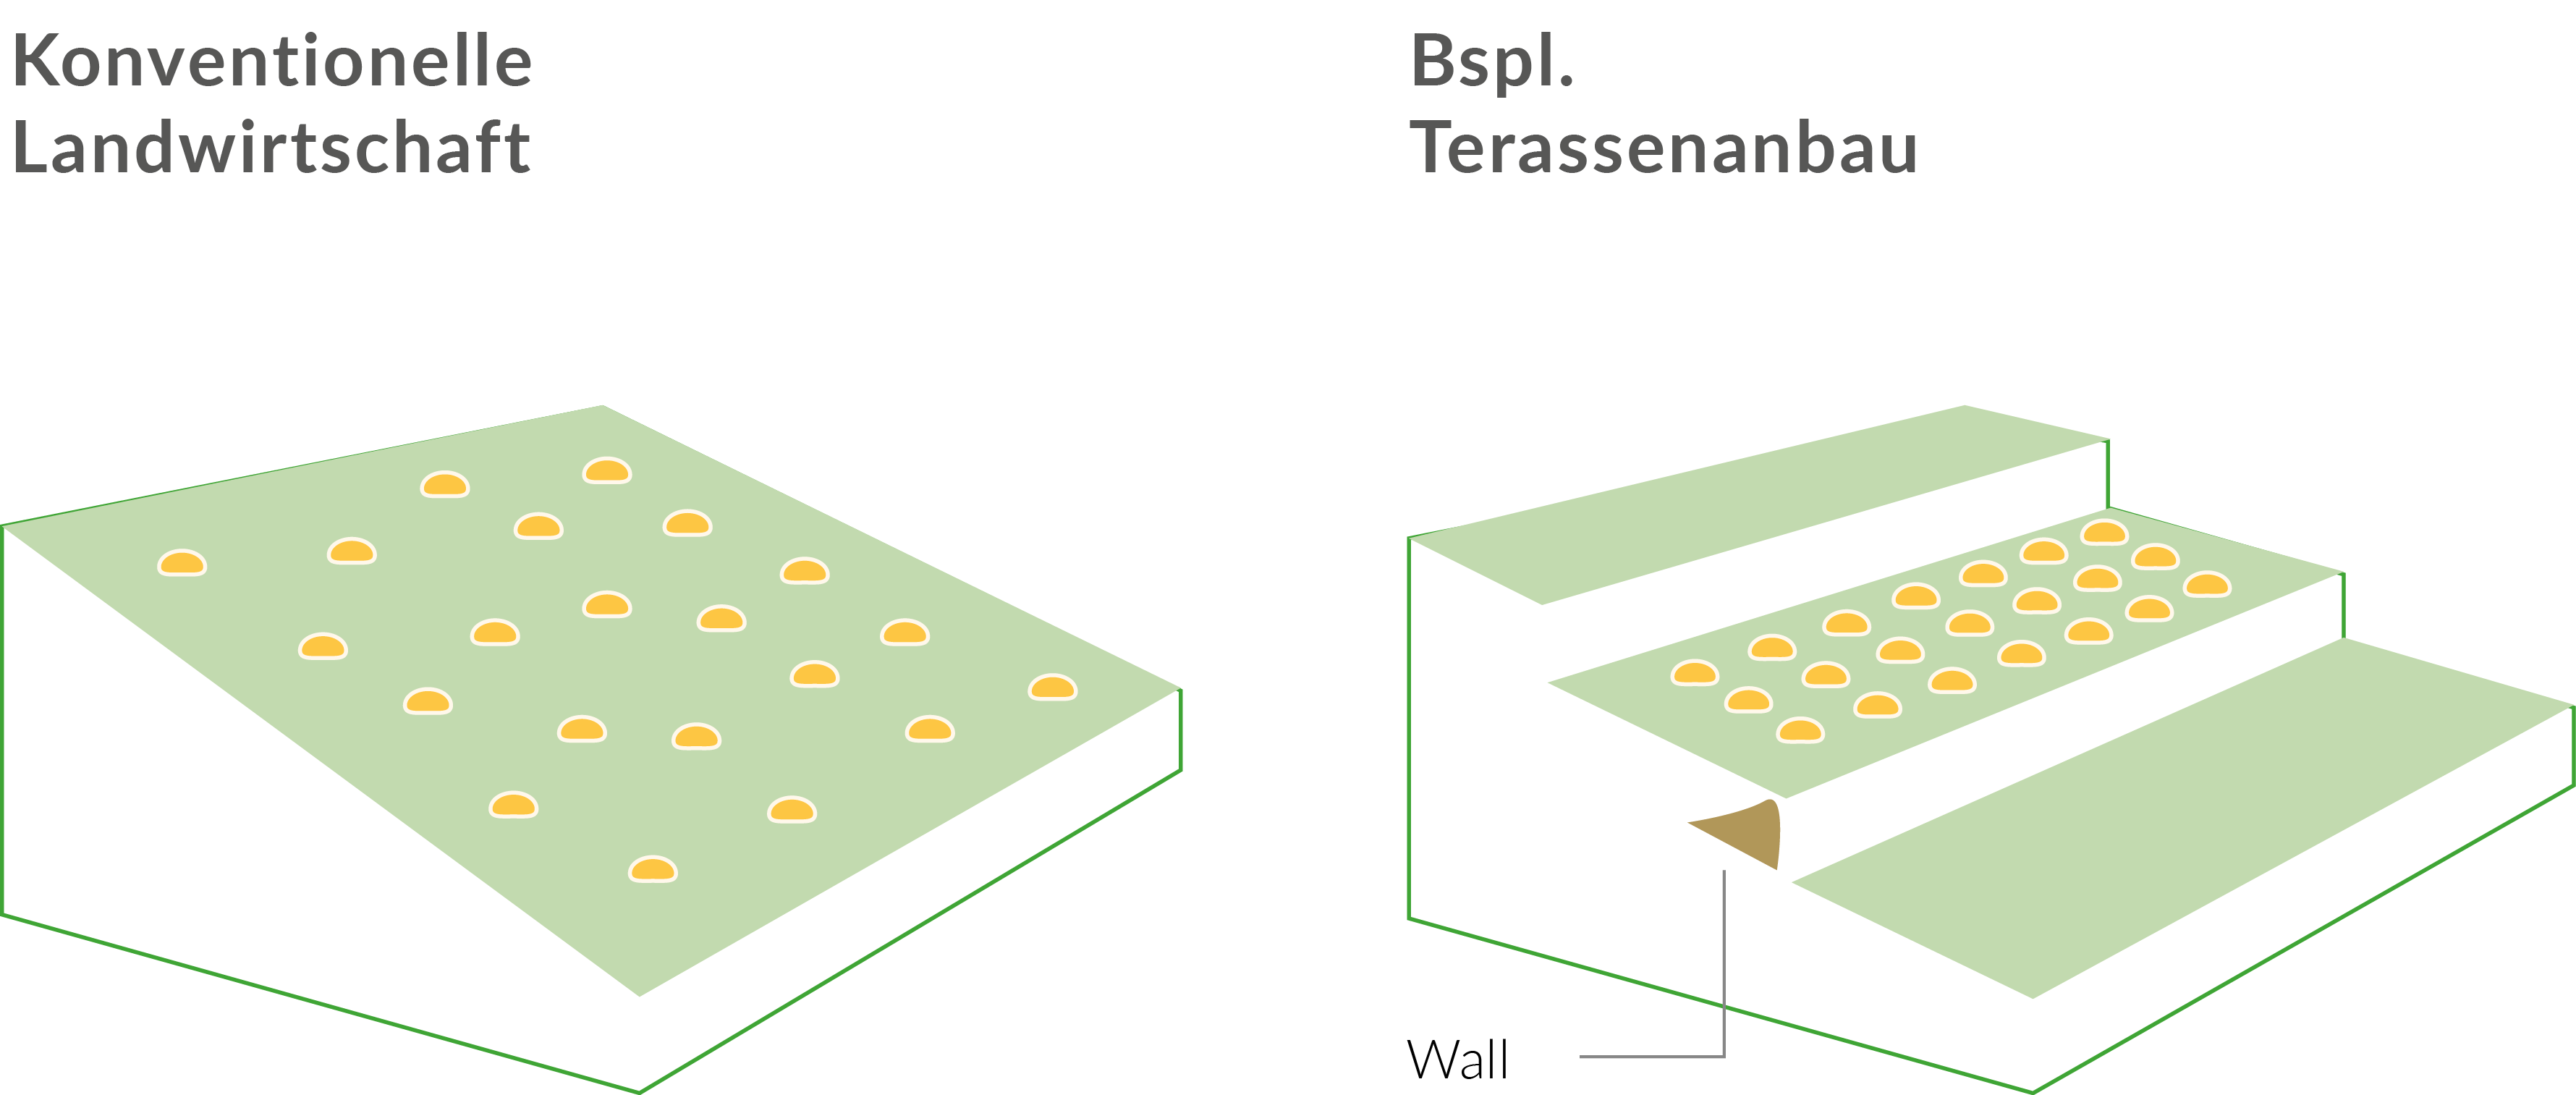
\includegraphics[width=10cm]{image_folder/SchaubildTerassenanbau.png}
\caption{Vereinfachtes Konzept des Terrassenanbaus, Eigene Zeichnung}
\label{fig:Terassenlandwirtschaft}
\end{figure}

In vielen alten Systemen würde zudem das Klima durch Techniken wie Bewässerung und Erwärmung des Bodens und der Luft gemildert, um die Vegetationszeiträume zu verlängern. In Europa würde beispielsweise Kompost, einschließlich Pferdemist, schon seit langem zur Beheizung von erhöhten Gemüsebeeten verwendet. Seit hunderten Jahren und in verschiedenen Teilen der Welt wären Anbau und Viehzucht innerhalb und außerhalb der Stadtmauern Standard. Bevor in der zweiten Hälfte des 19. Jahrhunderts "moderne" städtische Abwassersysteme entwickelt wurden, wäre die städtische Landwirtschaft die wichtigste Behandlungs- und Entsorgungsmethode für städtische Abfälle gewesen.\footcite[Vgl.][S. 6-7]{Smit2001UrbanCities}

Die Liste der Arten von urbaner Landwirtschaft in alten Kulturen ist lang und beschreibt die Wichtigkeit von marnknaher Landwirtschaft vor der Erfindung von Kühlsystemen oder schnellen Transportmitteln. Aber auch in späteren Jahren beweist die urbane Landwirtschaft ihre Relevanz.

Ernst May erdachte beispielsweise 1922/23 Trabantenstädte erdachte zu, die von "Kulturbändern" umgeben wurden, auf diesen dann eine intensive Landwirtschaft entstehen sollte. Gemüse und Kleinvieh von Kleinbauern sollte so herangezogen und gezüchtet werden, welches dann als Nahrungsmittel für die Siedlungen gefördert werden sollte. Dieser Ansatz floss teilweise in den 1920er Jahren in den Städtebau mit ein und stärkte dabei das Kleingartenwesen.

Mitte der 1970er Jahre erreichte dann die Idee der Community Gardens Europa. Hier nutzten fleißige Anwohner benachteiligter Viertel, beispielweise in New York, Brachflächen der Stadt und pflanzten Blumen, Gemüse und Kräuter an. Diese Bewegung erreichte Deutschland etwa 1990. Berlin gilt heute als eine der deutschen Hochburgen für Gemeinschaftsgärten.\\
\\
Zusammenfassend lässt sich sagen, dass urbane Landwirtschaft häufig als Versorgungsrettung betrachtet wird. Das Bewusstsein für die vermeintlich lebensrettende Methode der Landwirtschaft scheint immer dann stark zu wachsen wenn es den Bewohnern urbaner Gebiete besonders schlecht ergeht. Dies wurde auch 2007 deutlich als schwere Waldbrände in Griechenland wüteten. Die Krise führte zu einem vermehrten Anbau von Nahrungsmitteln innerhalb der griechischen Städte und führte sogar zur Ausbeutung von städtisch landwirtschaftlichen Räumen durch Zivilisten. Seit 2012 wird die urbane Landwirtschaft von der Zivilgesellschaft oder den einzelnen Gemeinden verbreitet.

Ein weiteres Beispiel für den Antrieb von Urbaner Landwirtschaft in Kriesenzeiten lieferte Kuba in den 90er Jahren. Durch den Zusammenbruch der Sowjetunion kam es auf der Insel auch zum Zusammenbruch der dortigen Wirtschaft, da diese stark von der sowjetischen Ölversorgung abhing. Durch den fehlenden Rohstoff konnten beispielsweise keine Erntemaschinen betankt werden. Zudem mangelte es auch an Düngern und Pestiziden. Die Einwohner der Insel setzten immer stärker auf die urbanen Anbaumethoden. Heute gehört der Inselstaat zu den Ländern die große Fortschritte zur Bekämpfung von Hunger durch Urbane Landwirtschaft gemacht haben.

Detroit welche von einer starken Wirtschaft profitierte geriet vor Jahrzehnten in eine schwere Krise. Die einstige florierende Automobilbranche liegt brach. Dadurch zogen viele arbeitslose Einwohner aus der Stadt. Durch die ungenutzten urbanen Gebiete konnte aber in den darauffolgenden Jahren eine aufsteigende Landwirtschaft entstehen. Brachland und Dachterrassen wurden nun zu ca. 1200 fruchtbare Gärten verwandelt. „Nach einer Studie der Michigan State University könnte Detroit mit Stadtfarmen, Nachbarschaftsgärten und Gewächshäusern drei Viertel ihres Gemüses und vierzig Prozent ihres Obstes selbst produzieren.“ https://www.bzfe.de/inhalt/gemuese-statt-cadillac-urban-gardening-in-detroit-27424.html


\section{Gegenwart der urbanen Landwirtschaft}
\subsection{Aufgaben und Motivation***}

Wie gut ein Land versorgt ist hängt von vielen Faktoren ab. Darunter zählt der wirtschaftliche Status, die Verfügbarkeit von Ressourcen, die jeweilige Ernährungspolitik und wie gut die Infrastruktur zur Lebensmittelversorgung (Transport, Lager, Vermarktung uvm.) ist. Demnach unterscheiden sich die Aufgaben, die urbaner Landwirtschaft zugewiesen werden je nach dem „Entwicklungsgrad“ des umgebenden Landes.\footcite{Smit2001UrbanToday} In Industrieländern ist sie von sozialpolitischer Natur.\footcites[][S. 21]{Berges2014UrbaneStadt}[S.26f]{Smit2001UrbanToday} In Entwicklungsländern hingegen dient sie vorwiegend zur Subsistenz oder als zusätzliches Einkommen für die Stadtbewohner. \footcites[Vgl.][S.75]{Nugent2000TheEconomies}[S.26f]{Smit2001UrbanToday}\\
\\
Warum urbaner Gartenbau noch bedeutend für Entwicklungsländer ist, erläutert Moustier: \footcites[Vgl.][S.6ff]{Moustier2007UrbanSupplier} Gängig sei der Anbau von schnell verderblichen Lebensmitteln wie Blattgemüse oder Tomaten. Durch die Nähe zur Stadt ist der Transportweg in der Regel kürzer und die Produkte gelangen zeitnah zum Konsumenten. Zusätzlich ist in den meisten Fällen die Lieferkette kürzer, was den Preis der Lebensmittel senkt. Bei weniger verderblichen Lebensmitteln schwanke der Anbau zwischen den Stadtrandgebieten und ruralem Anbau. Den Konsumenten sei auch die Frische der Produkte besonders wichtig, da ihnen oft eine geeignete Lagerung wie Kühlschränke fehle. Bedenklich sei allerdings die Qualität der Lebensmittel durch die verunreinigte Wasser- und Bodenqualität sowohl in der Stadt als auch im Umland. Jedoch sorge die Nähe für einen besseren Informationsaustausch zwischen Konsument und Produzent zum Anbau. Das erleichtert den städtischen Gemeinden und den Menschen vor Ort die Kontrolle ihrer Ernährungssicherheit. Darüber hinaus habe urbane Landwirtschaft oft damit zu tun, dass viele Städte geschichtlich an rohstoffreichen Gegenden angesiedelt waren und das Umland von Städten daher gute Anbaubedingungen vorweist. Die saisonalen Bedingungen spielen, Moustier zufolge, ebenfalls eine wichtige Rolle. In „schlechten“ Jahreszeiten sind Stadtbewohner angewiesen auf die Zufuhr von ferner angebauten Nahrungsmitteln. \\
\\
Auch der private Anbau in diesen Städten sei nicht zu vernachlässigen. Zu der Frage, warum Stadtbewohner in diesen Regionen UL betreiben, ergaben sich aus Nugents Umfrage im Jahr 2000 mehrere Antworten. \footcite[Vgl.][S.74]{Nugent2000TheEconomies} Zu den Hauptgründen zählte der Eigenverbrauch, die Einkommenssteigerung und ökonomische Krisen. Besonders die Unsicherheit der Ernährungslage sei eine häufige Sorge, die Stadtbewohner antreibe. Zum Beispiel in Accra (Ghana) sei Viehbestand eine sichere Anlage in schweren Zeiten. Auch die Höhe des Einkommens beeinflusse den Aufwand, den jene Haushalte für UL betreiben. Zezza et. al. zeigten durch ihre Datenerhebung wie aktuell\footnote{Diese Datenerhebung fand 2010, also zehn Jahre nach Nugents Untersuchungen statt. Der Grund, den Zezza et. al. für ihre Arbeit nannten, war der Mangel an repräsentativen Daten dieses Forschungsbereichs.} Nugents Punkte noch sind:
\begin{displayquote}
„With very few exceptions, a clear negative correlation between participation in agricultural activities and level of welfare is noted. Participation rates for the poorest quintile are extremely high, over 50\% in 8 out of 15 countries, proving how urban agriculture plays an important role for a non-negligible number of poor households in the developing world.“\footcite[S.268]{Zezza2010UrbanCountries}
\end{displayquote}

Diverse Organisationen setzen sich für den Einsatz von UL als Lösung für Unterernährung und Armut in Entwicklungsländer ein, eines der größten ist wohl die Ernährungs- und Landwirtschaftsorganisation der Vereinten Nationen (FAO - The Food and Agriculture Organisation of the United Nations).\footcite[Vgl.][S.6ff]{FAOAboutNations} In diesem Zusammenhang äußert sich FAO Generaldirektor Jaques Diouf:

\begin{displayquote}
„\lbrack...\rbrack urban poverty tends to be fuelled by people migrating towards the cities in an attempt to escape the deprivations associated with rural livelihoods. Partly due to the rural decline, the world is urbanizing at a fast pace and it will not be long before a greater part of developing country populations is living in large cities. Therefore, urban food security and its related problems should also be placed high on the agenda in the years to come.“\footcite[S.5f]{FoodandAgricultureOrganizationoftheUnitedNations2006The2006}
\end{displayquote}
In Industriestaaten sei die Unsicherheit über die Lebensmittelversorgung hingegen nicht so stark wie in Entwicklungsländern. Smit et. al. geben dafür drei Gründe an: Zum einen sei das Verhältnis zwischen den Lebensmittelkosten und dem urbanen Haushaltsbudget in Industrieländern geringer. Während Stadtbewohner im globalen Norden ein Drittel bis ein Fünftel ihres Haushaltsbudgets für Essen verbrauchen, liegt der Anteil der Lebensmittelkosten in ärmeren Ländern zwischen ein Drittel und vier Fünftel. Ein weiterer Grund sei, dass die Infrastruktur zur Nahrungsmittelversorgung vollständiger sei. Und der dritte Punkt sei die höhere Lebensmittelqualität aber auch, dass sie zugänglicher seien für die Stadtbevölkerung. \footcites[Vgl.][S.27]{Smit2001UrbanToday} Smit et. al. zufolge wachse das Interesse an urbanen Gemeinschaftsgärten in Europa und den vereinigten Staaten. Der Antrieb dafür sei unter anderem die Sorge um die Nahrungsmittelqualität der globalen Lebensmittelkonzerne. Angeknüpft dazu seien soziale politische Motive. Ferner führte das Leibniz-Zentrum für Agrarlandschaftsforschung 2011 bis 2014 eine Innovationsanalyse zu urbaner Landwirtschaft in den vereinigten Staaten und Deutschland aus. Eines der Erkenntnisse war, dass heutige UL-Formen in den untersuchten Ländern vorwiegend soziale Neuerungen zeigen \footcite{Berges2014UrbaneStadt}. Passend dazu ist die mediale Wahrnehmung des Begriffs Urban Gardening in Deutschland, den Egnolff vor drei Jahren untersuchte. Ihren Analysen zufolge werde dem Begriff zwar auch ökonomische Bedeutung zugewiesen, allerdings seien die politische, Lifestyle-, soziale als auch nachhaltige Bedeutung nicht zu vernachlässigen.\footcite[Vgl.][S.119ff]{Egnolff2015DieIdeal}. 
%------------------------
% über Motive von innovativen Konzepten schreiben: verdichtete Städte, Zuwachs...
%------------------------

\subsection{Aktuelle Beispiele urbaner Landwirtschaft}

%Die Urbane Landwirtschaft hat es mittlerweile immer öfter in die öffentlichen Medien geschafft. Durch die Ansätze des Guerilla Gardenings oder Skyfarmings erzeugt das Themenfeld auch größeres Interesse, beinhaltet aber auch Projekte und Ansätze ohne deutlichen Mehrwert. Dies bedeutet das manche Methoden der UL einen unzureichend Nachhaltigkeitsaspekt bieten oder schlichtweg nicht wirtschaftlich arbeiten. Beispiele für UL folgen. Es kommt hinzu, dass die UL keine nennenswerte Rolle in der Ausbildung von Landwirtschaftsberufen spielt. Das Bewusstsein für UL in der modernen Stadt ändert sich aber durch ambitionierte Architekten, Stadtplaner und Einwohner stetig und Brachflächen innerhalb von Städten werden nicht mehr nur einfach begrünt sondern nehmen auch einen immer größeren Platz in der professionellen Planung ein um einen Mehrwert solcher Flächen zu gewährleisten.

%"Man versucht die Landwirtschaft als Partner zu gewinnen, um die Freiflächen in der Stadtregion zu unterhalten und als öffentlichen Raum zu bespielen." Frank Lohrberg - Urban Gardening Christa Müller


Eine umfassende Statistik über die weltweite Verbreitung von UL mit all den dazugehörigen Arten gibt es derzeit nicht. Nur die geschätzte Statistik von Smit et. al. aus dem Jahr 2000 gibt - wenn auch nur im Bezug zur konventioneller Landwirtschaft - ein Gefühl für die Größenordnung heutiger urbaner Landwirtschaft.
\begin{figure}[htbp]
    \centering
    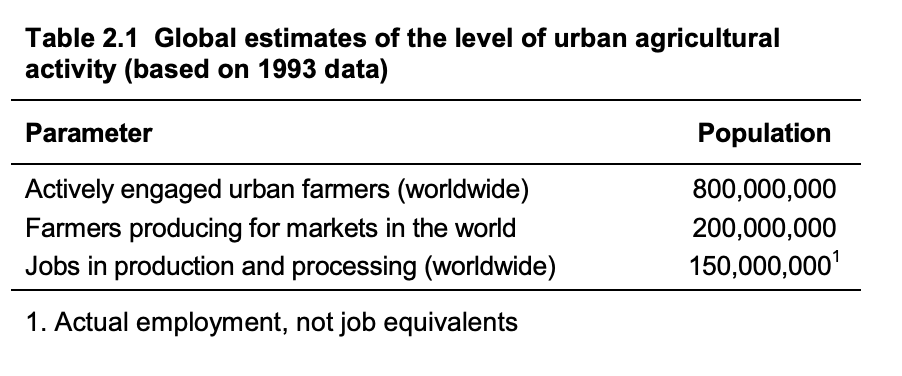
\includegraphics[width=10cm]{image_folder/800000ul.png}
  \caption{Schätzungen des Urban Agriculture Network basierend auf dem Erfahrungen und Beobachtungen von Jac Smit und auf dem Gebiet der Hochrechnungen aus Statistiken verschiedener amtlicher Volkszählungen und professionelle Umfragen. Die Absicht sei es, eine Miniaturansichtsskizze von der Bedeutung der Branche. Eine systematischere Schätzung würde eine einen wesentlichen Beitrag zum Wissensbestand leisten.}
  \label{fig:plantagon}
\end{figure} 

Unabhängig davon lässt sich sagen, dass die aktuellen Formen vom Gemüseanbau am Balkon bis hin zu innovativen Hochhauskonzepten reichen. \footcites[Vgl.][S.24]{Berges2014UrbaneStadt}[S.268]{Zezza2010UrbanCountries}[S.14]{Al-Kodmany2018TheCity} Wie in den Grundlagen beschrieben, teilt sich UL unter anderem in subsistenziell, soziokulturell und kommerziell motivierten Formen auf. In Anbetracht der zentralen Fragestellung dieser Forschungsarbeit stehen kommerzielle UL-Formen im Fokus der Untersuchung. Da diese Form im Vergleich zur soziokulturellen und subsistenziellen die größte Menge an Konsumenten erreicht, ist ihre Auswirkung groß genug, um sie auf Nachhaltigkeit zu prüfen. Daher widmet sich Kapitel 10 vorallem dieser Landwirtschaftsform. Dennoch ist es hilfreich einen Eindruck zur erhalten, wie unterschiedlich sich urbane Landwirtschaft durch ihre Motive ausdrückt. Das zeigen folgende Beispiele:

\begin{figure}[htbp]
    \centering
    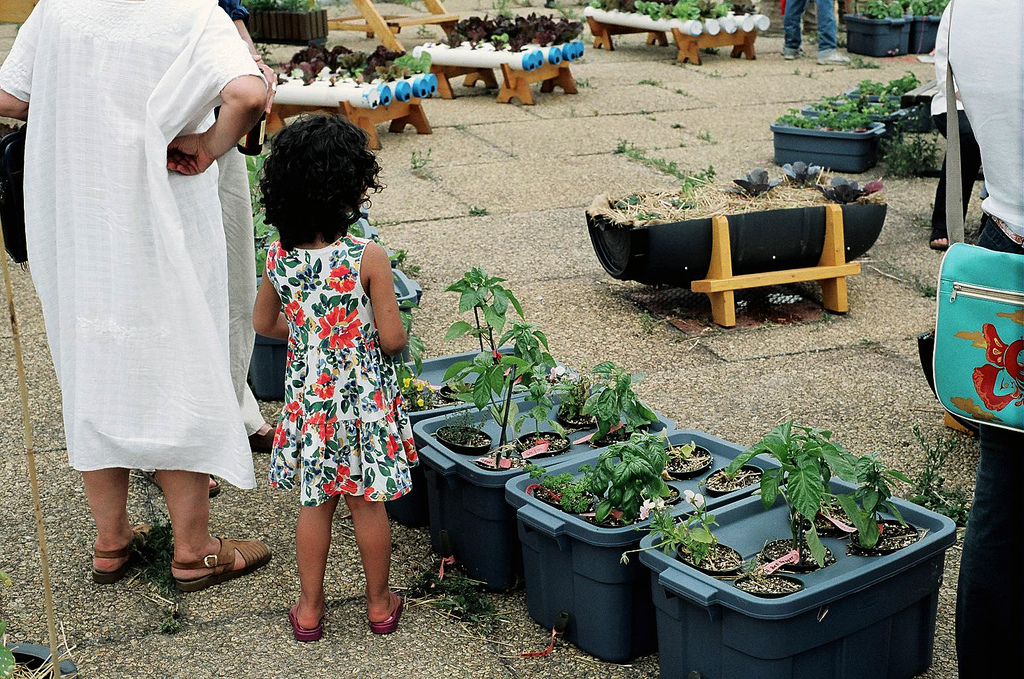
\includegraphics[width=14cm]{image_folder/simplified_hydroponics_jack_sanford.jpg}
  \caption{„Simplified Hydroponics“ von Jack Sanford}
  \label{fig:shydroponics}
\end{figure} 

\subsubsection*{Vereinfachte Hydrokultur in Ecuador}
Wie im vorigen Kapitel beschrieben, unterstützt die FAO urbane und peri-urbane Projekte gegen Hunger und Armut. Besonders seit 1991 fördere sie Workshops zum vereinfachten Hydrokulturanbau (Pflanzenanbau mit Substraten anstelle von Erde).\footcites[Vgl.][o.P. (S.1)]{Stajano2003SIMPLIFIEDEcuador} Die  Hydrokultur unterscheide sich von hochwertigen Variante in dem Sinne, dass sie - im Vergleich zu industriellen Produktionen - ausgelegt ist auf die Ernährung von gering verdienenden Familien und daher wenig Ressourcen verwendet. Vorteile dieser Methode seien unter anderem die einfache Erlernung, die Vermeidung von verseuchtem Boden und flexible Anbaustellen in Städten. Desweiteren können alte Behälter dafür wiederverwendet werden und der Anbau erfordere weitaus weniger Wasser als üblicher Feldanbau. Ein Beispiel dazu ist das im Jahr 2000 umgesetzte Hydrokulturprojekt in den urbanen Regionen Ecuadors.\footcite[Vgl.][o.P. (S.2f)]{Stajano2003SIMPLIFIEDEcuador}. Ziel des Projektes war es Kindern unter sechs Jahren Zugang zu qualitativen Lebensmitteln zu bieten und einkommensarmen Familien durch diese Seminare nicht nur diese Anbaumethode beizubringen sondern auch einen besseren Lebensstandard zu bieten und im Idealfall ein sicheres Einkommen zu ermöglichen. Schlussendlich wurden nicht nur die aufgelisteten Ziele erreicht, darüber hinaus wurden die betroffenen Kinder durch die gesunde Ernährung seltener krank. Das Projekt kam so gut bei den jeweiligen Gemeinden an, dass Interesse besteht den erlernten Anbau eigenständig auszubauen. 

\begin{figure}[htbp]
    \centering
    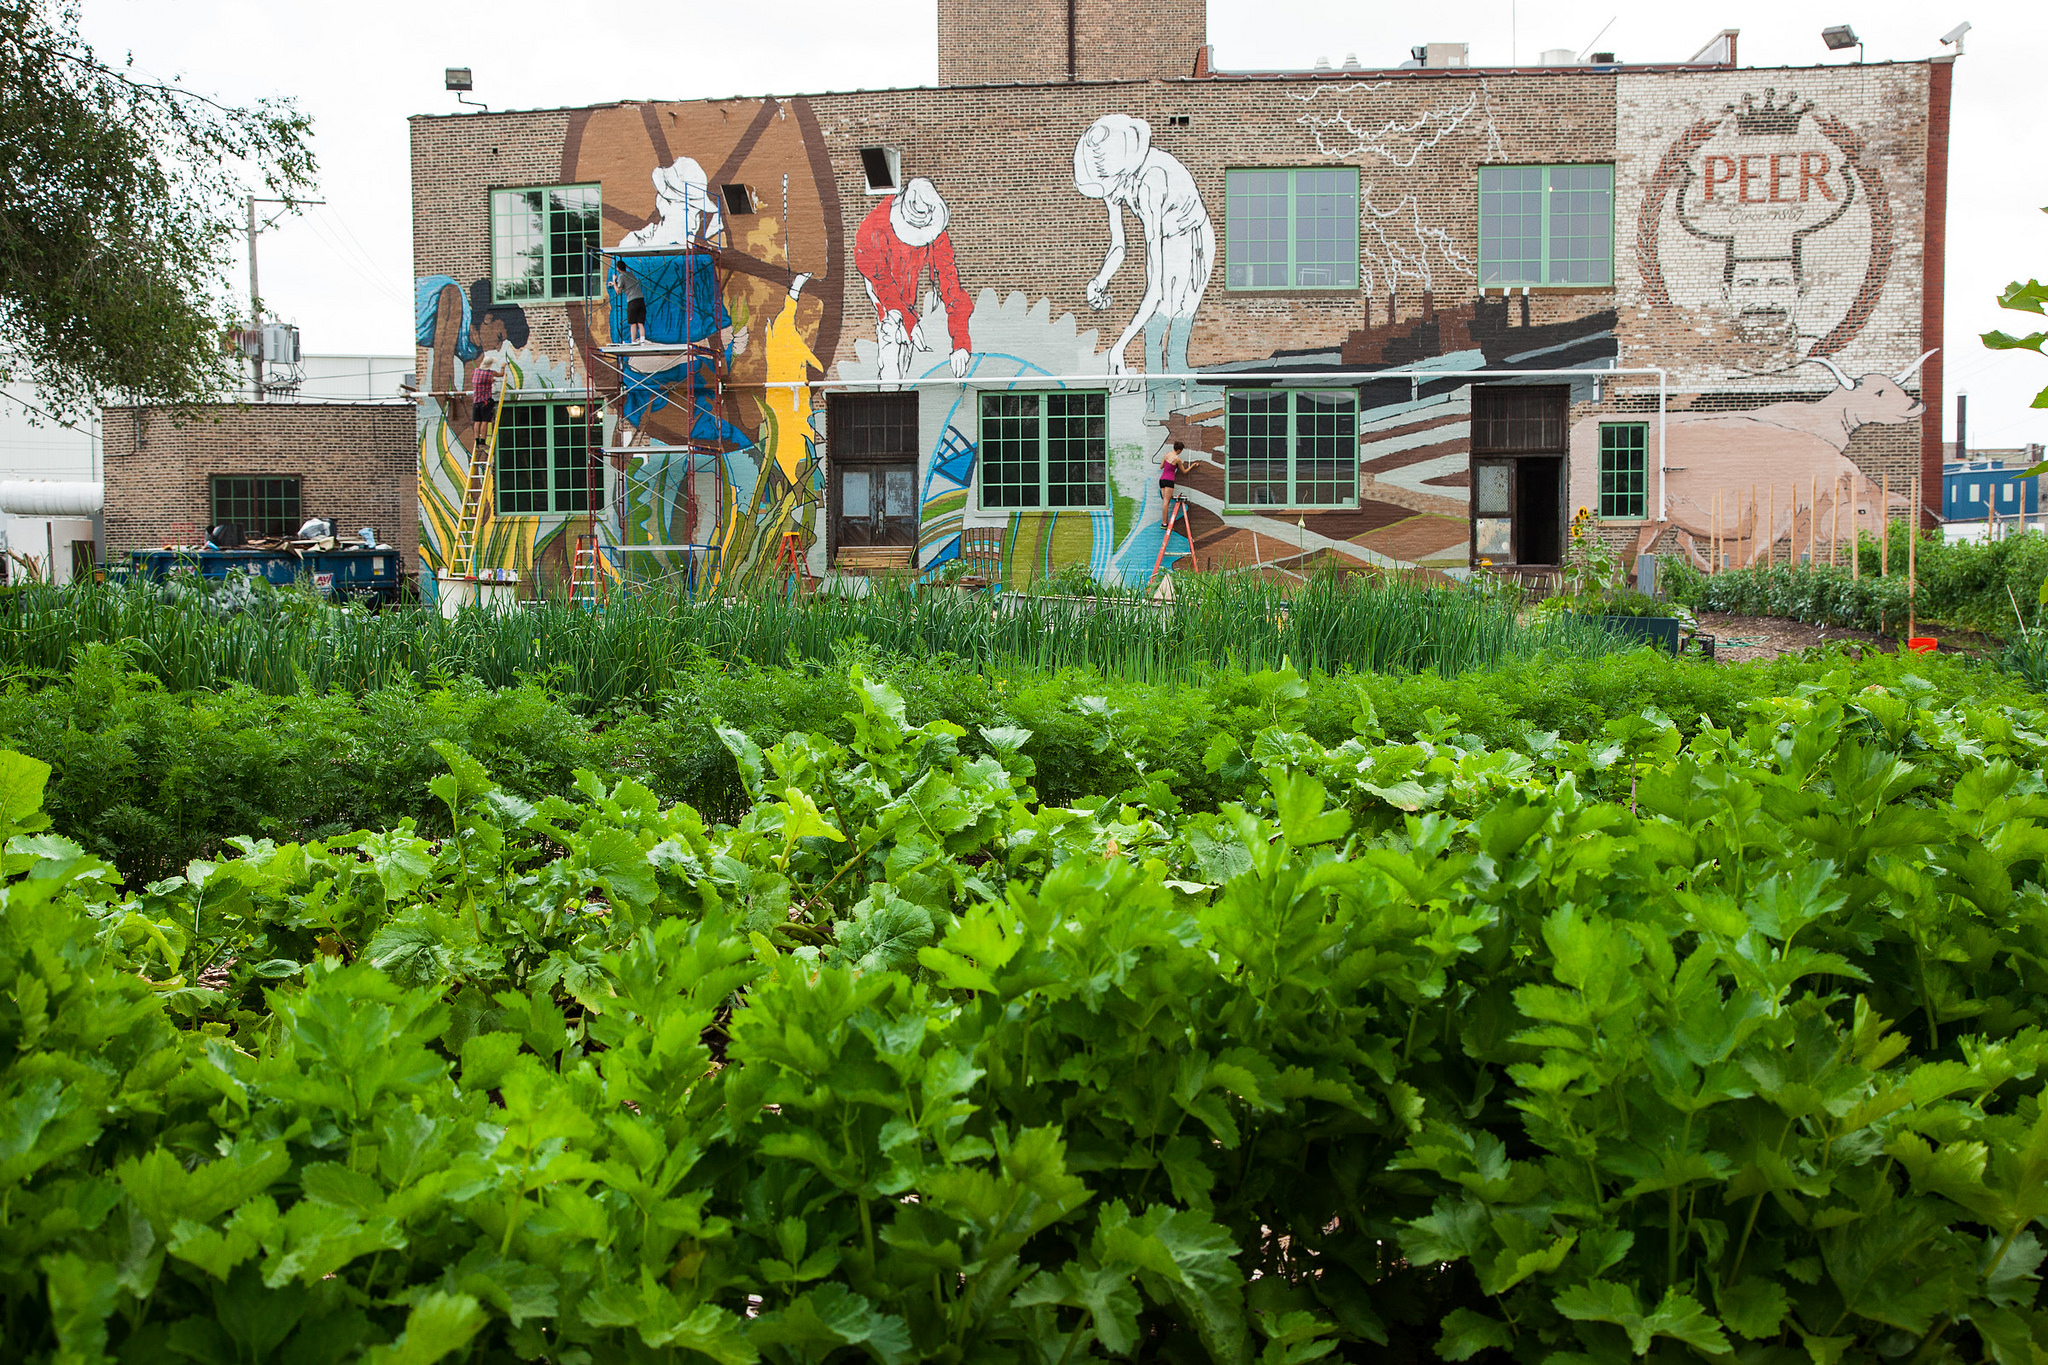
\includegraphics[width=14cm]{image_folder/the_plant_1.jpg}
    \caption{The Plant im Zentrum Chicagos}
\end{figure} 

\begin{figure}[htbp]
    \centering
    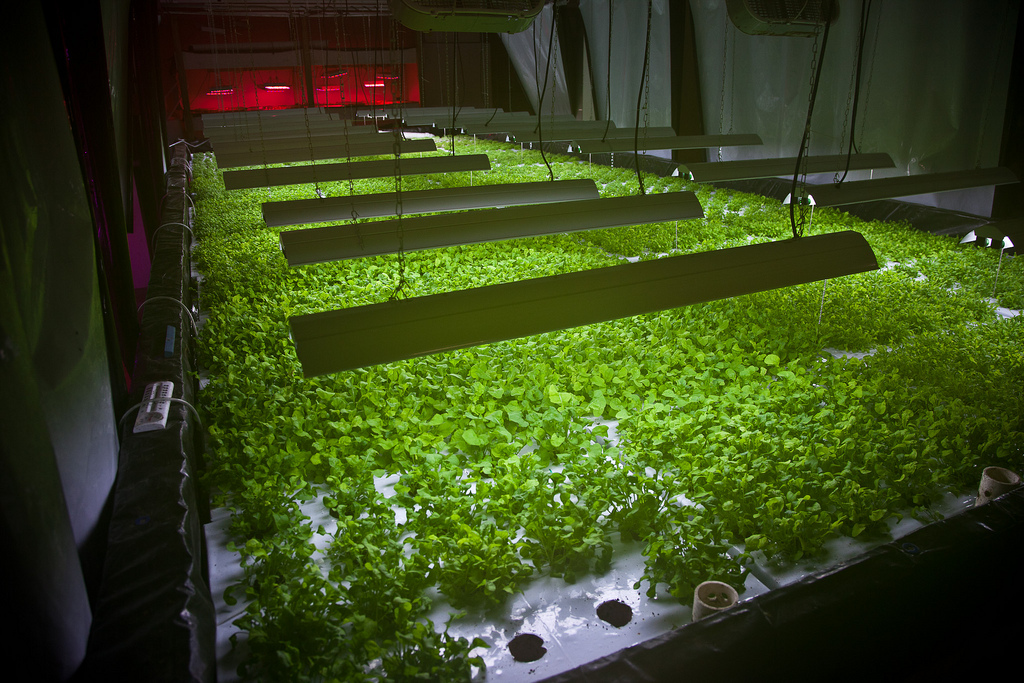
\includegraphics[width=14cm]{image_folder/the_plant_2.jpg}
    \caption{Hydroponischer Plfanzenanbau in The Plant}
\end{figure} 

\subsubsection*{The Plant (Chicago)}
Das im Zentrum Chicagos gelegene The Plant war vor seiner aktuellen Gebäudenutzung eine Fleischverarbeitungsanlage. Dank staatlicher Unterstützung wurde aus dem 8000 Quadratmeter alten Warenhaus eine energieneutrale Vertical Farm\footnote{Unter Vertical Farming versteht man eine Landwirtschaft betrieben in einem mehrstöckigen Gebäude. Nähere Informationen dazu folgen im Kapitel 10}. Das heißt auf mehreren Etagen des Gebäudes werden unter anderem Pflanzen, Gemüse und Pilze angebaut. Ergänzend dazu werden regelmäßig Kurse zum Anbau und zur Ernährung gegeben. The Plant beherbergt mehrere kleine Lebensmittelunternehmen, sowie eine Brauerei und eine Gemeinschaftsküche. Aufgrund des energieneutralen Gebäudekonzeptes ordnen Berges et. al. dieses Projekt als innovativ ein. Das Gebäude beinhaltet nämlich eine Biogasanlage, die ausreichend Lebensmittelabfall in Elektrizität und Wärme verbrennt, um das Haus zu heizen und zu kühlen.  \footcites[Vgl.][S.18]{Al-Kodmany2018TheCity} 

\begin{figure}[htbp]
    \centering
    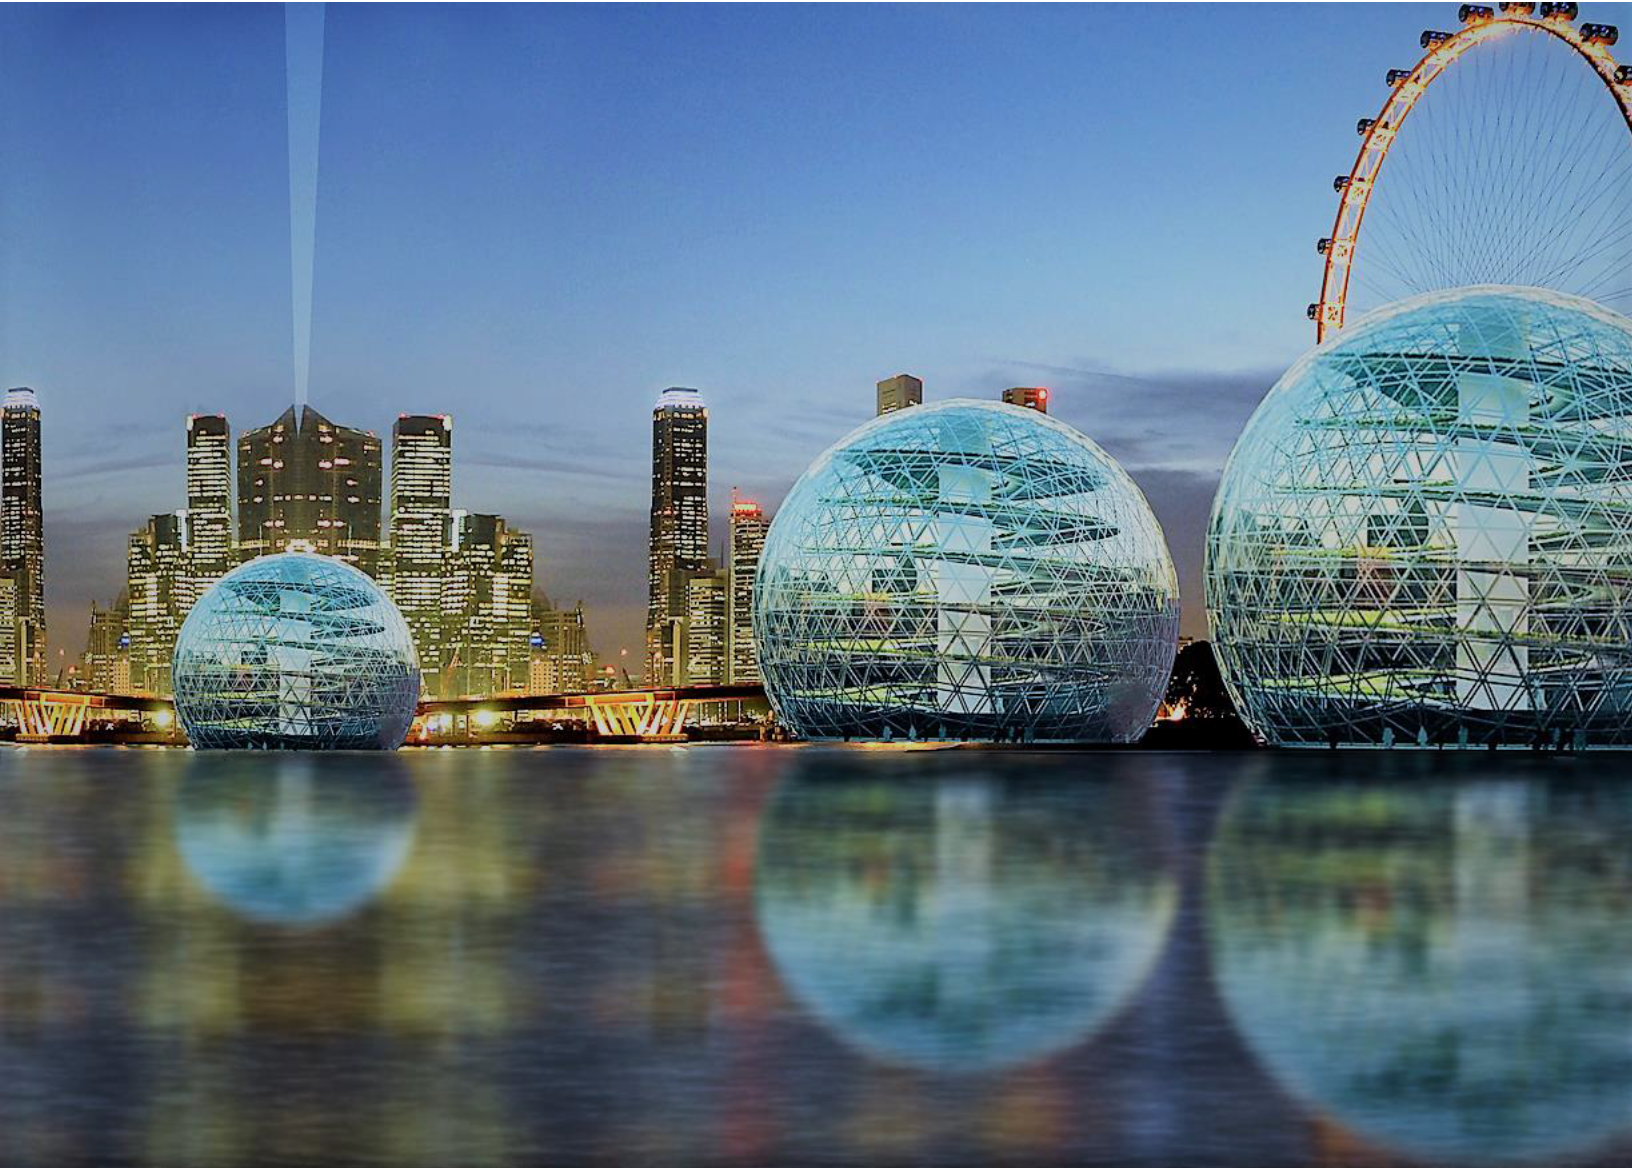
\includegraphics[width=12cm]{image_folder/plantagon.png}
  \caption{Plantagon - Erster Prototyp für tropische Städte}
  \label{fig:plantagon}
\end{figure} 

\subsubsection*{Plantagon (Schweden)}

Gegründet im Jahr 2008 in Schweden ist Plantagon ein internationales Unternehmen, das durch sein innovatives Vertikal-Farming-Gebäudekonzept viele Preise gewonnen hat.\footcite[Vgl.]{PlantagonAwardsPlantagon} Besonders innovativ sei ihr Konzept zum automatisierten Lebensmittelanbau (siehe Abbildung \ref{fig:plantagon}), das wie folgt funktioniere:\footcite[Vgl.][S.21f]{Al-Kodmany2018TheCity}  In der Mitte eines Gebäudes befindet sich eine Helixstruktur. Am unteren Ende der Helix werden von Mitarbeitern Samen in Töpfe platziert. Daraufhin werden mit Hilfe eines Aufzuges diese Töpfe am oberen Ende der Spirale befördert. Hier wird jede Pflanze entlang der Helix einzeln durch robotische Förderbänder abhängig vom Sonnenlicht, dem Alter und ihre Größe hoch und runter bewegt. Zur Ernte werden sie dann anschließend nach unten befördert. Dieses Konzept könne in drei verschiedene Gebäudeformen umgesetzt werden: Entweder integriert an einer Gebäudefassade, als multifunktionales Gebäudekomplex mit Büros, Hotels und Mietswohnungen, oder in einem alleinstehenden Gebäude, das sich ausschließlich der landwirtschaftlichen Produktivität widmet. Für die letzte Variante wurden zwei Prototypen erstellt. Der erste Prototyp (siehe Abbildung \ref{fig:plantagon}) hat die Form einer Halbkugel, der zweite Prototyp „Plantscraper“ diene als aktuelles Referenzmodell für ein VF-Konzept (siehe Abbildung \ref{fig:plantagon_2}). Es hat einen Umfang von zwölf Etagen, einen „Bauernmarkt“ im Erdgeschoss und Büroräume für weitere UL-Forschung. Ausgerichtet auf asiatische Megastädte, soll die Produktion schätzungsweise 300 bis 500 Tonnen Blattgemüse wie beispielsweise Pak-Choi produzieren. Trotz mehreren Preisen und angemeldetem Patent existiert derzeit noch kein umgesetztes Hochhaus nach diesem Konzept.

\begin{figure}[htbp]
    \centering
    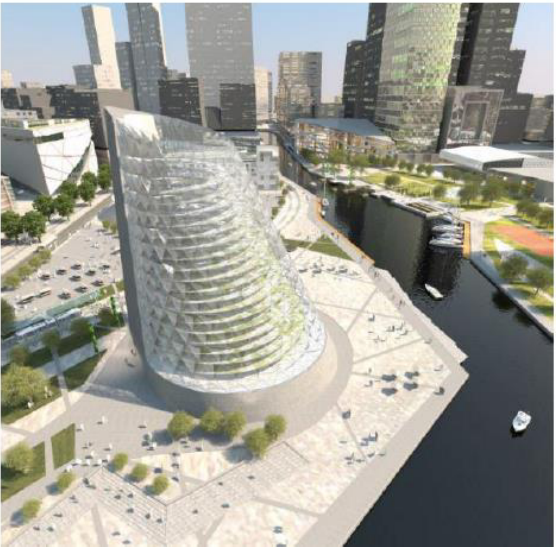
\includegraphics[width=9cm]{image_folder/plantscraper.png}
  \caption{Referenzmodell „The Plantscraper“ von Plantagon}
  \label{fig:plantagon_2}
\end{figure} 

\subsection{Aktuelle Lebensmittelversorgung in Städten***} 

„Nahrung ist eine grundlegende Basis für die Existenz menschlichen Lebens". Hiermit fasst Stierand Informationen aus von Blanckenburgs Text in Zukunft, Welternährung - Gegenwartsprobleme und Strategien" zusammen. \footcite[S.122f]{Stierand2008StadtLebensmittel} „Jeder Mensch benötigt eine angemessene Ernährung, um körperlich und geistig leistungsfähig zu bleiben. (Auch für die Aufrechterhaltung der Gesundheit und die Abwehr von Krankheiten ist ausreichende Ernährung wichtig.“ \footcite{Blanckenburg1987ZukunftDie}

Laut Stierand hat die Erzeugung und Verarbeitung von Lebensmitteln in der heutigen Zeit "ihre Bindung an die Verbrauchsräume weitgehend verloren, schnelle und gute Transportmöglichkeiten erlauben weltweiten Handel. So ist die Landwirtschaft in und um Städte nicht mehr überlebenswichtig".\footcite[S.122f]{Stierand2008StadtLebensmittel} 

\begin{figure}[htbp]
\centering
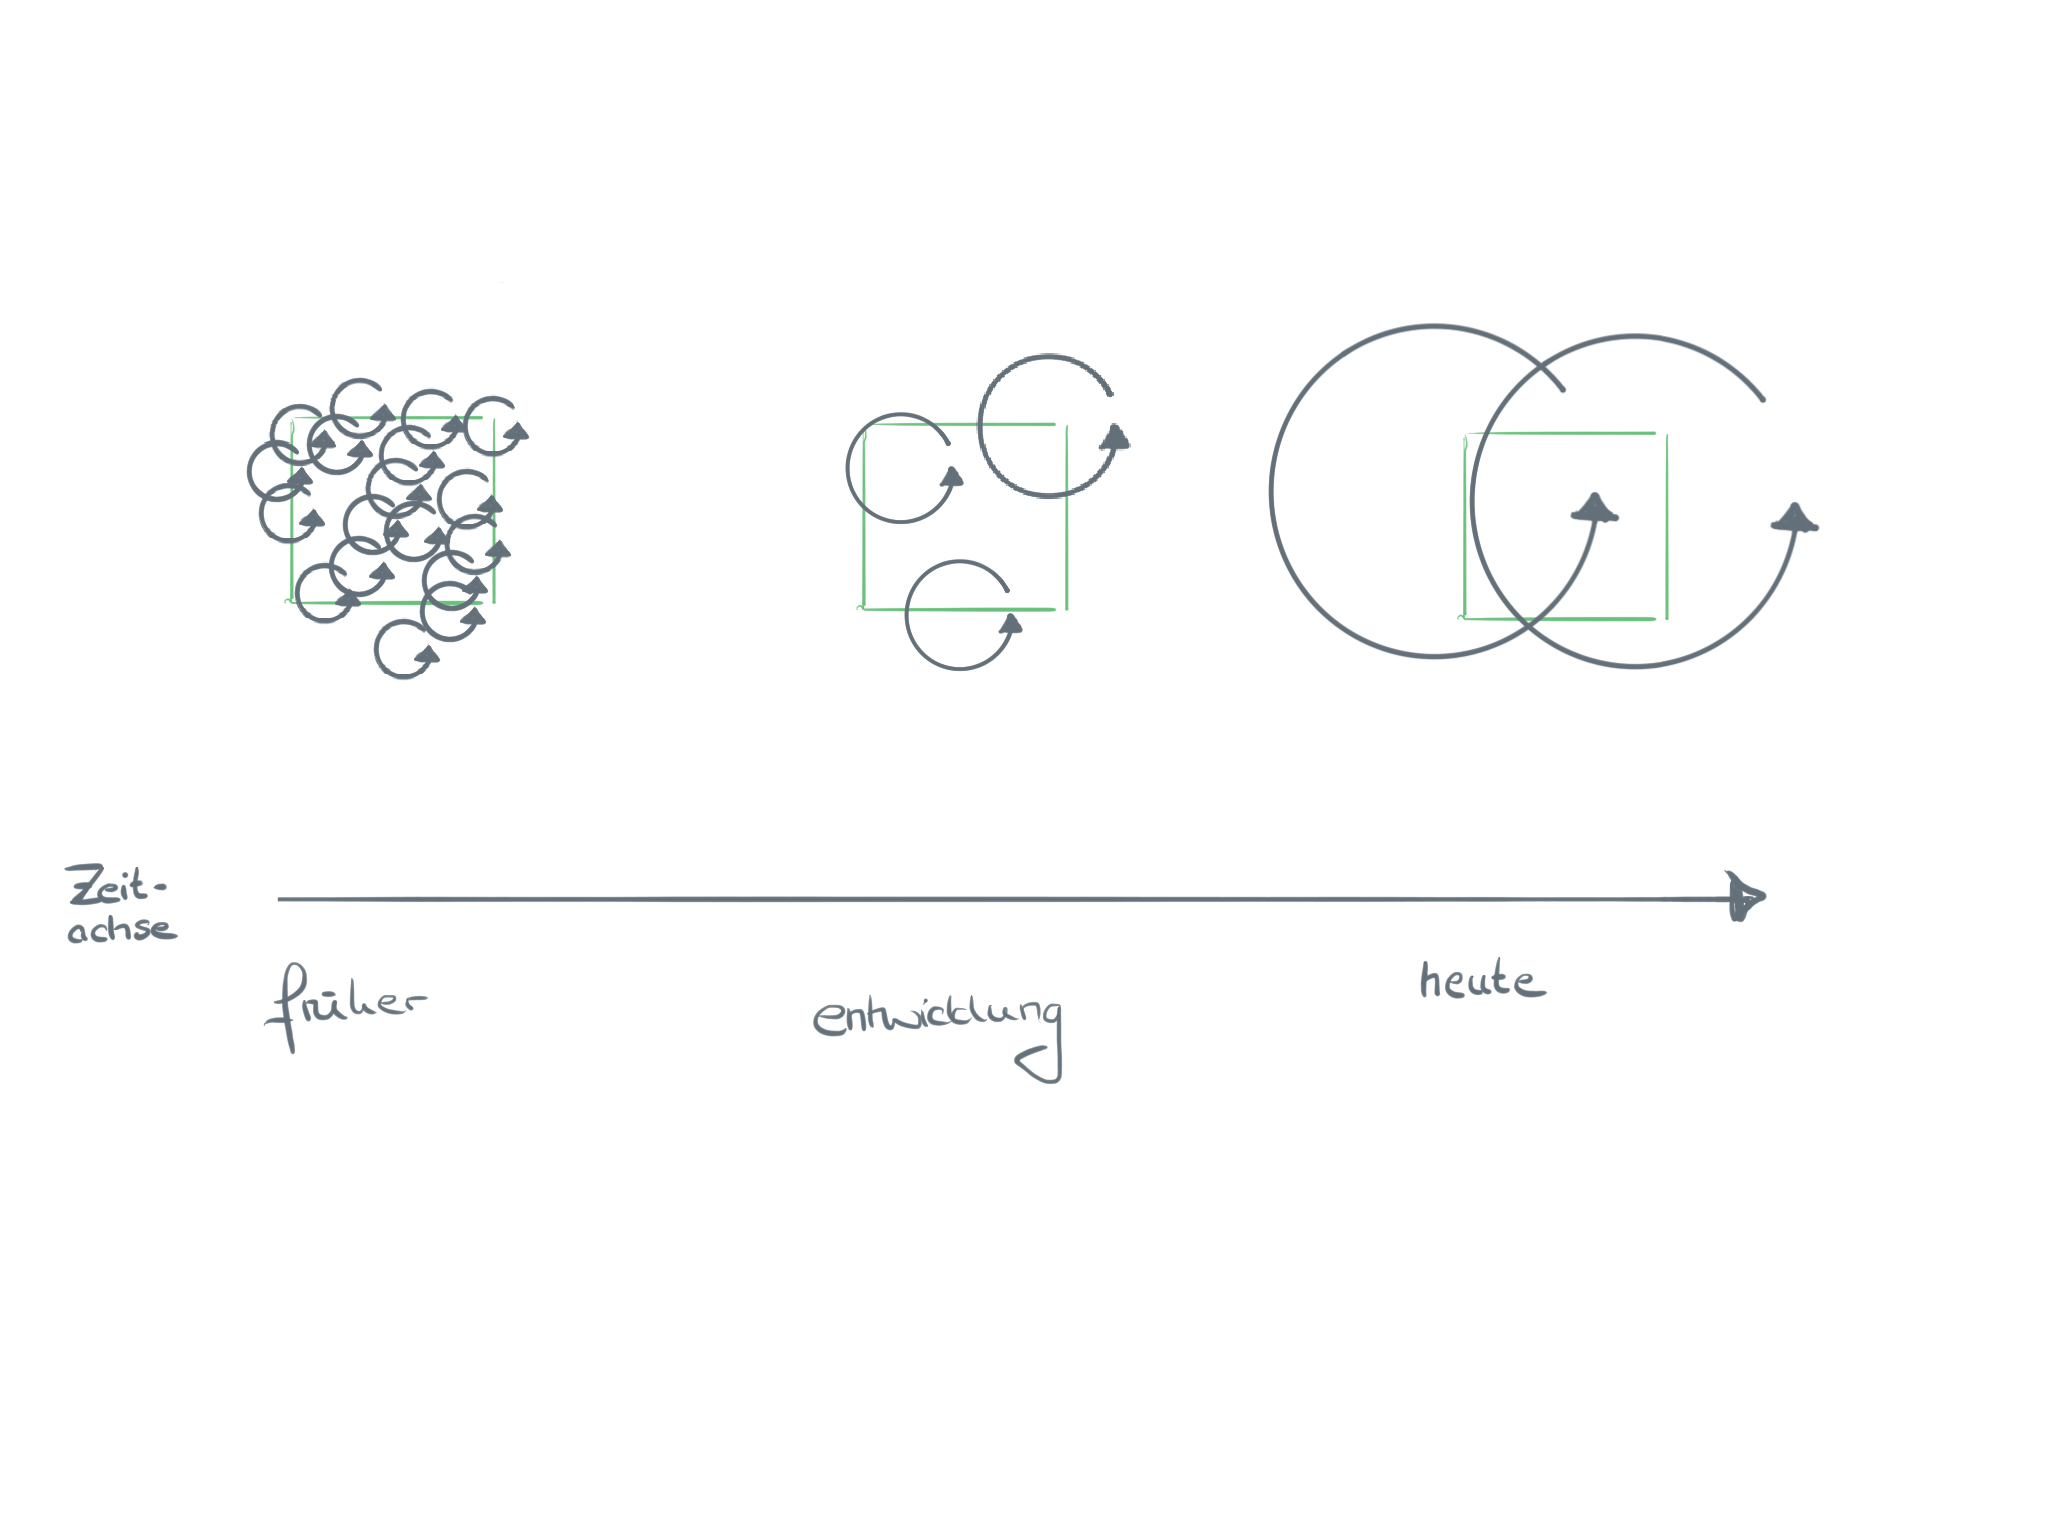
\includegraphics[width=12cm]{image_folder/ernahrung.png}
\caption{Änderung des Ernährungsmaßstabs}
\label{fig:massstab}
\end{figure}

Mit der Entstehung von regionalen und nationalen Ketten dehnte sich der Handel aus und das Ernährungssystem erfuhr eine "Delokalisation“ \footcite{MASSIMOMONTANARI1993DerEuropa}[188ff]. Diese Veränderung durch die Ausbreitung der Filialen und der folglich flächendeckenden Versorgung wirkte sich sowohl in städtischen als auch in ländlichen Regionen aus. Seitdem ist "die Bindung zwischen Wohnort und Nahrung [...]aufgehoben, die Ernährung ist nicht mehr von saisonalen Engpässen und Überschüssen abhängig.\footcite{Stierand2008StadtLebensmittel, S.122f}  

\subsubsection {Ernährung in der Stadt}
Heute erreichen Lebensmittel den Konsumenten zu 90\% in verarbeiteter Form. Vor allem der Anteil von „Convenience Produkten“, also Fertig- oder Halbfertigprodukten habe laut Hemmerling stark zugenommen. (Hemmerling et al., 2012, p. 33). „Die zeitaufwendigen Prozesse der Verarbeitung und Zubereitung wurden zunehmend in die Industrie transferiert.“  
Die dauerhafte und bewusste Essensplanung bezüglich saisonaler Verfügbarkeit von Lebensmitteln wurde durch den globalen Handel und die folglich beinahe ständige Verfügbarkeit der Lebensmittel überflüssig.\footcite[Vgl.][S.20]{SchmidtDieVon}
Laut Stierand wurde der Mensch erst durch das moderne Ernährungssystem zum ausschließlichen Verbraucher von Lebensmitteln. Er begründet dies mit der Aussage: "Wir sind Konsumenten. Wir essen nicht mehr selbstgezogene Lebensmittel, sondern wir verzehren Produkte, deren Herkunft, deren Produktion und Geschichte uns nur in Ausnahmefällen bekannt ist. Essen als Resultat einer arbeitsteiligen Nahrungskette […] wird uns fremd, zumindest aber fremder."\footcite{Spiekermann2000GesundeKulturwissenschaft} 
"Die Mehrzahl der heutigen Konsumenten habe weder direkten Kontakt zu den ursprünglichen Erzeugern, noch haben sie einen Einblick in die Prozesse der Verarbeitung und Zubereitung.
Die Ernährung beginnt für die meisten im Warenregal von Supermärkten, Fachgeschäften oder Discountern" (BMEL, 2014).\footcite[S.20]{SchmidtDieVon}\footcite[Vgl.]{BerichtInhalt}

 Auf eine detailierte Beschreibung der Essgewohnheiten der städtischen Bewohner in der heutigen Zeit kann in diesem Rahmen nicht eingegangen werden. Im folgenden wird daher versucht die Hauptentwicklungen bezüglich der Nachfrage an Lebensmittel am Beispiel Deutschland aufzulisten. 
 
 \begin{itemize}
\item Convenience-Produkte: "Fertig- und Halbfertiggerichte haben sich bereits so fest in unserer Ernährung etabliert, dass sie nicht mehr als solche wahrgenommen werden: Nudeln und Joghurt kommen zu fast 100\% aus industrieller Produktion, auch Brot wird in fast keinem Haushalt mehr selbst hergestellt. [...] Bestimmte Fertigprodukte (wie zum Beispiel der Hamburger)
haben eine eigene Identität bekommen, bei ihnen denkt niemand mehr an die eigentlichen Rohprodukte." \footcite{Escher2003EssenKultur}
\item Funktionelle Lebensmittel: Darunter werden Produkte definiert, die über ihre Nährstoffe hinaus eine gesundheitsfördernde Wirkung haben. \footcites[Vgl.][S.5]{Heasman1958-2001TheProfits}"Prominentes, aktuelles Beispiel sind probiotische Joghurts, die durch spezielle Joghurtkulturen eine Steigerung der Abwehrkräfte versprechen."\footcite[S.14]{Stierand2008StadtLebensmittel}
\item Produkte aus ökologischem Anbau: In Deutschland leben "40\% der Bio-Käufer [...] in Großstädten, 27\% in mittleren und 33\% in kleineren Städten beziehungsweise Orten."\footcite[S.14]{Stierand2008StadtLebensmittel}
\end{itemize}
D. Schmidt fasst die Veränderungen in der Lebensmittelversorgung wie folgt zusammen. Die Folgenden Punkte beziehen sich dabei auf städtische und ländliche Bewohner in Industrieländern. (Da sich (wie oben genannt) seit der Entstehung der Filialen die ländliche und städtische Versorgung einander angeglichen hat.)

\begin{itemize}
\item Die "Ernährung kann gesichert werden ohne selbst als Produzent tätig werden zu
müssen.\footcite[S.20]{SchmidtDieVon}
\item Arbeitsverhältnisse sind unabhängig von der häuslichen Versorgung.
\item Saisonale oder regionale Verfügbarkeiten werden durch den globalen Handel
ausgeglichen, so dass nahezu jederzeit alle Lebensmittel zur Verfügung stehen.
\item Lebensmittel verarbeiten und zubereiten zu können ist keine Notwendigkeit für
eine (warme) Mahlzeit.
\item Die städtische Ernährung und die ländliche Ernährung unterscheiden sich nicht"\footcite[S.20]{SchmidtDieVon}
\end{itemize}



\subsubsection{Die Rolle des Konsumenten}


Seit der allgegenwärtigen Verfügbarkeit von Lebensmitteln, bleibt dem Konsument hinsichtlich seiner Ernährung, lediglich die Aufgabe, sich zwischen der Vielzahl von Produkten zu entscheiden. Gemäß Schmidt appelliert der Handel ab diesem Punkt an die Ernährungskompetenz des informierten Bürger.\footcite[S.20]{SchmidtDieVon} "Seit der Proklammierung der Agenda 21 (UN, 1992) wird erwartet, dass der Verbraucher die Nachhaltigkeit seines Ernährungsverhaltens bedenkt."\footcite[S.20]{SchmidtDieVon} Gemäß Reisch ist nachhaltiger Konsum "die Abwägung vieler Faktoren". 
Sustainable food consumption is a choice for food, which is beneficial and life enhancing for individuals, society and the planet. \footcite{article}
Die Verantwortung die der Konsument schlussendlich übernimt ist laut Schmidt sowohl persönlich als auch global.\footcite{SchmidtDieVon}

Zwar besteht die Bereitschaft vieler Menschen mehr Geld für eine nachhaltige Ernährung auszugeben.
(Rödiger \& Hamm, 2015),
(Feldmann \& Hamm, 2015) Gleichzeitig überschätzen sich die Konsumenten diesbezüglich, da sie überhaupt nicht mehr fähig sind, zwischen den Risiken und Auswirkungen auf ihre Ernährung sowie die ökologische Entwicklung der Umwelt zu unterscheiden und diese zu bewerten. \footcite [vgl] (Rödiger \& Hamm, 2015; Feldmann \& Hamm, 2015; Stierand,
2008, p. 121; Verbeke et al., 2007; Röhr et al., 2005).

\section{Formen der urbanen Landwirtschaft}

Im Rahmen dieser Forschung wurden einige Beispielprojekte untersucht bezüglich ihres Beitrags zur nachhaltigen Entwicklung. Im Folgenden werden die Ergebnisse aufgelistet.

Gemäß Al-Kodmany versprechen technische Entwicklungen wie Hydrophonik Aeroponik und Aquaponik eine große Entwicklung in der Zukunft des vertikalen Anbaus und im Bereich der Gewächshaustechnologie. 

\begin{displayquote}
"recent advantages in greenhouse technologies such as hydroponics, aeroponics,and aquaponics have provided a promising future to the vertical farm concept."\footcite[S.1]{Al-Kodmany2018TheCity}\end{displayquote}

Al-Kodmany vertritt die Ansicht, der Erfolg von Großprojekten wie Hochhaus-Farmen hänge schlussendlich vom Erfolg der mittelgroßen Farming-Projekte und der Entwicklung ihrer Technologien ab.\footcite[Vgl.][S.2ff]{Al-Kodmany2018TheCity}

\begin{itemize}
    \item BIA: buidling-integrated-agriculture = Kombination aus Anbau-System integriert auf  Gebäude: Synergien zwischen Gebäude und  and Agrikultur (beispielsweise Energieerzeugung oder Lebensmittel) werden möglich
    \item ZFarming: Zero-acreage farming = Urbane Agrikultur, welche keine landwirtschaftliche Fläche des Erdbodens benötigt: Rooftop-Garden, rooftop greenhouses, edible green walls aber auch indoor farms und vertikale greenhouses
    \item Indoor Farming Systems (Farmscraper) = Die Bereitstellung von saisonunabhängigem und damit ganzjährig züchtbaren Nahrungsmittel ist einer der genannten Hauptvorteile von Indoor Farming. Zusätzlich werden die Nahrungsmittel dabei vor äußeren EInflüssen wie Witterungseinflüsse, Krankheits- und Schädlingsbefall geschütz.\footcite{Schulz2013UrbaneLandmanagements} Gemäß der Autoren erscheint "Besonders im Hinblick auf prognostizierte Wetterextreme im Zuge des Klimawandels und der besonderen Betroffenheit der Landwirtschaft [...] das isolierte Wirtschaften vorteilhaft.\footcite{Schulz2013UrbaneLandmanagements}
\end{itemize}


\begin{figure}[htbp]
\centering
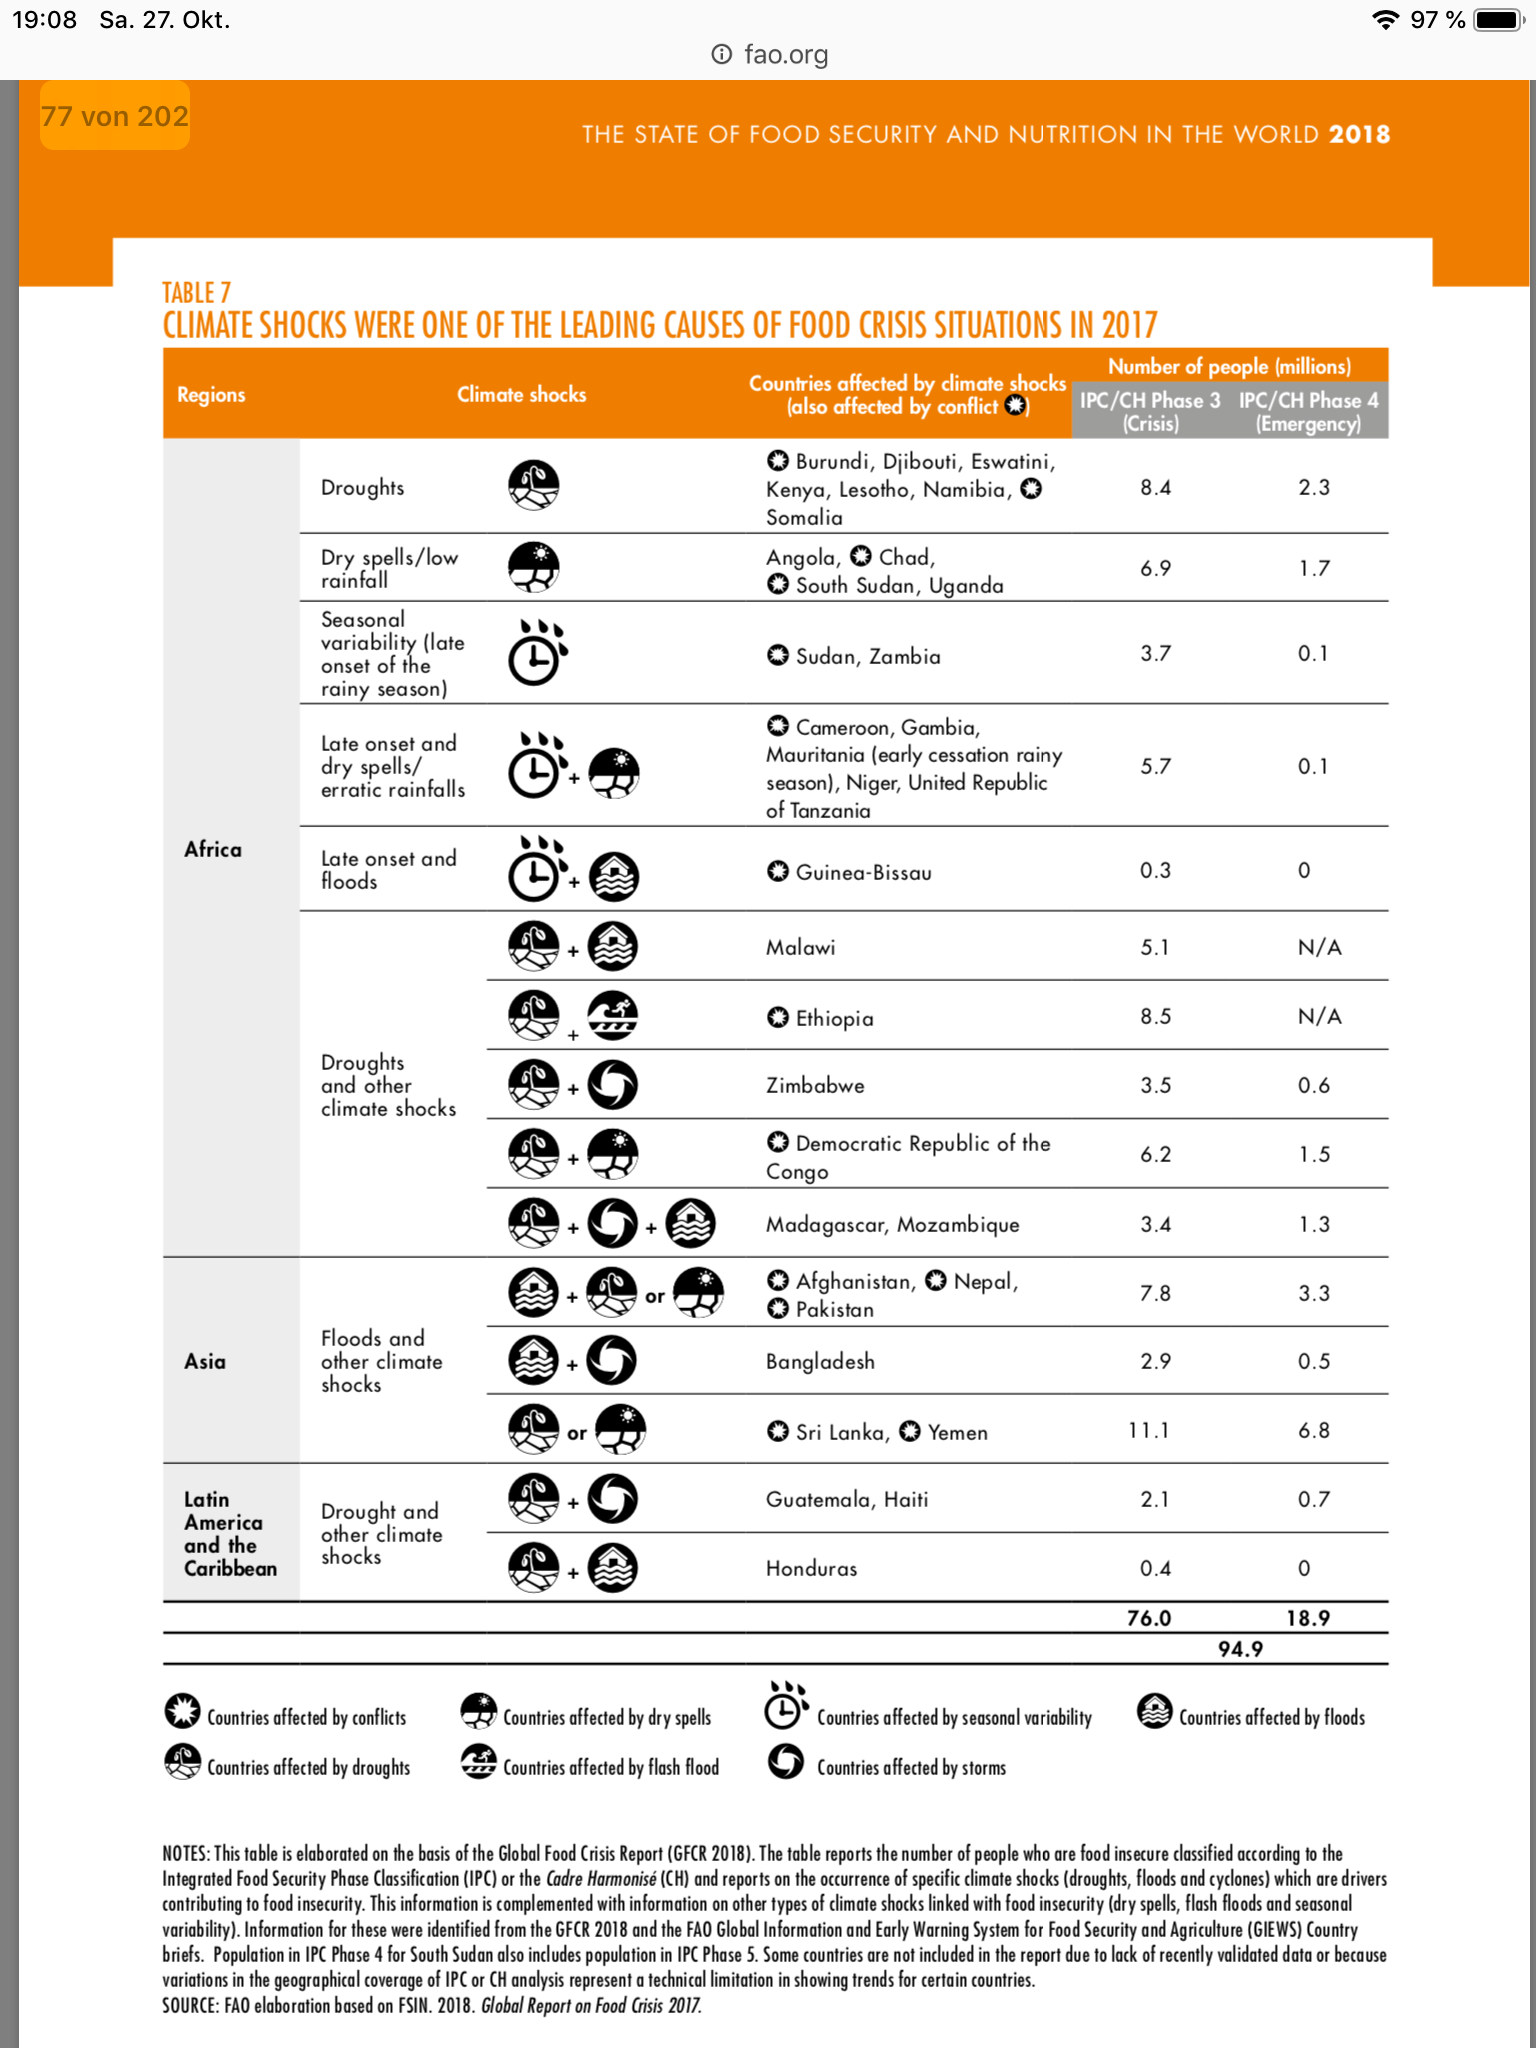
\includegraphics[width=10cm]{image_folder/beeintrachtigungklima.png}
\caption{Beeinträchtigungen der Nahrungsmittelversorgung durch Klimakatastrophen im Jahr 2017}
\label{fig:Die Grafik visualisiert den Zusammenhang zwischen Klima und Versorgung: Beeinträchtigungen der Nahrungsmittelversorgung durch Klimakatastrophen im Jahr 2017}
\end{figure}
   

\subsection{Vertikale Landwirtschaft}

Grundsätzlich wird vertikale Landwirtschaft in drei Typen unterteilt:\\ 

1. Vertikale Hängegärten \newline
2. Rooftop Farming: Dies impliziert die Nutzung von Hochhausdächern oder die Integration von Anbau in bestehende Gebädestrukturen (z.B Restaurant oder Supermärkte), welches diesen eine zweite Funktion verleiht.\newline
3. Kommerzieller, großflächiger Anbau über mehrere Etagen.

\subsubsection{Hydroponik und Aeroponik}
Laut Möller haben diese beiden Technologien den Umgang mit der Ressource Wasser in der Landwirtschaft auf ein neues Level gebracht. Die Kombination beider Technologien in einem Kreisslaufsystem kann bis zu 95 \% des Wasserverbrauchs einsparen.

\begin{figure}[htbp]
\centering
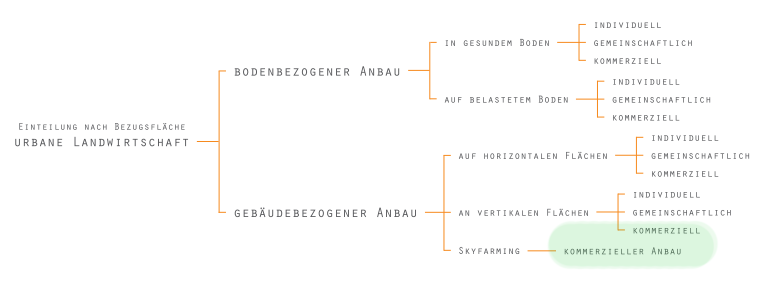
\includegraphics[width=6cm]{image_folder/moglicheEinteilungena_s32.png}
\caption{Fokussierung auf Vertikales Indoor Farming}
\label{fig:Fokussierung auf Vertikales Indoor Farming}
\end{figure}

\subsubsection{Sky Greens in Singapur}

Singapur besitzt im Verhältnis zu seiner Einwohnerzahl (5 Millionen)  eine relativ geringe Fläche. Demnach geht es davon aus, in den kommenden Jahren mit Nahrungsmittelmangel zu kämpfen. 
Nur etwa 7\% der Nahrungsmittel die dort konsumiert werden, wurden auch tatsächlich in Singapur produziert. Nur 250 Acker auf der Insel widmen sich dem Anbau von Nahrungsmitteln. Der weitere Lebensmittelbedarf wird über Import gelöst. Aus den oben genannten Gründen hat Singapur viel Mühe in die Forschung des Lebensmittelanbaus mittels Vertical Farming gesteckt. 
\begin{displayquote}
The five-year-old farm is 3-stories tall (9 m or 30 ft) and uses a method called “A-Go-Gro (AGG) Vertical Farming” that utilizes translucent green houses to grow tropical leafy vegetable year-round at significantly higher yields than traditional farming methods. Sky Greens is capable of producing one ton of fresh veggies every other day. It supplies a variety of tropical vegetables including Chinese cabbage, Spinach, Lettuce, Xiao Bai Cai, Bayam, Kang Kong, Cai Xin, Gai Lan and Nai Bai. By providing high-quality produce at relatively affordable costs, the farm has thrived and intends to expand its production, providing a wider variety of vegetables.\footcite[S.15]{Al-Kodmany2018TheCity}
\end{displayquote}

\begin{figure}[htbp]
\centering
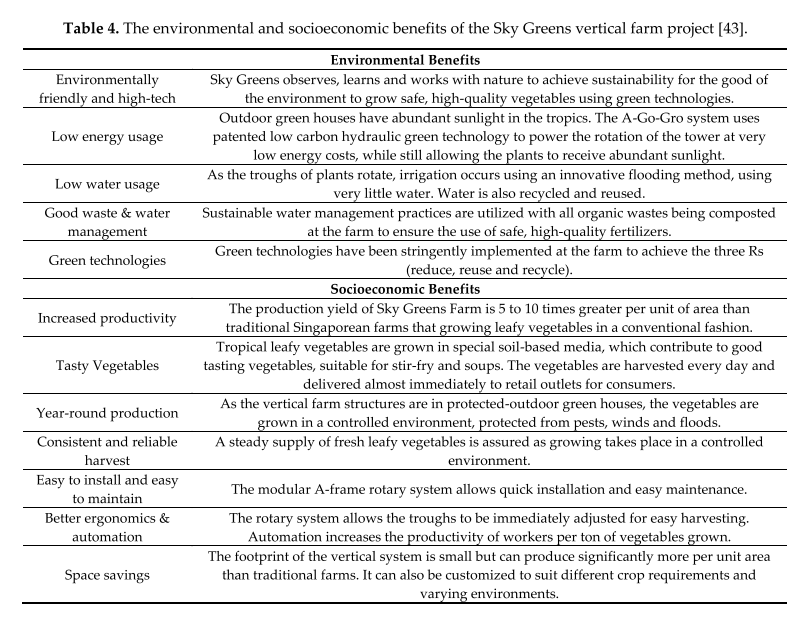
\includegraphics[width=14cm]{image_folder/skygreenbenefits.png}
\caption{Positive Auswirkungen von Sky Green }
\label{fig:Positive Auswirkungen von Sky Green}
\end{figure}

\subsubsection {Nachhaltigkeitsbewertung von VF}
\subsubsubsection{Vorteile von VF}

Vertical Farming Systeme können ganzjährig Nahrungsmittel produzieren und sind durch ihre Abgeschlossenheit unabhängig vom Jahreswechsel oder Klima-Extremen. Gleichzeitig besteht durch die integration von neuen Technologien, die Möglichkeit einen höheren Ertrag pro Fläche zu erzielen. Da auf mehreren Stockwerken angebaut wird, entsteht eine Dreidimensionalität, die es ermöglicht, den Ertrag pro Quadratmeter je Stockwerk zu maximieren.\footcite{Despommier2010TheCentury.} Zusätzlich soll der Verbrauch von Trinkwasser wird minimiert indem die Wurzeln direkt bewässert werden und die Verdunstung gesenkt wird. Einige VF-Systeme können sogar Grau- und Schwarzwasser wiederverwenden, welches Abwasser in sowie Toilettenabwasser bedeutet. 

Ebenso ist die Gefahr bei vertikalen Farmen geringer, dass Bakterien im großen Stil über die Erde weitergegeben werden.

\begin{displayquote}
„Vertical farming meets the needs of an increasing urbanization. Buildings used for farming can be placed anywhere while outdoor fields are static in location. By strategically placing vertical farms inside or in the near vicinity of urban centers and cities, we are able to meet the need for localization of food production. Foods can be harvested and sold in the same building immediately after harvest, eliminating the need for transportation and storage.”\footcite[S.7]{PeterMollerVoss2013VerticalRise}
\end{displayquote}

\begin{itemize}
\item Ortsunabhängigkeit, denn VF eignet sich besonders um die Problemen der steigende Verstädterung zu mildern. VF Fabriken können ortsunabhängig gebaut werden, während  ländwirtschaftliche Flächen orts- und bodenqualitätsgebunden sind.
    \item Lokalisierung der Lebensmittelproduktion, was Transport und unnötige Lagerung unnötig macht. In einem weiteren Schritt kann daran gedacht werden, nach Bedarf zu ernten, was unnötige Lagerung oder Lebensmittelabfall zusätzlich reduzieren könnte.
\end{itemize}

Im Vergleich zu traditionellen und landbasierten Anbaumethoden, die für Traktoren, Pflüge etc. fossile auf fossile Energien angewiesen sind. Als Beispiel: In Nordamerika wird 20\% der fossilen Energie von der Landwirtschaft verbraucht.\footcite[Vgl.][S.27]{Al-Kodmany2018TheCity[82,83}, kann VF den Bedarf an fossilen Rohstoffen senken.
Hinsichtlich des Transports schneidet VF im Vergleich zu traditioneller Landwirtschaft ebenso besser ab. Die Distanz zwischen Herstellung und Konsum wird in den meisten Fällen wesentlich kleiner. Als Orientierung: Lebensmittel aus traditionellem Anbau legen im Durchschnitt 15500 Meilen (ungefähr 2400 Km) zurück.


\subsubsubsection{Herausforderungen von VF}

Sofern die Idee von VF darin besteht Nahrungsmittelproduktion zu lokalisieren, muss das VF dementsprechend zentral in der Stadt platziert sein. Eine der größten Herausforderungen, die sich hierbei für die Planer von VF - Projekten ergibt, ist die Verfügbarkeit von erschwinglichem Bauplatz in der Stadt. So scheitern laut Möller viele der Projekte vor dem Start aufgrund von fehlenden finanziellen Mitteln.\footcite[S.8]{PeterMollerVoss2013VerticalRise}

Häufig ist die Akzeptanz für Indoor Vertikal Farming bei den Stadtbewohnern noch nicht vorhanden, da diese nicht mehr an die Landwirtschaft erinnert, die sie zuvor kannten.


\begin{figure}[htbp]
\centering
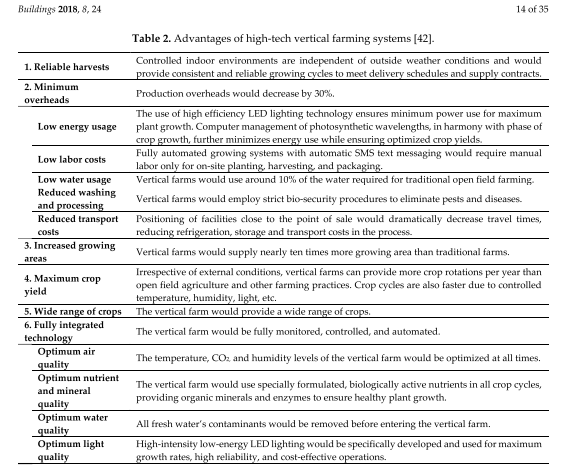
\includegraphics[width=14cm]{image_folder/moglicheVorteileVonVF.png}
\caption{mogliche Vorteile von Vertical Farming Systemen im Überblick}
\label{fig:vorteileVF}
\end{figure}



\begin{figure}[htbp]
\centering
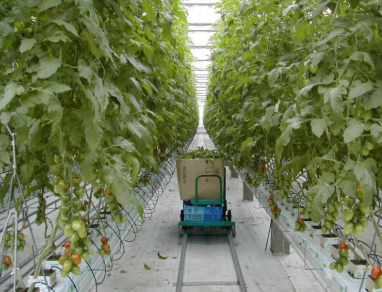
\includegraphics[width=14cm]{image_folder/automatisation_kondo.png}
\caption{Eine Ernte-Roboter bei der Arbeit}
\label{fig:Automatisierung}
\end{figure}



\subsubsubsection{Bewertung}
Sparsamer Umgang mit Ressourcen von Anbau bis Konsum\\
Möller Voss bezieht sich in seiner Examensarbeit auf die Aussage Despommiers.\footcite[S.9]{PeterMollerVoss2013VerticalRise} Demnach bestehe durch eine Nutzung von Regenwasser oder städtischen Grauwassers für vertikale Farmen die Möglichkeit autark im Bereich der Wassernutzung zu werden.\footcites[Vgl.]{Despommier2010TheCentury.} Diese Aussage sollte allerdings mit Abstand betrachtet werden, da der nötige Energieaufwand für die Technologie der Wasseraufbereitung schlussendlich entscheidet, ob unter dem Strich Ressourcen eingespart werden.\\
\\
Kreislaufsystem\\
Biomasse die bereits zur Wiederaufbereitung von Wasser verwendet wurde, sowie weitere Pflanzenabfälle können als Biokraftstoff zur eigenbetreibung und Betreibung weiterer Farmen verwendet werden.\footcites[Vgl.][S.80ff]{Despommier2009TheFarms}\\
\\
\\
VF erfüllt die Kriterien der Nachhaltigkeit unter folgenden Bedingungen:
Für den Anbau und die Produktion muss regenerative Energie genutzt werden. Erst so kann die Ressourceneffizienz der Lebensmittel im Vergleich zu Nahrung aus konventionellem Anbau reduziert werden. 
Im Idealfall sollte also eine VF kostengünstig gebaut werden, dauerhafte und sichere Arbeitsbedingungen schaffen und unabhängig von externen finanziellen Förderungen oder anderer Unterstützung, damit eine langfristige und unabhängige Nahrungsmittelproduktion bürgernah und zentral bestehen kann.\footcite{Despommier2010TheCentury.}

\begin{displayquote}
„Working within the framework of these calculations, one vertical farm with an architectural footprint of one square city block and rising up to 30 stories (approximately 3 million square feet) could provide enough nutrition (2,000 calories/day/person) to comfortably accommodate the needs of 10,000 people employing technologies currently available.” 
\end{displayquote}

Despommier behauptet, dass unter diesen Umständen eine VF mit 30 Stockwerken, heutiger Technologie und der Größe von einem Block bis zu 10.000 Menschen versorgen könnte.\footcite{Despommier2010TheCentury.}


\subsection{Indoor Farming Systems}

Das Konzept der Landwirtschaft innerhalb von Gebäuden ist eine gängige Methode Nutzpflanzen vor Witterung und Schädlingen zu schützen. Hier werden Pflanzen innerhalb von oft technologisch weit entwickelten Gebäuden unter Anwendung von aufwändigen Bewässerungssystemen und LED-Licht herangezogen. Das Verfahren wird oft mit dem Konzept des Vertical Farmings kombiniert um noch mehr Platz zu sparen. Das Indoor Farming spielt eine immer größere Rolle in der heutigen Zeit, da Planzen an fast allen Orten der Welt angebaut werden können und das unabhängig von Klima und Sonnenstrahlung. \footcite[14.10.2018]{ACHTUNG}

\subsubsection{Growing Underground in London}

Im londoner Stadtteil Clapham befindet sich die erste Untergrund-Farm der Stadt. Diese liegt 33 Meter unter London und wurde in einem Lufschutzbunker des zweiten Weltkriegs von den Gründern  Richard Ballard, Steven Dring und Michel Roux Jnr eingerichtet. Die Farm baut sogenanntes Mikrogemüse an welches nach nur wenigen Tagen abgeerntet wird. Die Anbaufläche beläuft sich dabei auf ca. 10000 Quadratmeter und die Farm produziert laut Angaben des Unternehmens ca. zwischen 5.000 und 20.000 Kilo Lebensmittel pro Jahr. Herangezogen werden die Planzen mit LED-Licht und für die Bewässerung sorgt ein hydroponisches Bewässerungssystem, welches laut dem Unternehmen ca. 70 Prozent weniger Wasser verbraucht als herkömmliche Anbauformen auf dem Land. Die Fläche des Schutzbunkers blieb bis zur Einrichtung der Farm ungenutzt weswegen keine weitere Fläche erschlossen werden musste. Pestizide und Klima spielen für diese Anbauform keine Rolle da ein eigenes Klima und Ökosystem innerhalb der Räume herrscht. Unterstützung erhält das Projekt durch die Universität Cambridge welche die Daten zur Feuchtigkeit, Temperatur und Wachstumsgeschwindigkeit wissenschaftlich auswertet.



\subsubsection{Aquaponik}
Aquaponik ist ein Kreislaufsystem, das Spring zufolge Aquakultur(Fischzucht) mit Hydroponik vereint \footcite[Vgl.][S.44f]{Spring2012DerBasel-Stadt}. Hydroponik bezeichnet eine Anbaumethode, die anstelle von Erde Substrate wie zum Beispiel Bimsstein zum Pflanzenanbau verwendet. Durch die Fäkalien der Fische werden Pflanzen gedüngt. Diese wiederum reinigen das Wasser, was zu den Fischen geleitet wird (Siehe Abbildung \ref{fig:aquaponik}). \\
\\
Turcios et. al. nach existiere diese Anbaumethode bereits vor 8000 Jahren. Erste Aquaponiksysteme seien im Süden Chinas und Thailand zu finden, wo sie Reisfelder mit Fischzucht kombinierten. Ein weiteres Beispiel sind die von den Azteken entwickelten „Chinampas“, künstliche Anbaufläche in flachen Seen.\footcite[Vgl.][S.838]{Turcios2014SustainableFuture} Erste wissenschaftliche Untersuchungen zu dieser Anbaumethode entstanden laut Diver in den achtziger Jahren an der North Carolina State University.\footcite[Vgl.][S.4]{Diver2006Aquaponics-IntegrationAquaculture} 
Ihm zufolge habe dieses System viele Vorteile. Zum einen stellt Diver fest, dass Wasserresourcen geschont werden. Für die Fischzucht war in diesem Fall nur 1 \% der Wassermenge konventioneller Zucht erforderlich. Daher eigne sich das System besonders für klimatisch trockene Gebiete. Auch die Kosten würden geringer ausfallen. Laut Experimenten an der University of Virgin Islands konnte von den aquaponischen Systemen ein vielfaches mehr an Gemüse geerntet werden als bei feldbasiertem Anbau.\footcite[Vgl.][S.7f]{Diver2006Aquaponics-IntegrationAquaculture}  \\
\\Gleichzeitig gibt es eine Reihe an Herausforderungen im Bereich der Aqua- und Hydroponik. Wegen des bestehenden Kreislaufssystems sei der Einsatz von Pestiziden Frei et. al. nach verboten.\footcite[S.43]{FreiMatthiasHartmann2007AquaponikGemuse.}  So bestehe laut Spring eine hohe Anfälligkeit für Schädlinge, da in häufigen Fällen Monokulturen eingesetzt werden. \footcite[S.27]{Spring2012DerBasel-Stadt} Ebenfalls sehen Goddek. et. al. Chancen dieser flexiblen Anbauform in Städten:

\begin{displayquote}
„Aquaponic systems can be set up almost everywhere and have the potential to (sub-)urbanize food production. This could bring important socio-environmental benefits. Aquaponic farming plants could be implemented in old industrial neglected buildings with the advantages of re-establishing a sustainable activity without increasing urbanization pressure on land. Roof gardens would be another possibility, allowing the saving of space in urban areas.“\footcites[S.4214]{Goddek2015ChallengesAquaponics}
\end{displayquote}

Ein aktuelles Beispiel dazu sind die Aquaponik-Systeme des schweizer Unternehmens „Urban Famers“, die diese Anlagen auf Flachdächern installiere.\footcites[Vgl.][S.26f]{Spring2012DerBasel-Stadt} 

Für eine Bewertung hinsichtlich der Nachhaltigkeit soll seiner Meinung nach ebenso eine langfristige Betreibung gewährleitet sein. Hierbei werden die Kosten zur Finanzierung des Projekts bei etwa 250 Quadratmeter auf etwa eine Million Schweizer Franken (ca. 874.432 Euro) geschätzt. Die Flächennutzung sei in etwa garantiert: „Der Eigentümer der Flachdachfläche ist zumindest substantiell an den Anschaffungskosten beteiligt, trägt aber optimalerweise das Projekt selbst, wodurch er ein persönliches Interesse an dessen Langfristigkeit hat.“\footcite[Vgl.][S.37]{Spring2012DerBasel-Stadt} Desweiteren weist Spring in seiner Arbeit auf den Aufbau auf Flachdächern hin, der eine effiziente Form der Mehrfachnutzung des Gebäudes ermöglicht. Er stellt die Behauptung auf, dass erst durch die Kombination der Produktion mit Fischzucht eine landwirtschaftliche Produktivität überhaupt erst erzeugt werde.\footcite[S.47]{Spring2012DerBasel-Stadt} 

\begin{figure}[htbp]
\centering
\caption{Aquaponiksystem mit Welsen}
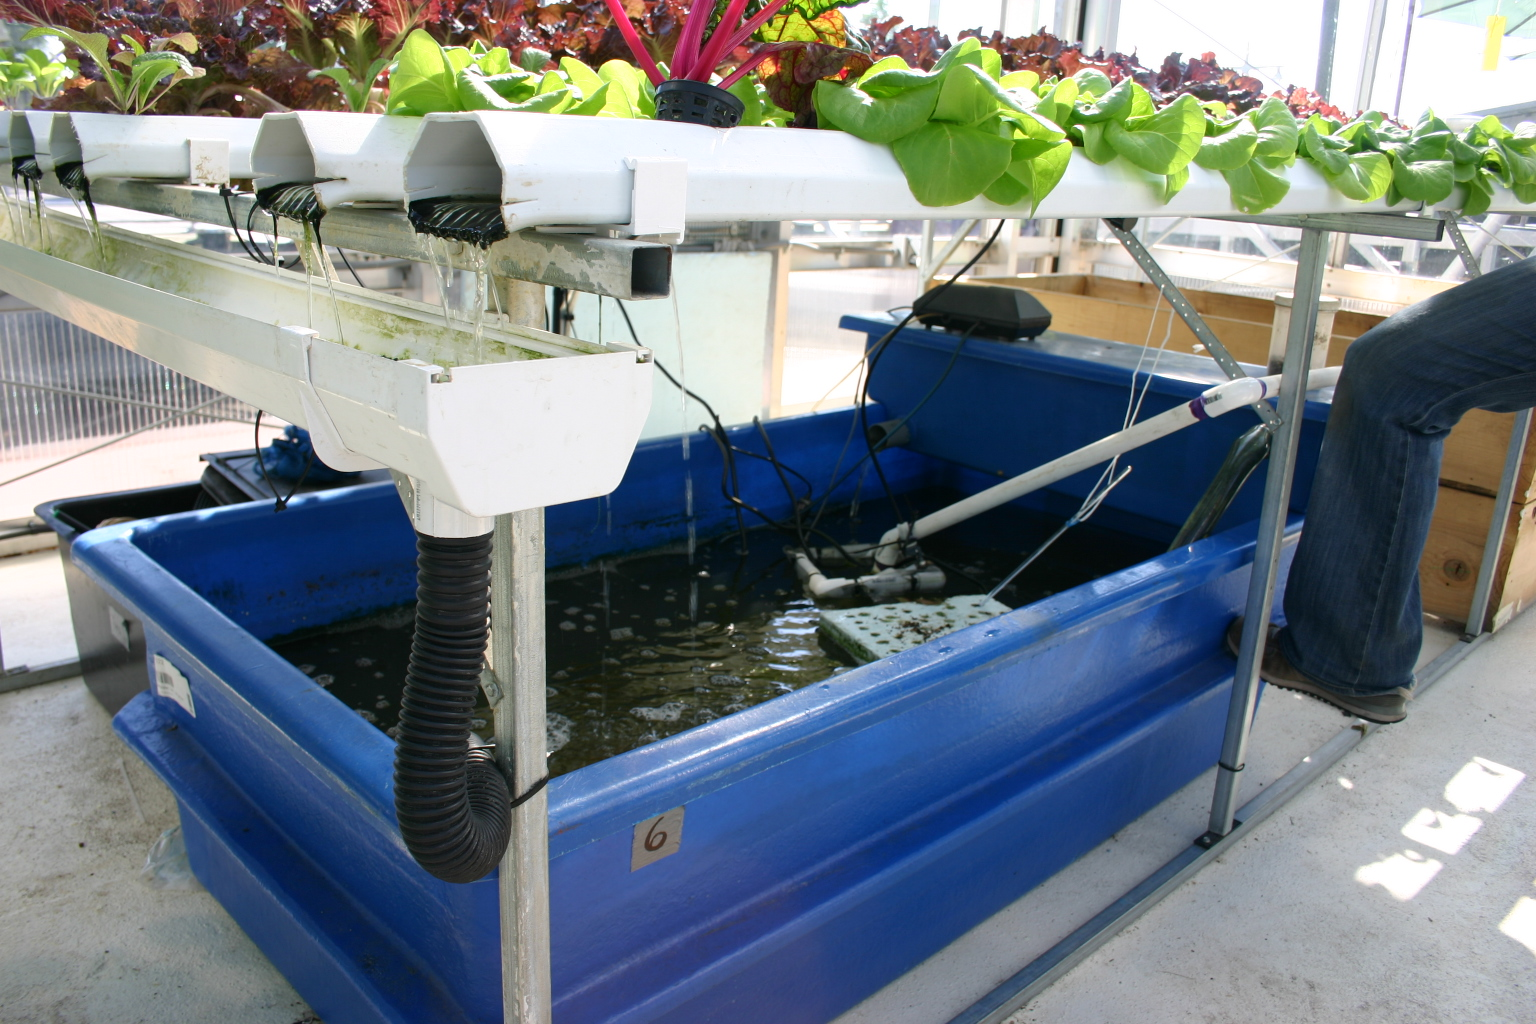
\includegraphics[width=12cm]{image_folder/Aquaponics_with_catfish.jpg}
\Bildquelle{Somma, Ryan; Aquaponics with catfish; 2008;}
\label{fig:aquaponik}
\end{figure}

\subsection{Positive und negative Auswirkungen von UL im Überblick}
     \subsubsection{Mögliche positive ökologische Auswirkungen von UL auf Städte}  


Sofern Landwirtschaft im urbanen Raum und außerhalb (d.h nicht in Fabriken oder abgeschlossenen Räumen) betrieben wird, wirkt sich dies über die Beeinflussung der Temperatur, Luftfeuchtigkeit und CO2-Aufnahme positiv auf das Mikroklima und die Biodiversität der Stadt aus.
Gleicheitig entsteht durch einen vermehrten Pflanzenbewuchs in der Stadt (vor allem bei Bewuchs um Gebäude) eine Milderung des sogenannten Urban -Heat-Effects. Die Gebäude heizen sich im Sommer also weniger auf, was sich wiederum positiv auf die Luftqualität auswirkt und Energiekosten für eventuelle Klimatisierung eingespart werden kann.\footcite{Schulz2013UrbaneLandmanagements},\footcite[Vgl.][S.16]{Spring2012DerBasel-Stadt}

\begin{figure}[htbp]
\centering
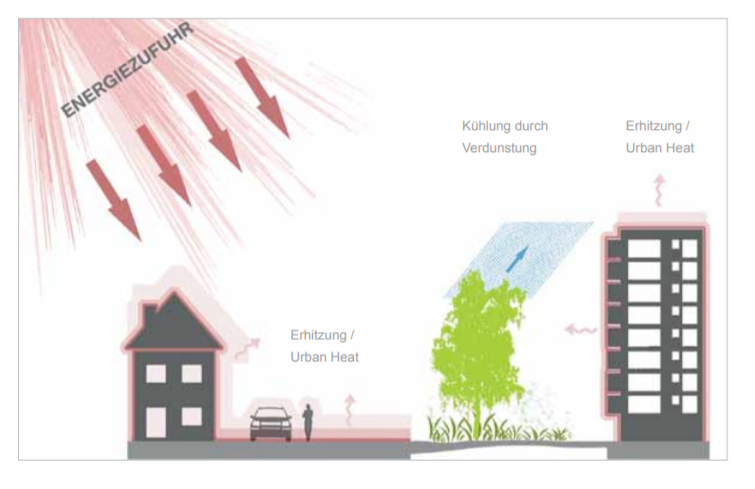
\includegraphics[width=14cm]{image_folder/urbanheat.png}
\caption{Der Urban Heat Effekt}
\label{fig:urbanheateffekt}
\end{figure}
\\

Urbaner Anbau von Lebensmittel und folglich kurze Entfernungen zum Verbraucher, bieten neue Möglichkeiten zur Reduzierung von Transportwegen, Kühlung und Verpackung von Lebensmitteln. Der Bedarf an fossilen Rohstoffen kann auf diese Weise sinken, was sich positiv auf die Bewertung des ökologischen Fußabdrucks der Lebensmitteln auswirkt. Schulz fasst viele wichtige Punkte zusammen: "Kurze, innovative Nahrungsverteilungswege zwischen Erzeugern und Verbrauchern, Transporteinsparungen, frische Produkte, Integration der „Landwirte“ in Marketingprozesse sowie bessere Absprache zwischen Angebot und Nachfrage sind potenzielle Vorzüge gegenüber einer globalisierten Landwirtschaft."\footcite[S.10]{Schulz2013UrbaneLandmanagements} Die starke lokale Nähe zwischen Produktion und Verbrauch lässt ebenso Platz für zukünftige Pläne eines Anbaus je Bedarf. Auf diese Weise könnte unnötiger Lebensmittelabfall verhindert werden. Die Integration in die Stadt ermöglicht auch eine Nutzung der städtischen Ressourcen wie Abwärme oder Abwässer, Es entsteht ein Kreislauf-Effekt der ebenso zur Reduzierung des Bedarfs externen Rohstoffe beiträgt.
Sofern für die Zwecke der urbanen Landwirtschaft innerstädtische Flächen entsiegelt werden, kann eine Verbesserung im urbanen Wassermanagement erreicht werden. Dies kann eine positive Auswirkung auf die Grundwasserneubildung haben und da Kanalsystem kann somit entlastet werden.  
  

\begin{figure}[htbp]
\centering
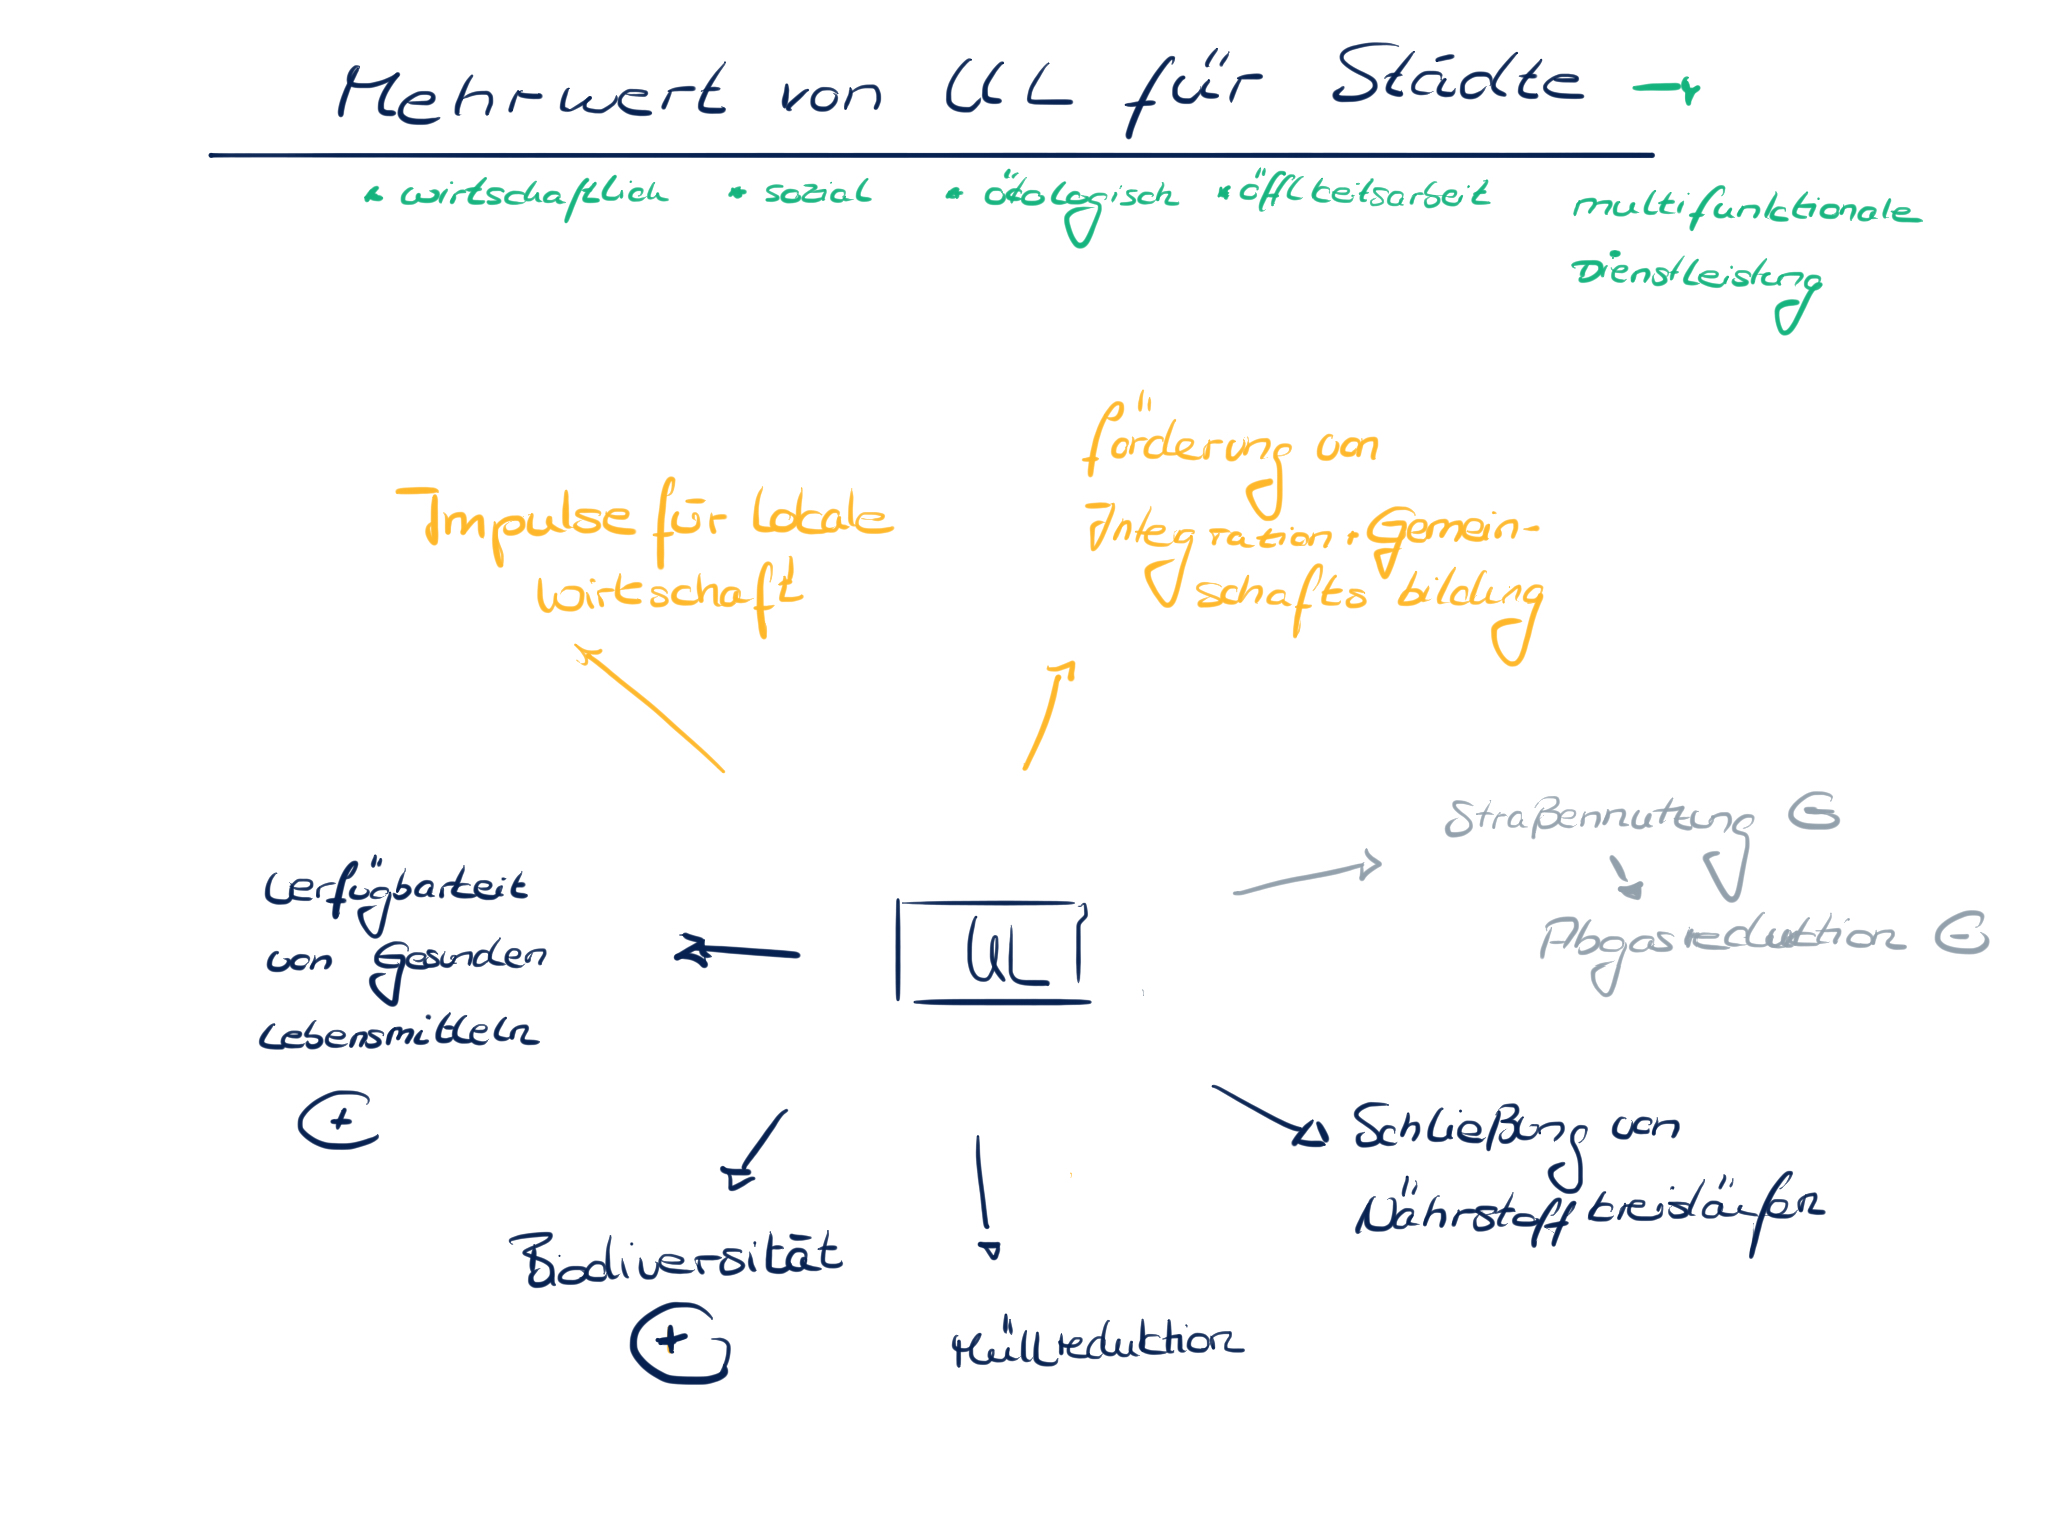
\includegraphics[width=14cm]{image_folder/moeglicheVorteileUL.png}
\caption{Mögliche Vorteile von UL für Städte}
\label{fig:MoeglicheVorteilevonUL}
\end{figure}

\\
Regionalität
\\
Im Vergleich zu konventionellem Anbau sind die Produktionskosten bei VF unabhängig vom Ölpreis (Siehe {Vergangenheit der Urbanen Landwirtschaft} am Beispiel Kuba), was einen deutlichen ökonomischen Vorteil ausmacht.
Ebenso entstehe laut Sharanbir et al durch den Transport \footcite[Vgl.][]{GrewalCanFood}, die Lagerung und Produktion (d.h. Pflügen, Säen, etc.) hoher fossiler Verbrauch.\footcite[]{2012TheEssay}  
laut Despommier werden im Schnitt 30\% der Lebensmittel während Transport und Lagerung durch Druckstellen oder Bakterienbefall/Fäule unverkäuflich.\footcite{Despommier2009TheFarms}
Ein weiterer Vorteil des regionalen Anbaus sei laut Despommier die kurze Distanz zwischen Produktion und Konsumenten. Folglich gelangen die Lebensmittel meist frischer zum Konsumenten, wodurch der Nährstoffgehalt häufig größer ausfalle.\footcite{Despommier2009TheFarms}


     
 \subsubsection{mögliche negative Auswirkungen von UL auf Städte}
 
Da große Arbeitsgeräte wegen enger Umgebung in VF nicht eingesetzt werden können (z.B. aufgrund von geringer Wegebreiten), kann häufig hoher manuelle Arbeitsaufwand entstehen.
     Lautgeringerer Erträge, im Vergleich zu Anbau auf Großflächen (BRINK 2002)
     \item ”erhöhter Arbeits‐ und Koordinationsaufwand aufgrund der Kleinteiligkeit der Verteilung auf verschiedene Stadtbezirke(GALK 2006). "Vielfach ist erst eine Schlaggröße von vier bis fünf Hektar für den Landwirt wirtschaftlich interessant (SENATSVERWALTUNG FÜR STADTENTWICKLUNG 2010)." (Quelle: Urbane Landwirtschaft und Green Production als Teil eines nachhaltigen Landmanagements)
 
\section{Prognose zur urbanen Landwirtschaft}

\subsection{Heutige und zukünftige globale Landnutzung}

Um herauszufinden wie wichtig die Entwicklung von urbaner Landwirtschaft tatsächlich ist, ist es zunächst bedeutend Landwirtschaftsformen auf deren Grundlage zu untersuchen. Die Entwicklung der globalen Landnutzung ist insofern relevant, dass die Landressourcen für eine Versorgung durch Lebensmittel entscheidend sind. Die Versorgung und deren Sicherstellung hängen wiederum stark von der Weltbevölkerung ab. Das Bundesministerium für Umwelt, Naturschutz und nukleare Sicherheit, der Industrieverband Agrar e. V. (IVA) und die Food and Agriculture Organization of the United Nations (FAO) geben an, dass die Weltbevölkerung bis zum Jahr 2050 auf über neun Milliarden Menschen ansteigt.\footcite[Vgl.]{BMU2016GlobaleUmweltfolgen}[sowie]{Agrar0NahrungsmittelLandwirtschaft}[und]{FAO2009How2050} Laut dem Bundesministerium für Umwelt bereite die Lebensmittelproduktion aber bereits jetzt enorme Umweltprobleme. Zudem würden bereits jetzt ca. 800 Millionen Menschen an Hunger leiden.\footcite[Vgl.]{BMU2016GlobaleUmweltfolgen} Der IVA prognostizierte eine pro Kopf Anbaufläche von 1700 Quadratmetern im Jahre 2050. 2010 waren es laut dem IVA noch ca. 2100 Quadratmeter pro Person.{Agrar0NahrungsmittelLandwirtschaft}

Die FAO ging 2009 zudem davon aus, dass fast der gesamte Bevölkerungszuwachs in den Entwicklungsländern stattfinden wird. Die Urbanisierung würde sich fortsetzen und beschleunigen und etwa 70 Prozent der Weltbevölkerung würden städtisch sein. Um diese größere, städtischere und reichere Bevölkerung zu ernähren, müsse die Nahrungsmittelproduktion um 70 Prozent steigen. Die jährliche Getreideerzeugung müsse auf rund 3 Milliarden Tonnen (2,1 Milliarden Tonnen, Stand: 2017 \footcite[Vgl.]{IGC}) steigen, und die jährliche Fleischproduktion müsse um über 200 Millionen Tonnen auf 470 Millionen Tonnen steigen.\footcite[Vgl.][S. 2]{FAO2009How2050}

Die Fleischproduktion betrug laut der FAO 2017 ca. 330.4 Millionen Tonnen. Gleichzeitig prognostiziert die FAO bis Ende 2018 einen Anstieg auf 336.2 Millionen Tonnen.\footcite[Vgl.][S. 7]{} Das statistische Bundesamt veröffentlichte 2010 einen Bericht zur Flächenbelegung von Ernährungsgütern in dem die Flächennutzung für Nutzvieh weltweit auf ca. 13.123.000 Hektar Land geschätzt wird. Das entspricht einer Fläche von ca. 131.230.000.000 Quadratmetern. Der Futterverbraucht lag dabei bei ca. 130.234.000 Tonnen.\footcite[Vgl.][S. 9]{Sttistisches Bundesamt} Die Menge der Fleischproduktion betrug in diesem Jahr ca. 293 Millionen Tonnen.\footcite[Vgl.]{Institute for agricultere & trade Policy}Steigt der Konsom auf über 470 Millionen Tonnen, benötigen wir rein rechnerisch etwa 60 Prozent mehr Fläche zur Aufzucht von Tieren. In einem Zeitraum von 40 Jahren bedeutet dies einen enormen Anstieg des Flächenbedarfs.

Wie viel Fläche verbraucth der "Getreideanbau"?

Wie viel Fläche braucht der Mensch unbedingt?
    Projekt 2000qm

\begin{figure}[htbp]
\centering
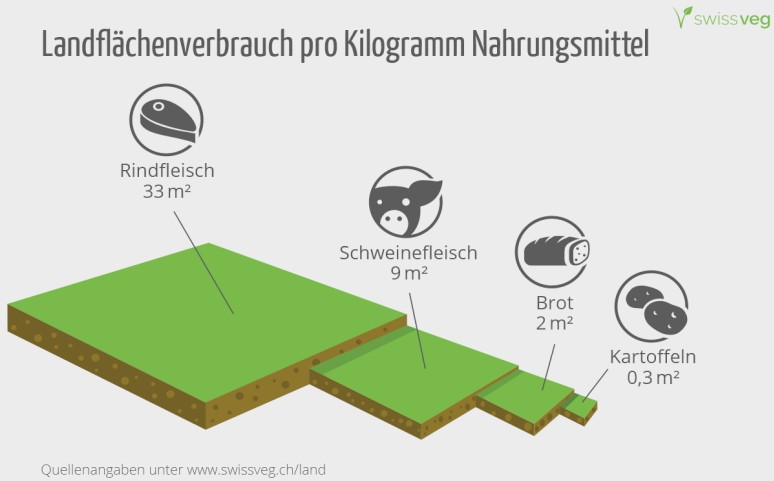
\includegraphics[width=14cm]{image_folder/landverbrauch.jpg}
\caption{Flächenverbrauch pro Nahrungsmittel}
\label{fig:Flächenverbrauch proNahrungsmittel}
\end{figure}<--weiss hier leider nicht ob die quelle seriös ist, vll finden wir was ähnliches

\subsection{Zusammenfassung}

\section{Fazit}

\section{Danksagung}

\newpage
\listoffigures

\begingroup
\singlespacing
\setlength\bibitemsep{10pt} % oder was auch immer
\printbibliography
\endgroup

\end{document}
